\documentclass{ou-report-vaf}

% Dit template is gemaakt door P.J. Molijn in het kader van zijn afstuderen aan de OU in 2014.
% Waarvoor hartelijk dank.
% Minieme maar belangrijke wijzigingen zijn aangebracht door E.M. van Doorn
% Het template is versimpeld door Sylvia Stuurman, 2019.
% Het template is aangepast voor de ba informatica door Harrie Passier, Tanja Vos en Pekka Aho 2020 
% Het tamplate is aangepast met nieuwe huisstyle door Rick Neeft, 2021
% TODO command toegevoegd, 2022

\def\mytitle{How can automated comparison of inferred models help testers finding bugs?}
\def\myauthor{Rick Neeft}
\def\myStudentId{851829973}
\def\myPresentationDate{T.B.D. 2022}

\newcommand{\testar}{\textsc{testar }}
\newcommand{\testarnet}{\textsc{testar .NET }}

\begin{document}

    \pagenumbering{roman}

    % Elements of the thesis
    %%%% TITLE PAGE %%%%%%%
% front cover should be a empty as possible. Title (subtitle) - Name - student Id and thesis presentation date

%to prevent that the title page will be referred as page 1, 
%which will give the warning that there is a page 1 twice.

\pagestyle{plain}

\begin{titlepage}
    \newgeometry{right=100pt,left=58.8pt}

    \pagecolor{ou-light-gray}
    \afterpage{\nopagecolor}
    
    %% Insert the OU logo at the top right corner of the page
    %% PowerPoint contains 84 pt margin in picture
    \begin{tikzpicture}[remember picture,overlay]
                \node at (current page.north east)[anchor=north east,inner sep=58.8pt]{
            
\includegraphics[scale=0.5]{images/ou-text-logo.png}
        };
    \end{tikzpicture}
    
    %% Extra whitespace at the top.
    \vspace*{5\bigskipamount}
    
    %% add title without hypens
    \nohyphens{{\color{ou-red}\Huge\bf \mytitle}}
     
    \bigskip
    %{\large subtitle, if any}
    
    %\bigskip \bigskip
    %by
    \bigskip \bigskip
    
    {\Large\bf \myauthor}\\
    {\large\myStudentId}
    
    {\myPresentationDate}
    
\end{titlepage}

% reset geometry since we changed them for the title page
\newgeometry{right=0.875in,left=.875in}

%%%% END TITLE PAGE %%%%%%%

    % Page 2 must be left blank
    \myemptypage
    
    % Page 3 contains all compulsory data.
    \addcontentsline{toc}{chapter}{Compulsory data}

\myauthor, \myStudentId\\
\textbf{\mytitle}\\
\myPresentationDate
\vspace*{\fill}

Open University of the Netherlands, Faculty of Science\\
Master's Programme in Software Engineering\\
\\
Graduation committee

Chair: Prof. Dr. Tanja E.J. Vos\\
Primary supervisor: Dr. Pekka Aho\\
Seconday supervisor: Fernando Pastor Ricós

Course code: IM9906
\newpage
    
    % Acknowledgements
    %\chapter*{Acknowledgements}
\addcontentsline{toc}{chapter}{Acknowledgements}

I want to thank my supervisors, Pekka Aho, Fernando Pastor Ricós and Tanja Vos, for the opportunity and support of my graduation project. The weekly meeting and feedback were always inspiring and gave me good directions on what to do. I am grateful for allowing me to develop the application in C\#. Besides academic learning, using C\# and Blazor is extremely helpful in my day-to-day career.

Thanks to WithSecure, especially Joona Oikarinen and Tatu Aalto, for their input and feedback regarding the Analysis website and the docker setup.

I want to thank my wife for her support and for allowing me to sit in our home office for countless hours. 

Thank you to my family, and special thanks to my mother, who always supported me and pushed me to achieve my life goals. 

Last but not least, I want to thank my employer, VECOZO, for providing me with time and resources to finish my Masters. 

Rick Neeft\\
\myPresentationDate
    %\myemptypage
    
    % Table of contents
    \begingroup
        \hypersetup{linkcolor=black}
        \tableofcontents
    \endgroup
    \newpage
    
    % Summary
    %\chapter*{Summary}
\addcontentsline{toc}{chapter}{Summary}
lorem ipsum blah blah yadda yadda yadda
    %\newpage
    
    % the content of the thesis
    \pagenumbering{arabic}
    
    \chapter{Introduction} \label{introduction}
    
Regression testing is considered a good practice when testing new software versions before being released to the general public. 
However, due to shortened release cycles, the time to market has decreased drastically. As a result, software test teams have less time to test all new software features, let alone try all other elements to prevent unwanted side effects \cite{rapid-release-cycle-issues}.
The research proposed aims to apply change detection between two versions of the GUI of the system under test. 

This section introduces the proposed research discussing the background and context, followed by the research problem, research aims, research questions and why this research is important.

\section{Background}
The TESTAR tool solves a significant obstacle when it comes to testing the GUI. With TESTAR, the tester can automatically start testing the GUI without any upfront scripts. TESTAR automatically generates and executes test sequences based on elements derived from the GUI \cite{VosAho2021}. In recent master graduation assignments, TESTAR has been extended with an inferred model generation module \cite{thesisMulders}, and it became easier to integrate TESTAR in build and release pipelines in a DevOps environment \cite{thesisSlomp}. Those two additions make it easier to run TESTAR upon each source code integration and retrieving an inferred model about the GUI. In a proof of concept, two inferred models are compared to get changes between versions of the SUT \cite{stateDiff}.

Some companies might write down changes of the software in a changelog. However, some changelogs might not be complete and unwanted side effects might be missing entirely. Comparing two inferred models shows all the changes between versions of a SUT, even the unwanted ones.

\section{Research problem}
Although the proof of concept for change detection is a good start, it lacks some basic functionality. For example, it compares calculated abstract hashes with each other. As a result, even the slightest change in GUI results in a removed and added state between versions.

In addition to change detection, the change visualisation does not use the build-in visualisation tool. The proof of concept generates an HTML-based report, making it difficult to see where the change can be found and which steps the tester needs to take to navigate to the changed state in the software.

\section{The aim of the research}
The research aims to apply change detection on the inferred model created with the automated GUI testing tool TESTAR and research whether the outcome is helping testers finding bugs quicker. The main research questions are:

\begin{questions}
    \item How to detect changes between two versions of the SUT?
	\item How to visualise the detected differences to the user? 
\item How to validate the results of \ref{rq:detect-changes} and \ref{rq:diff-visualisation}?
\end{questions}

\section{Scope}
The scope of the research is change detection in GUI inferred models created by TESTAR. Researching how to make models and making significant changes to the creation of models are omitted. However, tweaking the model generation, like adding data that is not saved at the moment, and configuring TESTAR to create a good model, are in scope.

\section{Contribution}
When change detection is available in TESTAR, it becomes easy for testers to run the comparison in a continuous integration environment and receive an overview of the changes found in an updated version of the software.

As a side effect, the comparison and visualisation solutions can run outside the context of TESTAR and can be deployed to a docker environment.

\section{Document outline}
This research proposal is structured as follows. In section \ref{intoduction} the context, aim and objectives for this research proposal are introduced, together with the limitations for the expected outcome. Section \ref{background} describes the background of this proposal and contains knowledge that is available but might not be known by the readers. Section \ref{releatedWork} includes an overview of the material that can be seen as a direct foundation for this proposal or work that influences the expected outcome. Section \ref{questions} formulates the research questions for the thesis. The last section \ref{planning} will outline the chosen approach and planning for the graduation assignment.
    \newpage
    
    \chapter{Background} \label{background}

\todo{make better introduction for the chapter. }

This section describes the background of this proposal and contains information that is available but might not be known by students and readers. 

\section{Introduction into GUI Testing}
Ever since the first line of software is written, testers are testing its workings. While in the early day of software, the \acrfull{ui} was mainly terminals based or a set of blinking LEDs \cite{altair8800} \footnote{For example the ALTAIR 8800 computer \cite{altair8800}}, today we have an ever-increasing amount of \acrfull{gui} applications. Testings a GUI application is labour intensive and costs a lot of money \cite{gui-history}.

Initially, testers were using \acrfull{cr} software to automate their work. A tester would record a test scenario into the CR software, and then the CR software will execute the test case when needed. Using CR software, the time required to retest software decreases; however, the big downside is that when software changes, so must the recorded scripts \cite{gui-history}.

Then came \acrfull{mbgt}. With MBGT, the GUI elements and behaviour are abstracted on a higher level. The created models are used to generate abstract test cases. Those abstract test cases need to be mapped or transformed to get concrete test cases that are executed on the SUT. The downside of MBGT is the effort required to create the models and the need to have formal modelling expertise. Formal modelling expertise is not needed with the latest evolution in test automation: model inference. 

The \emph{model inference}, also known as model extraction and GUI Ripping \cite{gui-ripping}, is the current state-of-the-art approach to automate GUI testing \cite{gui-history}. Inferred models are state graphs based on the GUI of the SUT. There are two ways to generate inferred models; the first is a static approach where the source code of the  SUT is used to create a GUI model. The second is a dynamic approach where the GUI state is captured and extracted while being executed. 

The static approach has several downsides. First, the source code must be available, which is not always the case and secondly, it is challenging to capture behaviour based on the GUI source code. For example, with HTML, it is easy to generate a model; however, its behaviour is either in Javascript or server code.  It is possible to overcome those stumbling blocks by executing the SUT.
    
As for the Dynamic approach, it captures the model during test execution. The automated test tool interacts with the SUT in a scriptless and random way. This random scriptless approach is called \emph{Monkey testing}. Usually, test monkeys have no idea in which state the SUT is in and what type of input is allowed. It is therefore essential to make the test monkey smarter. A "smart test monkey" can be achieved by making them "see" the UI elements (Section \ref{data-retrieval}). Section \ref{testar-testauto} will give more details about how \testar is using smart test monkeys.

\section{What is \testar?} \label{what-is-testar}
\testar - or TEST* - is an automated software testing tool for the GUI level \cite{testar-about}. \testar started within the context of the \acrfull{fittest} project. \testar is open-source, the source code is published on GitHub \footnote{ \url{https://github.com/testartool/testar\_dev}}. A screenshot of the \testar tool is displayed in Figure \ref{fig:testar}.

\bigskip
\begingroup
\captionsetup{type=figure}
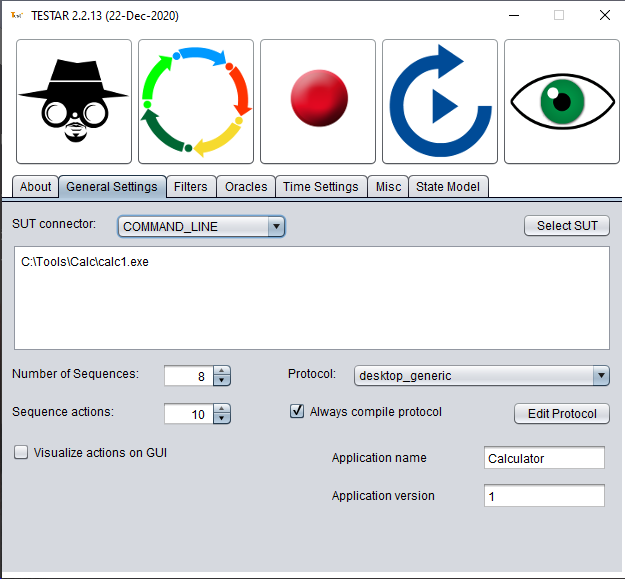
\includegraphics[scale=0.5]{images/testar.png}
\captionof{figure}{Screenshot of the \testar tool}\label{fig:testar}
\endgroup

\testar has several \emph{execution modes} in which it interacts with the SUT \cite{testar-manual}. From left to right, in figure \ref{fig:testar}, those are Spy, Generate, Record, Replay and View mode.

The \emph{Spy} mode allows the user to inspect a SUT and analyse how \testar is interpreting the widgets on the screen. Figure \ref{fig:calc-spy} shows the Windows calculator in spy mode. Dots on the GUI indicate actions that \testar could execute to interact with the SUT. Furthermore, within \testar, it is possible to filter out actions. Then, \testar will not execute those actions. The filtered actions are marked with a grey-coloured dot. A list with properties about the widget is shown when hovering, as well as a unique identifier of the current \emph{state}, more information about the state and the unique identifier can be found at section \ref{gui-state}.\par

\bigskip
\begingroup
\captionsetup{type=figure}
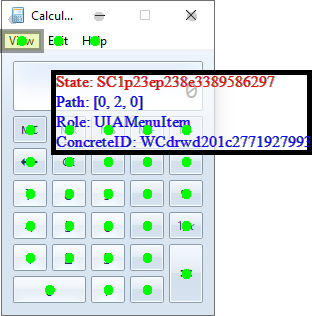
\includegraphics{images/calc-state.png}
\captionof{figure}{Screenshot of the Calculator with \testar Spy}\label{fig:calc-spy}
\endgroup

In the \emph{Generate} mode, \testar will start testing the specified system. Section \ref{testar-testauto} gives more details about \testar test automation.

The \emph{Record} mode allows a tester to record a test sequence manually. In the \emph{Replay} mode, existing test execution can be re-executed and lastly, the \emph{View} mode allows existing test executions to be viewed.

\newpage
\section{TEST automation} \label{testar-testauto}
\testar works without test scripts. Instead, it uses GUI Ripping and Monkey testing techniques. \emph{GUI Ripping}, first introduced by Memon et al. \cite{gui-ripping}, is a process to obtain the GUI's structure and execution behaviour automatically. As for \emph{Monkey testing}, it is a process in which decisions (interactions with the GUI) are randomly made. Section \ref{data-retrieval} will give more insights into GUI Ripping.

\testar is using a flow to execute tests on the SUT. This flow is as follows:
\begin{samepage}
\begin{enumerate}
    \item Start the SUT
    \item Scan the GUI and obtain the state (Section \ref{gui-state})
    \item Finding and selecting an action to execute
    \item Evaluate state with a test oracle (Section \ref{test-oracles})
    \item Stop the SUT when no actions are left to be executed or restart the SUT when more sequences are required.
\end{enumerate}
\end{samepage}

\bigskip
\begingroup
\captionsetup{type=figure}
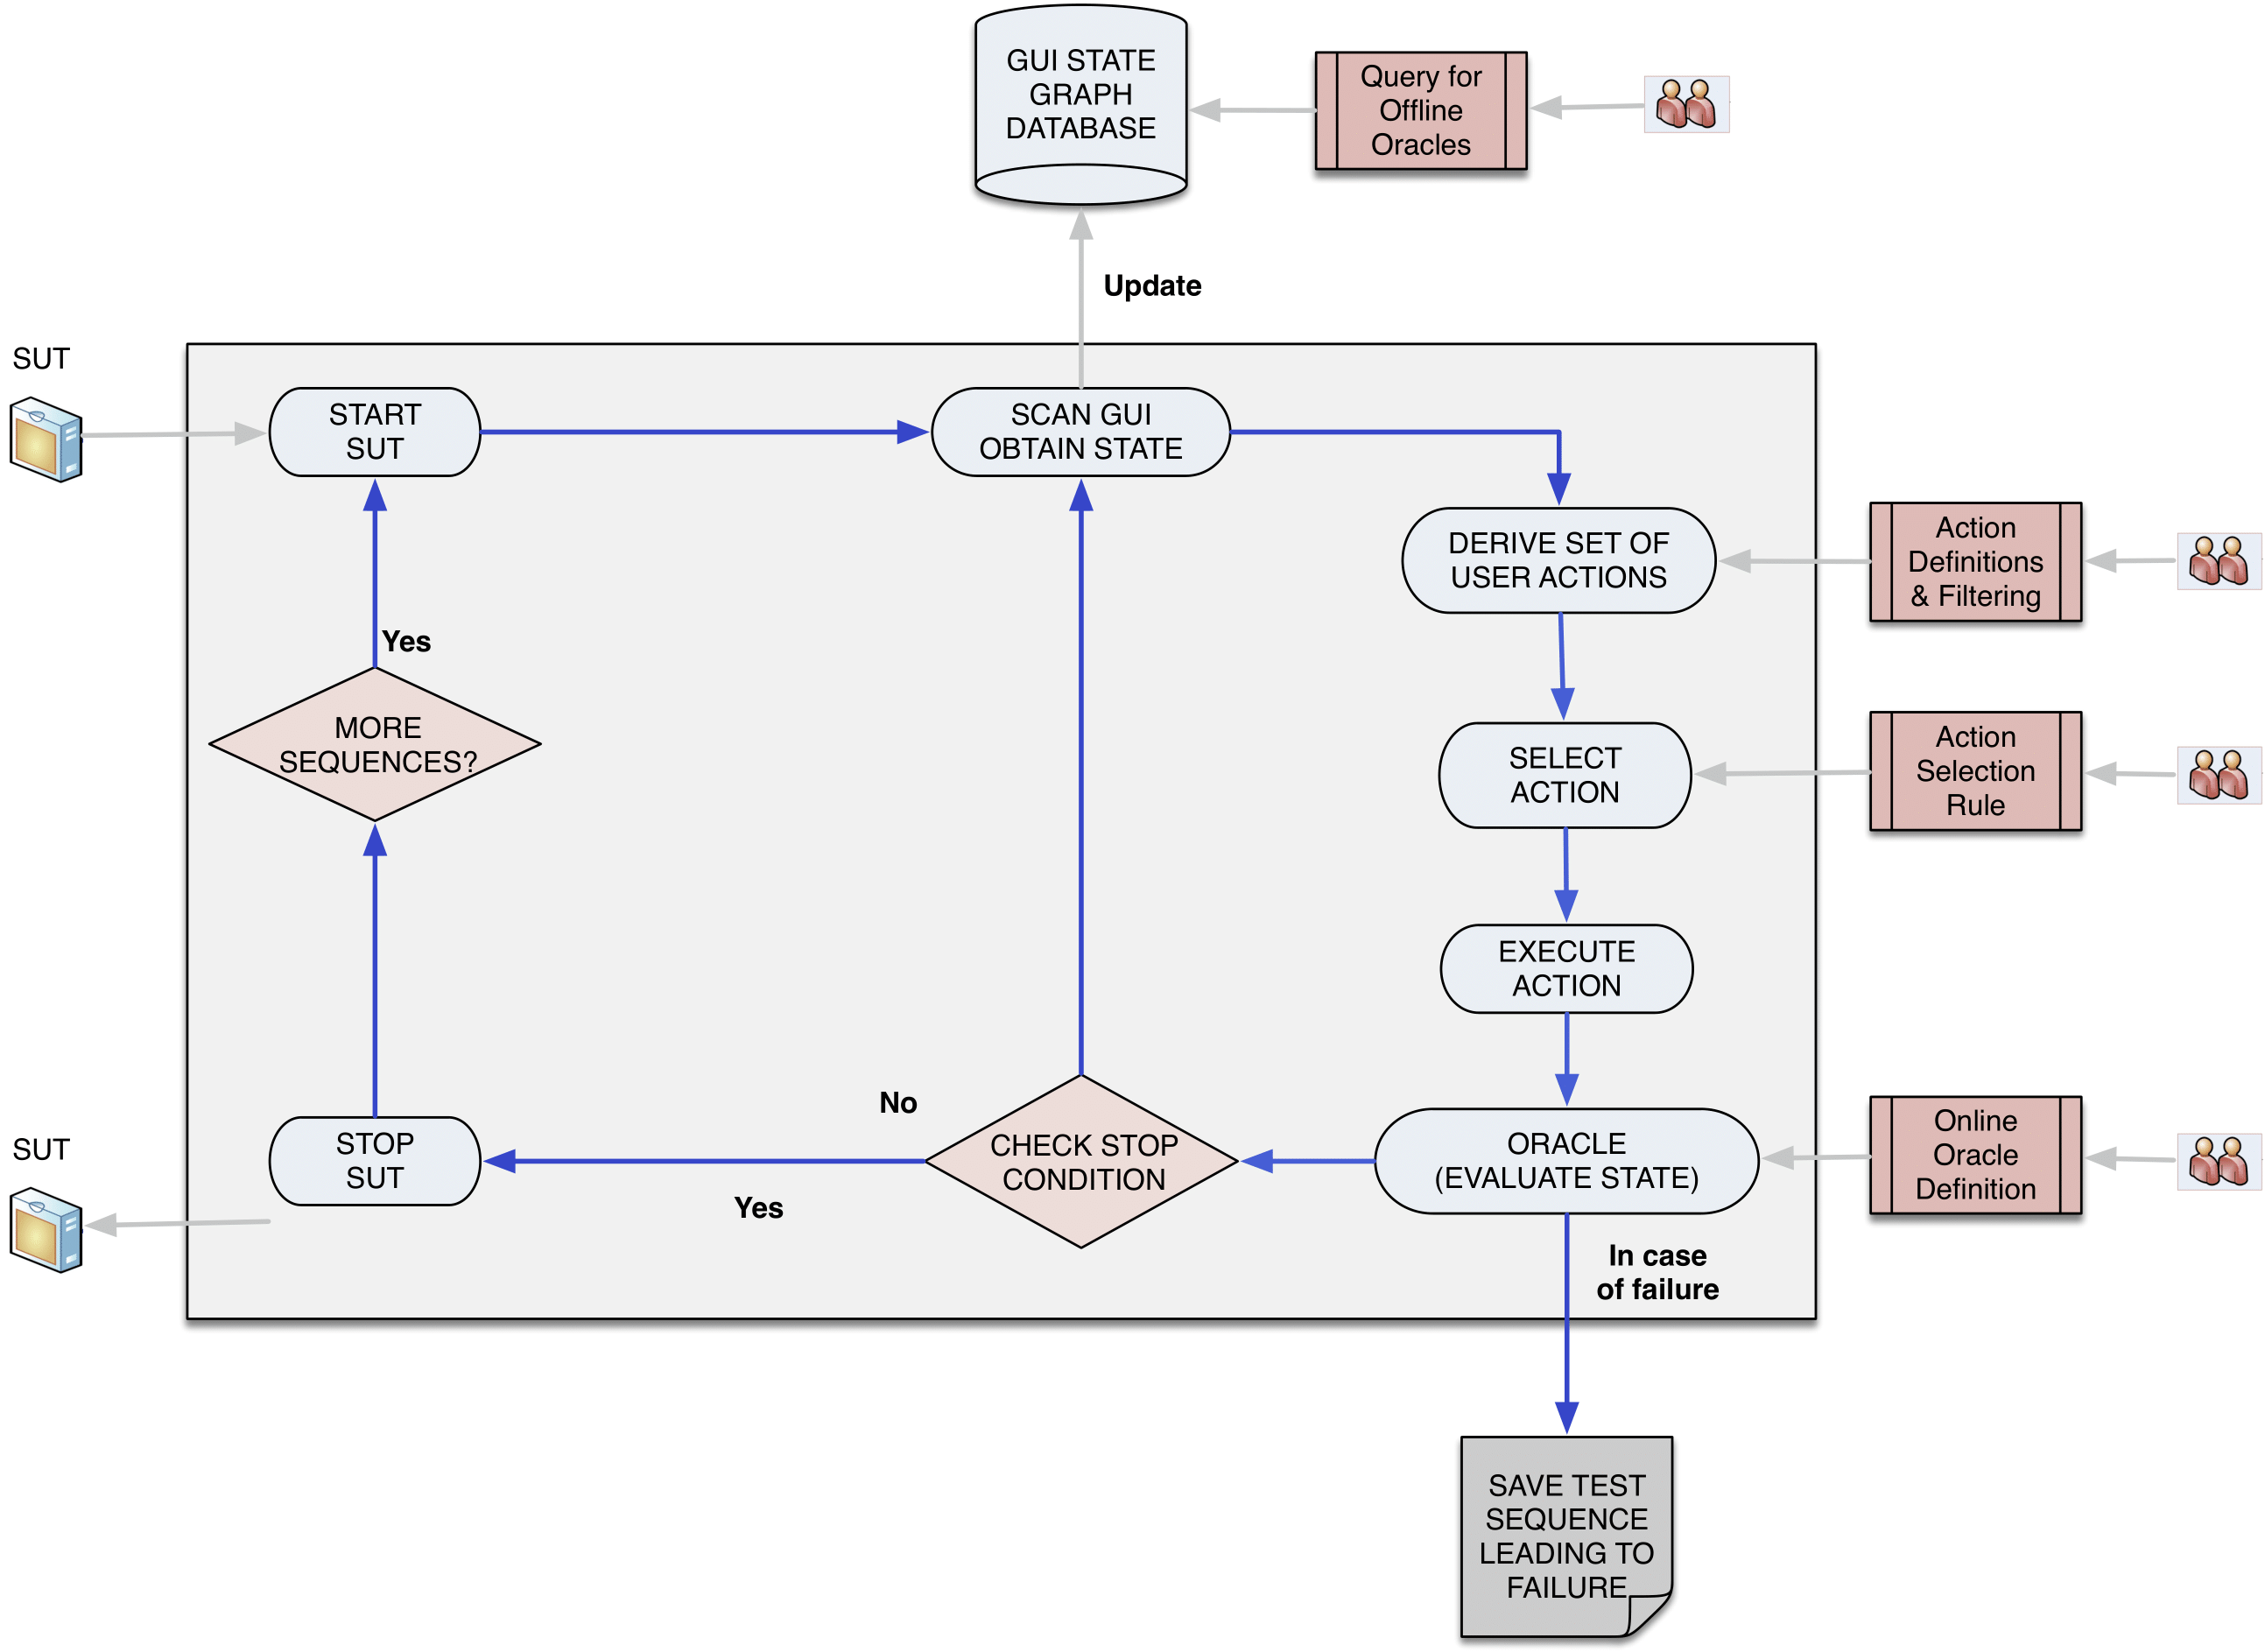
\includegraphics[scale=0.36]{images/testar-test-cycle.png}
\captionof{figure}{\testar test cycle \cite{VosAho2021}}\label{fig:testar-test-cycle}
\endgroup

Figure \ref{fig:testar-test-cycle} shows the flow graphically \cite{VosAho2021}. The test specialist needs to provide SUT details to \testar, like which actions should not be executed, and devise a mechanism that defines which SUT behaviour is correct and which is not, named a test oracle (Section \ref{test-oracles}). 

\section{How is the SUT tested} \label{test-oracles}
When software is tested, a method is needed to check the correct behaviour of the SUT. The method of checking is formally known as a \emph{test oracle} \cite{testOracles}. 

Outside the \testar context, an example of a test oracle could be an \emph{assertion} in software code. An assertion is a boolean expression created in a program by a software developer which checks the program's behaviour during run-time \cite{barr2014oracle}. Assertions can also be used in unit tests as displayed below on Listing \ref{code:assert}. 

\begin{lstlisting}[language=Java, caption=Example assertion, label=code:assert]
@Test
public void testAdd(){
    Calculator sut = new Calculator();

    int expected = 3;
    int actual = sut.Add(1,2);

    Assert.assertEquals(expected, actual);
}
\end{lstlisting}

\testar comes with some test oracles out-of-the-box. Without any configuration, \testar will recognize crashes and unresponsiveness. It is also able to validate the GUI state with suspicious text. For example, a test sequence will fail when the title of a widget contains the word 'exception'. The input for the suspicious text is a regular expression that can be adjusted by the \testar user \cite{VosAho2021}. 

\subsection{Online and Offline Test oracles}
Test oracles come in two variants, \emph{online} or \emph{on-the-fly} test oracles and \emph{offline} test oracles \cite{VosAho2021}. With online test oracles, the state under test is being asserted for any anomalies during test execution. For example,  an online test oracle inspects the URL to check for any information being exposed in the query string. Offline test oracles will look into stored data - like logs - to find anomalies after test execution. For example, offline test oracles can inspect all the visited URLs to check for any exposed information in the query strings.

The two test oracle variants are complementary to each other and can run side by side. However, each variant comes with its strengths and weaknesses. The online test oracle takes up computation time because it inspects the state during test execution. This inspection of state slows down the test execution and may become an issue with time-critical SUTs. On the other hand, some issues - like the SUT becoming unresponsive - can only be checked during test execution. An offline test oracle is inspecting the gathered data after test execution has finished. Especially with larger data sets, this can become helpful. Inspecting the data may run in parallel, which can speed up the test oracle. Additionally, when developers create new offline test oracles, they can inspect the recorded data instead of executing a new test run \cite{de2019offline}.

\section{How is data retrieved} \label{data-retrieval}

Section \ref{testar-testauto} discussed how \testar is using GUI ripping to obtain the GUI's structure. A GUI consists of a non-empty set of UI components, known as \emph{widgets}. Examples of widgets are Windows or buttons; more examples can be found in Table \ref{tables:widgets} \cite{VosAho2021}. 

\begingroup
\captionsetup{type=table}
\begin{tabularx}{\textwidth}{ 
  | >{\raggedright\arraybackslash}X 
  | >{\raggedright\arraybackslash}X 
  | >{\raggedright\arraybackslash}X | }
    \hline
    Windows & Menus & Controls \\
    \hline
    \hline
    main windows & menu bars & buttons \\
    child windows & dropdown menus & textboxes \\
    popup windows & context-aware menus & links \\
    && radio buttons \\
    && checkboxes\\
    && dropdown select boxes\\
    && sliders\\
    && tabs\\
    && scrollbars \\
    \hline
\end{tabularx}
\captionof{table}{Example of GUI widgets \cite{VosAho2021}}\label{tables:widgets}
\endgroup

The widgets are structured hierarchically in a \emph{widget tree}. Each node in the tree is a widget with its related properties, such as the title, position and role. In figure \ref{fig:widget-tree} a compact widget tree is shown for the calculator. 

\bigskip
\begingroup
\captionsetup{type=figure}
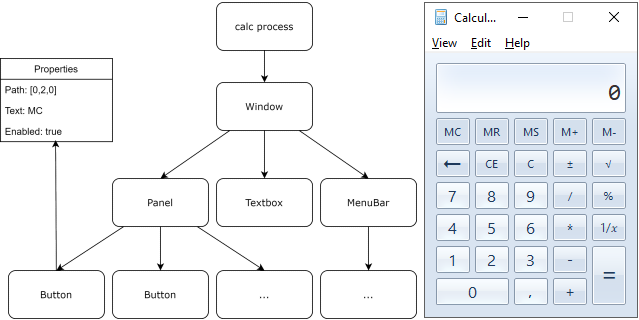
\includegraphics[scale=0.7]{images/calc-tree.png}
\captionof{figure}{A compact version of a widget tree for the calculator.}\label{fig:widget-tree}
\endgroup

\section{Widget data API}

In order to retrieve data from a SUT, \testar is making use of external APIs to access widgets that are part of the GUI \cite{thesisMulders}. \testar is using three different APIs.

In order to test a desktop application, \testar makes use of the Windows Automation API. The purpose of the Windows Automation API is to expose rich information about UI elements\cite{win-api-info}. For web applications, \testar uses Selenium Chromedriver. The Chromedriver is a tool for automated testing. It provides capabilities for navigating through web pages, user input, and JavaScript execution \cite{chrome-driver-info}. The latest API that \testar is using is Appium. Appium is a test automation tool for native, mobile web, and hybrid applications on iOS mobile, Android mobile, and Windows platforms \cite{appium-info}.

\section{GUI State} \label{gui-state}
In the previous sections, the widget tree is discussed and how the widgets are retrieved. In the widget tree, all the GUI elements with their properties are captured. The widget tree represents the state of the GUI when it has stopped executing any action. The GUI is at 'rest'. When an action is executed, the GUI can change, going to a new state. In figure \ref{fig:state-actions} the state change is represented in a small graph. 
\bigskip
\begingroup
\captionsetup{type=figure}
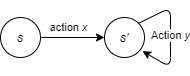
\includegraphics{images/state-action.png}
\captionof{figure}{An graph with two states and two actions.}\label{fig:state-actions}
\endgroup

The graph is a directed graph since every action changes the GUI from one state to the other. An action may lead to the same state, see figure \ref{fig:state-actions} action \textit{y}. However, that would mean that the action does not do anything or \testar does not indicate a change. For example, the GUI changes but the property corresponding to the change is not included in the widget tree.

The universe of states and actions of the SUT's GUI makes up an inferred model. More information about the inferred model and how they are created can be found in section \ref{inferred-model}.

\section{How is data persisted}

\testar is using a database to store and retrieve state model data. Gier and Kager investigated which data storing solution would be beneficial to \testar \cite{GierKager}. The data solution must comply with six requirements. Generally speaking, the requirements were as follows: an open-source graph database with a straightforward query mechanism. The conclusion was that OrientDB was the best solution that met all the requirements.

\begin{samepage}
OrientDB is a Multi-Model NoSQL \acrfull{dbms} that combines four models \cite{orientDbModeling}:

\begin{itemize}
    \item \hyperlink{db:key-value}{Key/Value}
    \item \hyperlink{db:document}{Document}
    \item \hyperlink{db:graph}{Graph}
    \item \hyperlink{db:object}{Object}
\end{itemize}
\end{samepage}

A \hypertarget{db:key-value}{\emph{Key/Value}} is the simplest model and allows storing information (value) that is accessible with a key. Key/Values can be grouped into \textit{buckets}. However, OrientDB supports richer models in the form of document and graph elements.

A \hypertarget{db:document}{\emph{document}} is a schema-less set of key/value pairs. The \emph{key} allows access to the corresponding value. OrientDB allows the developer to store documents into \emph{clusters}. Relations between document are either embedded into other document or \emph{linked} to each other. Someone familiar with relational databases can view a cluster as tables, a document as the row and the key/value pairs are columns.

The \hypertarget{db:graph}{\emph{graph}} is a model consisting of \emph{Vertices} and \emph{Edges}. Vertices are the nodes in the graph, and the edge is the link between those nodes. In \testar terminology, a vertex represents state, and the edge is an 'action' from one state to the next. A Vertex consists of three elements: a unique identifier, a set with incoming Edges and outgoing Edges. An edge consists of four elements: a unique identifier, an incoming vertex (\emph{head}), an outgoing vertex (\emph{tail}) and a label that describes the relationship between the head and tail vertex.\par

The last model is the \hypertarget{db:object}{\emph{object}} that supports inheritance, like in the Object-Oriented programming paradigm.\par

Despite being a NoSQL database, OrientDB does support SQL as a query language \cite{sql-lang} albeit that it does not support all SQL statements. The majority of developers have experience with SQL \cite{sql-stats}, and as a result, new developers and students can start querying the \testar data and start expanding its features.\par

In addition to \testar, other applications can query the state model data in the OrientDB database as well. For example, developers and students can create external tools for a single purpose, like a state model difference application. When building external tools, the \testar application can be kept small and focus upon one objective: testing GUI applications. 

\section{The Murphy tools} \label{murphy-tools}

\todo{This section should go to chapter 3, leaving it here until comment is resolved}

F-Secure, a security software company, based in Finland, developed the Murphy tool \cite{aho2013industrial}. With the Murphy tool, it was possible to automatically extract models from the GUI and use them for GUI testing. The goal of the Murphy tool is to find as many states of a GUI as possible. Users can customise the Murphy scripts to direct the tool to particular cases. 

Like \testar, Murphy creates a directed graph of the GUI under test. Each vertex of the graph is a state of the GUI represented by a screenshot of the GUI. Each edge is an action that the user could perform. 

Like \testar, Murphy is a platform-independent test tool. To accomplish that, Murphy uses various drivers. A driver recognises elements and windows of the GUI under test. One of the drivers uses the 'tab' key to enumerate UI elements. 

While Murphy is crawling the GUI it is making screenshots of the GUI. Besides that, the screenshots represent the state in the graph; they are used to detect changes between different versions of the SUT. 

\section{Inferred model} \label{inferred-model}
The master thesis by Mulders had two significant outcomes. The first is an inferred model module, and the second is the visualisation of the inferred models \cite{thesisMulders}. The visualisation module is a web-based application that shows the inferred model with screenshots and properties. Although the visualisation module will be required when we want to visualise the results of the change-detection software, it is not necessary to go into depth in this document. This section will discuss what an inferred model is and how they are generated. 

The GUI state was discussed in section \ref{gui-state}. The section ended with the sentence that the universe of states and actions of the SUT's GUI makes up the inferred model. The inferred model is a directed graph showing the GUI-state of the application and the transactions between states. The vertex of the graph represents the GUI-state. Each vertex has a set of incoming and outgoing edges, called the actions. 

Figure \ref{fig:state-model} shows the result of the inferred model in the visualisation module.

\bigskip
\begingroup
\captionsetup{type=figure}
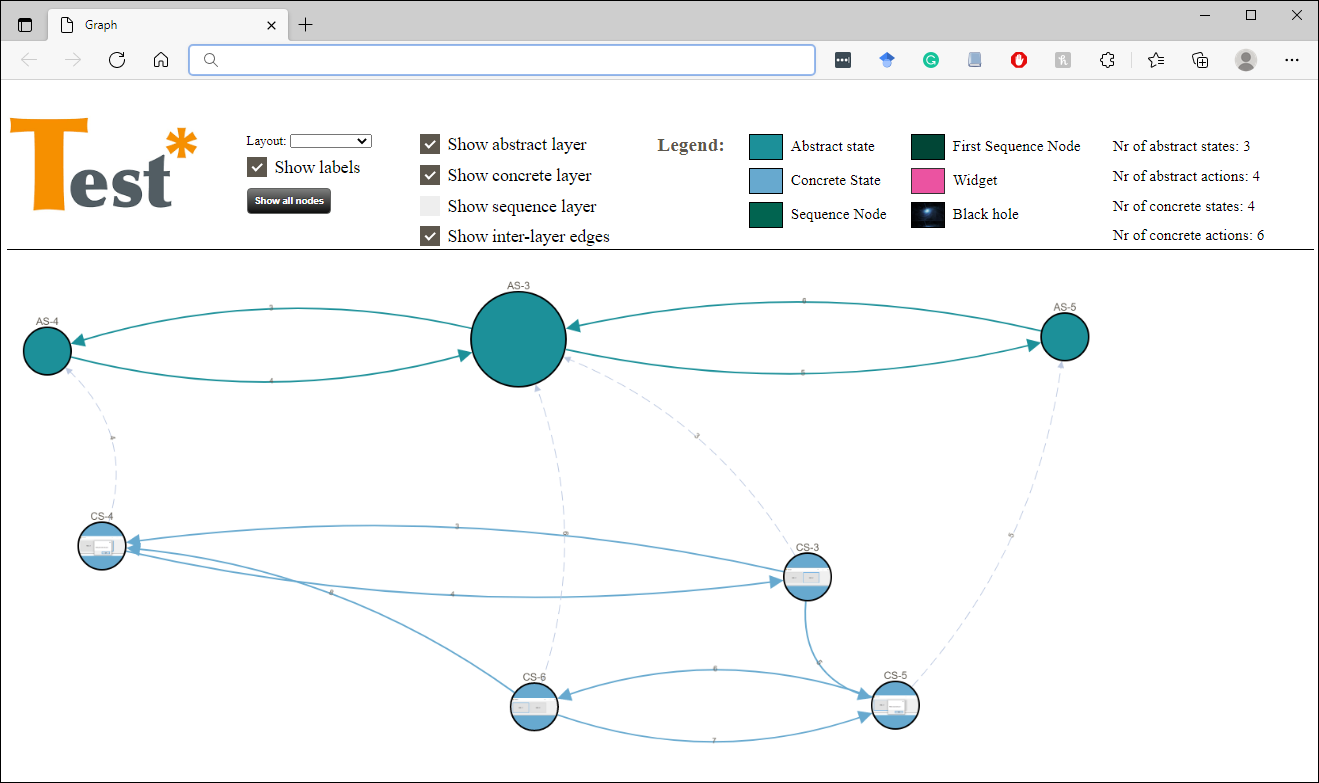
\includegraphics[scale=0.38]{images/state-model.png}
\captionof{figure}{an inferred model in the visualisation application}\label{fig:state-model}
\endgroup

In figure \ref{fig:state-model} two models can be observed. The first model, indicated by the AS text, shows the abstract model. The second, indicated by the CS text, shows the concrete GUI states. 

\subsection{Concrete model}
The concrete model contains all the data that could be retrieved from the GUI. The identification key uses a hash calculated over all the properties. Aside from the widget's properties, the concrete models also contain a screenshot of the GUI for each state \cite{thesisMulders}.

Figure \ref{fig:concrete-node} shows an example of a node in the concrete model. Upon selecting a node, the properties of the node show, including the screenshot taken during the test. The grey dotted line, indicated with the letter 'a', shows the connection with the abstract node, see section \ref{abstract-model} and figure \ref{fig:abstract-model} for more details. The two outgoing edges, indicated with the letter 'b', shows the two actions available in this state. The incoming edge, indicated with the letter 'c', shows how the state was reached. 

\bigskip
\begingroup
\captionsetup{type=figure}
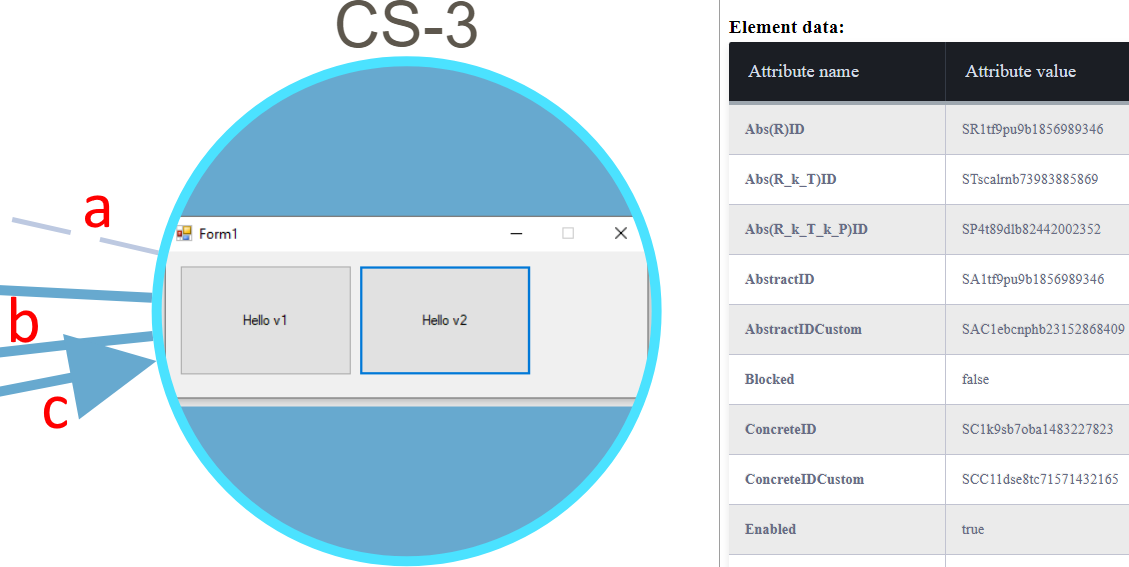
\includegraphics[scale=0.5]{images/concrete-model.png}
\captionof{figure}{A node from the concrete model}\label{fig:concrete-node}
\endgroup

\newpage
\subsection{Abstract model} \label{abstract-model}
Since the concrete models contain all the data from a GUI-state, they can become quite large.  Therefore an abstract state model is made \cite{thesisMulders}. Figure \ref{fig:abstract-model} shows an example of such a abstract node. The grey lines (from CS-3, CS-6 to AS-3) indicates which concrete states are abstracted. The properties of the abstract node are displayed, what the identifier is and which concrete state(s) it represents.

\bigskip
\begingroup
\captionsetup{type=figure}
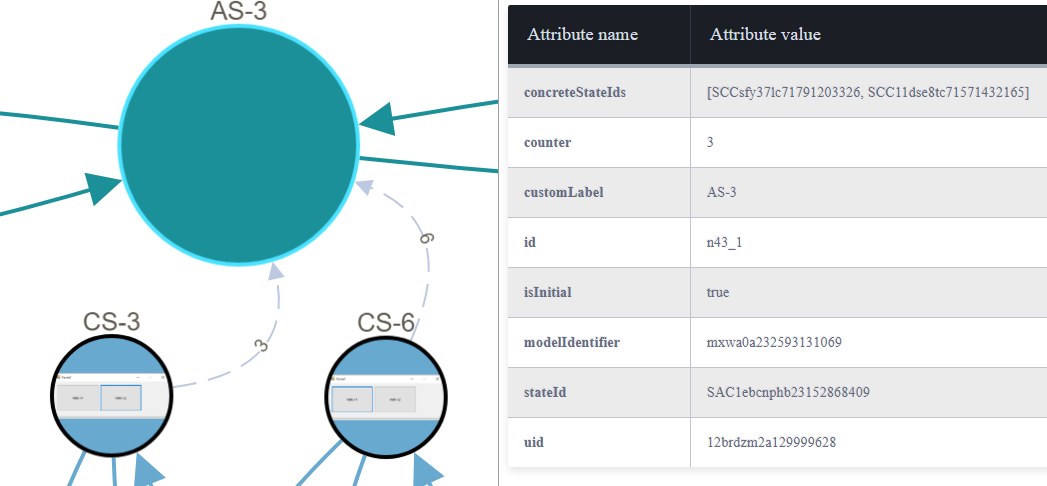
\includegraphics[scale=0.5]{images/abstract-model.png}
\captionof{figure}{A node from the abstract model}\label{fig:abstract-model}
\endgroup

\subsection{State identifiers} \label{state-identifiers}
Every state must have a unique id for identification. The identifier is calculated with the data from the widget tree. 

\testar uses a hashing algorithm that works as follows: the widgets' properties are concatenated and hashed. The outcome will be used as the identifier for a widget. The hashes from the widget in the widget tree are then combined and hashed to create an identifier for the GUI state \cite{VosAho2021}. The \testar's algorithm is similar to how a Merkle tree works, more information can be found at section \ref{merkle-tree}.

To identify the state (and actions), \testar calculates two state identifiers; an abstract and concrete state identifier. For the concrete state identifier, all the properties of a widget are used. For the abstract identifier, a subset of the properties is used. It is configurable which properties are used for the abstract identifier. By default the properties \textit{role}, \textit{title}, \textit{position} and \textit{enabled} are utilised \cite{VosAho2021, thesisMulders}.

When running \testar, it is possible to configure which widget properties should be used for the abstract state identifier. Figure \ref{fig:advance} shows the selection dialogue in which the user can select the properties for the abstract identifier.

\section{Merkle tree} \label{merkle-tree}
A Merkle tree is a hash tree data structure where a hash can identify each vertex. \cite{merkle-tree} The cryptographic hash is calculated by taking the hashes of the descendant vertices, combining them, and calculating a new hash from the combination. 

As written in the previous section (\ref{state-identifiers}), \testar's way of calculating the identification id for a widget or a GUI state is similar to that of the Merkle tree vertex. The hashed id for a widget is based on the hashed property values. Figure \ref{fig:merkle-tree} shows an example of a Merkle tree about how the GUI state identification id is calculated. The corresponding widget tree (Figure \ref{fig:widget-tree}), where the Merkle tree is based, is shown in the top right corner.

Although a Merkle tree usually is a binary tree \cite{merkle-tree}, having more than two descendant vertices is not considered a problem since the same Merkle-tree principle can be applied.

\bigskip
\begingroup
\captionsetup{type=figure}
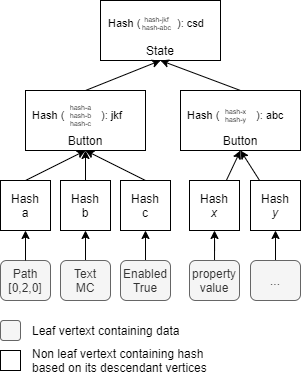
\includegraphics[scale=0.8]{images/merkle-tree-example.png}
\captionof{figure}{An short Merkle tree example based on a widget tree}\label{fig:merkle-tree}
\endgroup

\subsection{How is an inferred model created?}
This research focuses itself on the outcome of the obtain state step as illustrated in figure \ref{fig:obtain-state-graph}, which is the top right part of figure \ref{fig:testar-test-cycle}.

\bigskip
\begingroup
\captionsetup{type=figure}
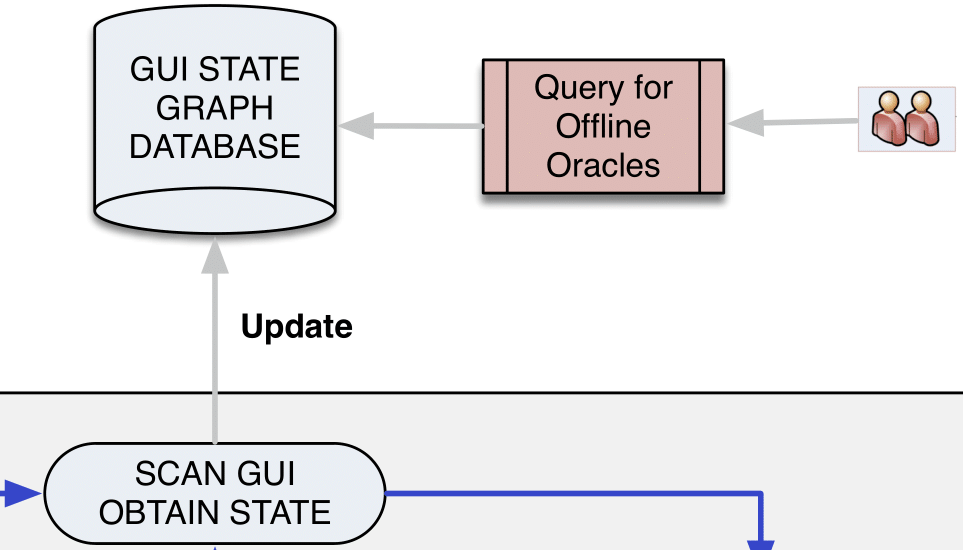
\includegraphics[scale=0.4]{images/obtain-state-graph.png}
\captionof{figure}{The focus of this research proposal \cite{testar-presentation}}\label{fig:obtain-state-graph}
\endgroup

Generating the inferred model starts when \testar start testing the SUT. After an action has been executed successfully, the state of the GUI is sent to the inferred model module. When the state is reached without action, it is marked as the initial state. 

The inferred model module generates the abstract and concrete states and saves those in the model. The model is persisted in the OrientDb database. At last, a deterministic model check is being performed and saved \cite{testar-code}.

\section{State model difference} \label{sec:state-model-difference}
The \verb|StateModel.Difference| package, added by Pastor Ricós\cite{stateDiff}, offers a proof of concept for calculating differences between the inferred state models. For the comparison, the \verb|abstractStateId| is used. 

Pastor Ricós difference algorithm\cite{stateDiff} outputs two classification of changes between two models: added and removed state. Let $A$ be a set of \verb|abstractStateId|s of version 1 of the SUT, and let $B$ be a set of \verb|abstractStateId|s of version 2 of the SUT. The removed states can be written as
\[A-B = \lbrace x | x \in A \wedge x \notin B \rbrace\]
the states that are added can be written as
\[B-A = \lbrace x | x \in B \wedge x \notin A \rbrace\]

\begingroup
\captionsetup{type=figure}
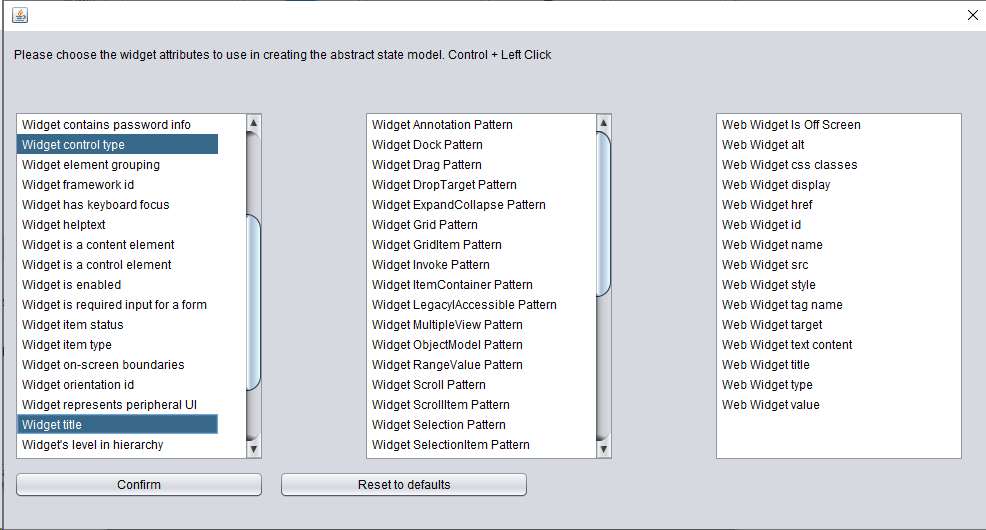
\includegraphics[scale=0.5]{images/attributes-state-model.png}
\captionof{figure}{Select widgets attributes for the abstractStateId}\label{fig:advance}
\endgroup

Using the \verb|abstractStateId| is excellent for the proof of concept and preliminary change detection, 
However, its boolean nature in which state exists or not can result in many 'false' changes. For example, when a widget is moved, the change detection should result in an altered state, not a removed and added state. 

Section \ref{state-identifiers} discussed how identifiers are generated, since the differences are calculated based on the \verb|abstractStateId| selecting the correct widget attributes is vital. Choosing too few attributes could result in conflicting differences like the same actions are removed and added. Choosing too many attributes could trigger a change in even the tiniest detail. Choosing the widget attributes can be done with the 'Advanced' screen under the State model tab. See Figure \ref{fig:advance}.

For the research proposal, an experiment application is created; the two-buttons app. With the two-buttons app, it was possible to experiment with various \testar settings. The application is shown in figures \ref{fig:exp-v1}, \ref{fig:exp-v2} and \ref{fig:exp-v3}. As one can observe, the differences between version 1 and version 2 are the added button with the label 'Hello v2' and between version 2 and 3 the buttons' colour and position. 

\begin{tabularx}{\textwidth}{@{} 
   >{\raggedright\arraybackslash}X
   >{\raggedright\arraybackslash}X  }
    \begingroup
    \captionsetup{type=figure}
    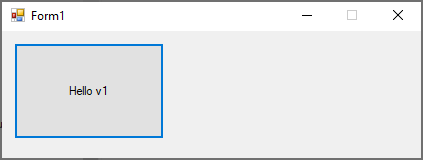
\includegraphics[scale=0.60]{images/exp-v1.png}
    \captionof{figure}{Version 1 of the experiment application}\label{fig:exp-v1}
    \endgroup
    &
    \begingroup
    \captionsetup{type=figure}
    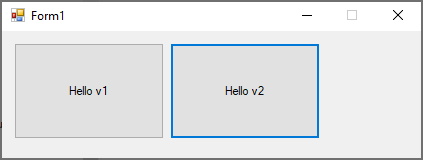
\includegraphics[scale=0.60]{images/exp-v2.png}
    \captionof{figure}{Version 2 of the experiment application}\label{fig:exp-v2}
    \endgroup
    
    \\
    
    \begingroup
    \captionsetup{type=figure}
    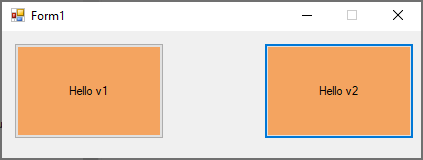
\includegraphics[scale=0.6]{images/exp-v3.png}
    \captionof{figure}{Version 3 of the experiment application}\label{fig:exp-v3}
    \endgroup
\end{tabularx}


However, a different result is displayed when using 'widget title' and 'widget control type' as widget attributes for the abstract states. Namely, the button with the label 'Hello v1' is removed between the first two versions. The buttons labelled 'Hello v1' and 'Hello v2' are added. Between versions 2 and 3, no differences are observed.

This change difference outcome can be explained by the way the proof of concept is working. The widget tree of version 1 contains one button, whereas the widget tree of version 2 contains two buttons. Therefore both the abstract and the concrete identifiers are different for both widget trees. The proof of concept change detection checks whether the abstract identifier of version 1 can be found in version 2, which it cannot, so the state is marked as removed. The state of version 2 can likewise not be found in version 1 so that state is marked as new.

The chosen widget attributes explain the absence of changes between versions 2 and 3. Neither the title nor the control type has changed. Since those attributes were used for the abstract identifier, \testar did not detect a change. 

In section (\ref{research-questions}), the research questions are discussed. Of course, one of the questions will investigate how the change detection algorithm must be implemented. The findings of the two-button app should be considered, and the experiment should be adapted to contain different changes to test on. 

\section{\testar in containers}\label{sec:testar-in-docker}
A recent master thesis by Slomp explains how \testar can be integrated into a \acrfull{ci} environment \cite{thesisSlomp}. Slomp introduced \testar into the world of Docker and container and integrated \testar into an Azure DevOps pipeline. A pipeline is a collection of steps that can automatically build, test and release software. A container bundles all the software, configuration files and libraries together so that an application can run \cite{ms-container}. 

When \testar is being run within the Azure DevOps pipeline, the \testar GUI is not shown. Running \testar is not a problem. However, to analyse the outcome of \testar, the users need to install \testar and have access to the OrientDb database location. 

By moving the code for change detection and visualisation into a stand-alone web application, the user can analyse the outcome on their browser. Since \testar is wrapped into a container, the stand-alone tool will also be wrapped to provide the same infrastructure. Nevertheless, it is up to the IT administrator how they deploy the \testar suite. 

Additionally, to the user's benefit, a \testar developer can also benefit from the application's separation. Changes to either the separate application or \testar can be made without being conflicting with the other. Each tool can focus on one goal, while \testar can focus on testing GUI applications. 
    \newpage
    
    \chapter{Related work}

\todo{make better introduction for related work. }

\subsection{What is a change?} \label{sec:what-is-change}

Not many research papers could be found that define the word change. A clear definition of the word \textit{change} is found in a psychology paper by Rensink \cite{rensink2002change}.

\begin{quote}
    "The word change generally refers to a transformation or modification of something over time. As such, this notion presumes a nonchanging substrate on which changes are imposed. More precisely, change is defined here [the paper] as the transformation over time of a well-defined, enduring structure." (Rensink, 2002, p. 248).
\end{quote}

The definition of the word change can be translated to the language of \testar. The "well-defined, enduring structure" refers to the GUI of the system under test, whereas the "transformation over time" refers to the various version of the SUT. The "something" refers to a part of the GUI that can change like: Widget tree, the state or an action. 

Besides defining the word change, Rensink also describes the differences between changes and differences. A change is a transformation of the same 'something', whether a difference lacks the property of the same something. For example, what are the differences between two distinct SUT, or the same SUT but in two distinct environments or Internet Browsers? A limit to the change detection algorithm is that the SUT needs to be executed in the same environment; otherwise, false-positive changes can occur.

This distinction of definitions between change and differences give the first limit to this research paper's proposed change detection algorithm. The change detection algorithm will give the changes of a SUT, between versions, in the same environment since a different environment can influence the model and therefore influence the outcome of the change detection.

\subsection{What change detection?}


\section{detecting changed by model comp} 

model 

\subsection{Murphy tools}
\todo{After comment resolvement, move Murphy tool from background to this chapter}

GUI driver 

Reference testing GUITAR creates model of current version -> generate test cases... when TC fails -> test failure. 
new features are not failing test cases. 

Browser comparison -> ??

How to compare graphs and visualise them. 

Change visualisation

no much research has been done finding changed in inferred mdoels. There is however a research field that come close to what the research is try to achive, namely cross browser testen. Insted of finding changes between two versions of the same application, with cross browser testing it tries to find differences of the same version but on different browsers.





    \newpage

    \chapter{Research} \label{questions}
In this chapter, the research questions for the thesis are formulated. What research method will be used, and how the questions are being validated.

\section{Context}
The graduation assignment evolves around change detection and visualising the comparison between version of the application under test. The result is an external application that connects to OrientDB and calculates and shows the model comparison. Figure \ref{fig:components-overview} shows the different components involved. The \textit{New Analysis Website} component is the component that is created. Section \ref{sec:components-explained} explained the different components in more detail.

The external application is built as a separate application next to the \testar application. The code that was created by Pastor Ricós (Section \ref{sec:state-model-difference}) and Mulders (Section \ref{inferred-model}) are used as a starting point for the external application. 

\begingroup
\captionsetup{type=figure}
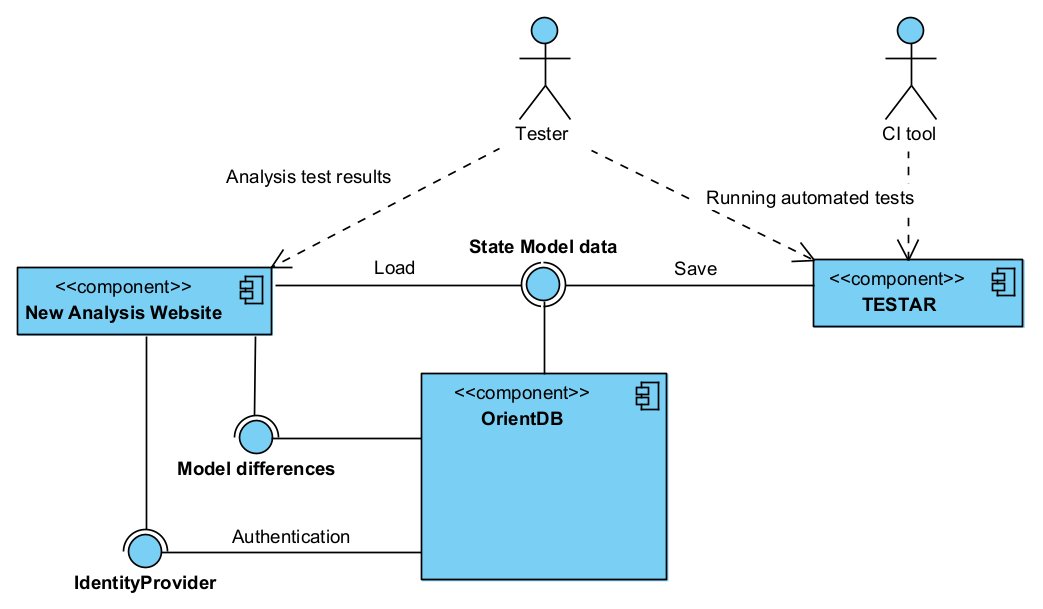
\includegraphics[scale=0.4]{images/3-UML-high-level.png}
\captionof{figure}{Components overview (UML 2.0)}\label{fig:components-overview}
\endgroup

Because change detection is the subject for this graduation assignment, it is assumed that the inferred model generator will generate useful models for change detection. Although the inferred model generator is out-of-scope, it is not ruled out that changes are necessary.

Any automatic learning capabilities are also out-of-scope. A change detection learning capability could be a topic for a future research proposal. Regarding this research proposal, a human will be needed to evaluate the results and outcome of the change detection application.

\section{Research questions} \label{research-questions}
        
The main research question is: \textbf{How can an automated comparison of inferred models help testers finding bugs?}

The main research question is divided into three parts. The first part (\ref{rq:detect-changes}) will research how to detect changes between different versions of the same GUI software (SUT) \cite{testar-todo}. The second part (\ref{rq:diff-visualisation}) will research how to visualise the detected changes. A third Research Question \ref{rq:validation} is dedicated to validating the previous research questions. The research questions are as follows: 


\begin{questions}

    \item How can we set up the change detection as an application written outside of \testar? \label{rq:application-outside-testar}

    \item How to detect changes between two versions of the SUT? \label{rq:detect-changes}
    \begin{questions}
        \item What is change detection, and what do we want to use it for? \label{rq:what-is-change-detection}
        \item Which properties make a model useful for change detection? \label{rq:useful-detection}
        \item Which \testar configuration will generate the useful model? \label{rq:testar-config}
        \item How can we find changes between two models? \label{rq:finding-changes}
    \end{questions}


    
    \item How to visualise the detected differences to the user? \label{rq:diff-visualisation}
    \begin{questions}
        \item What tooling is available to show the result of the change detection? \label{rq:tooling}
        \item How to visualise each change? \label{rq:type-visualisation}
        \item How to generate the shortest set of actions that helps the user to reach the changed state in the SUT? \label{rq:shortest-set}    
    \end{questions}
    
    \item How to validate the results of \ref{rq:detect-changes} and \ref{rq:diff-visualisation}? \label{rq:validation}
    \begin{questions}
        \item What are the requirements for validation applications? \label{rq:req-apps}
        \item Which applications can be used for validation? \label{rq:validation-apps}
    \end{questions}
\end{questions}

\subsection{\ref{rq:application-outside-testar}How can we set up the change detection as an application written outside of \testar?}
\todo{write this section}
extra things had to be done
Industial standards
F-Secure


\subsection{\ref{rq:what-is-change-detection} What is change-detection, and what do we want to use it for?}
To get an answer for \ref{rq:what-is-change-detection}, a literature study will be conducted. The literature study aims to bring an overview of change detection in general and its application in the \testar context. Not only change detection in the GUI but also other change detection methods in the field of Software Engineering, like cross-browser testing. 

\subsection{\ref{rq:useful-detection} Which properties make a model useful for change detection?}
The outcome of \ref{rq:useful-detection} is a list of requirements for the inferred model that are needed to enable change detection. For example, can a non-deterministic state model be used? However, it also includes requirements for the algorithm, like, what are acceptable calculation speeds and how big can a state model be while still complying with the speed requirement? When the set of properties are known, Vaandrager's criteria are used to validate the model \cite{vaandrager}.

\subsection{\ref{rq:testar-config} Which \testar configuration will generate a useful model?}
There are a couple of ways to change the outcome of an inferred model, for example, picking widget attributes for the hash calculation. These configurations can influence the usefulness of the model. The outcome of \ref{rq:useful-detection} should result in a \testar configuration file that configures \testar to generate this useful model. It might be necessary to make code changes in the state model generation or to the identification calculation to implement a Merkle tree approach. Using a Merkle tree could help with comparison to graphs, especially changed in the widget tree. 

A threat of validity for \ref{rq:testar-config} is that every application under test needs its unique configuration. Therefore, it might be wise to look into all widget attributes during the change detection and not take the hash of a state for the comparison. The configuration can be used for tuning the model and the change detection by taking the above approach.

\subsection{\ref{rq:finding-changes} How can we find changes between two models?}
\ref{rq:finding-changes} is the closing question in which the change detection algorithm is coded in Java. In a recent master thesis by Slomp \cite{thesisSlomp}, it is possible to run \testar in a Docker container. As a consequence, \testar can run without a GUI. Therefore the change detection algorithm will run in a separate application, outside the \testar context. The result of the change detection needs to be saved to a data store, preferably the already existing OrientDb database. 

\subsection{\ref{rq:tooling} What tooling is available to show the detected differences?}
Aside from the inferred model, Mulders also created an application to visualise the models. It is essential to state that Mulders did extensive research on which technology fits his needs best. \ref{rq:tooling} will look at the results of Mulders and revalidate whether the libraries are suitable for visualising the differences. 

\subsection{\ref{rq:type-visualisation} How to visualise change?}
\ref{rq:type-visualisation} will look into the execution of the visualisation tool. How can added, removed or altered states in the inferred model be visualised the best? Like \ref{rq:finding-changes} this also includes moving the visualisation tool into its separate application, outside the \testar context. The requirements and GUI proposals will be discussed with the \testar stakeholders. 

\subsection{\ref{rq:shortest-set} How to generate the shortest set of actions that helps the user to reach the changed state in the SUT?}
One of the requirements of the visualisation is showing how to reach the state that has changed. Dijkstra's algorithm \cite{dijkstra1959note} is a well-known algorithm to find the shortest path for a given graph. However, as Goldberg and Harrelson \cite{goldberg2005computing} showed, it is not the most optimal shortest path algorithm, especially with massive graphs. 

\subsection{\ref{rq:req-apps} What are the requirements for validation applications?}
To validate the outcome of the change detection algorithm, we will need to have an application to test it on. The research question will create a set of requirements for the validation application, like multiple versions. The set will be discussed with the supervisors to make sure nothing will be forgotten.

\subsection{\ref{rq:validation-apps} Which applications can be used for validation?}
During development and system testing, the two-button app will be extended and used. Although the app is excellent during the development phase, it is nowhere close to a real-world application. Based on the outcome of \ref{rq:req-apps}, an application needs to be found in order to test the change detection algorithm.

In addition to the application found, F-secure will be asked for feedback on the algorithm and the visualisation. F-Secure is a company based in Finland that provides security solutions to its customers and are currently testing the proof of concept of Pastor Ricós \cite{f-secure}.

With the combination of real-world application and the feedback from F-Secure, biased towards a single point of view for the algorithm will be minimized. 
    \newpage    
    
    \documentclass{ou-report-vaf}

% Dit template is gemaakt door P.J. Molijn in het kader van zijn afstuderen aan de OU in 2014.
% Waarvoor hartelijk dank.
% Minieme maar belangrijke wijzigingen zijn aangebracht door E.M. van Doorn
% Het template is versimpeld door Sylvia Stuurman, 2019.
% Het template is aangepast voor de ba informatica door Harrie Passier, Tanja Vos en Pekka Aho 2020 
% Het tamplate is aangepast met nieuwe huisstyle door Rick Neeft, 2021
% TODO command toegevoegd, 2022

\def\mytitle{How can automated comparison of inferred models help testers finding bugs?}
\def\myauthor{Rick Neeft}
\def\myStudentId{851829973}
\def\myPresentationDate{T.B.D. 2022}

\newcommand{\testar}{\textsc{testar }}
\newcommand{\testarnet}{\textsc{testar .NET }}

\begin{document}

    \pagenumbering{roman}

    % Elements of the thesis
    %%%% TITLE PAGE %%%%%%%
% front cover should be a empty as possible. Title (subtitle) - Name - student Id and thesis presentation date

%to prevent that the title page will be referred as page 1, 
%which will give the warning that there is a page 1 twice.

\pagestyle{plain}

\begin{titlepage}
    \newgeometry{right=100pt,left=58.8pt}

    \pagecolor{ou-light-gray}
    \afterpage{\nopagecolor}
    
    %% Insert the OU logo at the top right corner of the page
    %% PowerPoint contains 84 pt margin in picture
    \begin{tikzpicture}[remember picture,overlay]
                \node at (current page.north east)[anchor=north east,inner sep=58.8pt]{
            
\includegraphics[scale=0.5]{images/ou-text-logo.png}
        };
    \end{tikzpicture}
    
    %% Extra whitespace at the top.
    \vspace*{5\bigskipamount}
    
    %% add title without hypens
    \nohyphens{{\color{ou-red}\Huge\bf \mytitle}}
     
    \bigskip
    %{\large subtitle, if any}
    
    %\bigskip \bigskip
    %by
    \bigskip \bigskip
    
    {\Large\bf \myauthor}\\
    {\large\myStudentId}
    
    {\myPresentationDate}
    
\end{titlepage}

% reset geometry since we changed them for the title page
\newgeometry{right=0.875in,left=.875in}

%%%% END TITLE PAGE %%%%%%%

    % Page 2 must be left blank
    \myemptypage
    
    % Page 3 contains all compulsory data.
    \addcontentsline{toc}{chapter}{Compulsory data}

\myauthor, \myStudentId\\
\textbf{\mytitle}\\
\myPresentationDate
\vspace*{\fill}

Open University of the Netherlands, Faculty of Science\\
Master's Programme in Software Engineering\\
\\
Graduation committee

Chair: Prof. Dr. Tanja E.J. Vos\\
Primary supervisor: Dr. Pekka Aho\\
Seconday supervisor: Fernando Pastor Ricós

Course code: IM9906
\newpage
    
    % Acknowledgements
    \chapter*{Acknowledgements}
\addcontentsline{toc}{chapter}{Acknowledgements}

I want to thank my supervisors, Pekka Aho, Fernando Pastor Ricós and Tanja Vos, for the opportunity and support of my graduation project. The weekly meeting and feedback were always inspiring and gave me good directions on what to do. I am grateful for allowing me to develop the application in C\#. Besides academic learning, using C\# and Blazor is extremely helpful in my day-to-day career.

Thanks to WithSecure, especially Joona Oikarinen and Tatu Aalto, for their input and feedback regarding the Analysis website and the docker setup.

I want to thank my wife for her support and for allowing me to sit in our home office for countless hours. 

Thank you to my family, and special thanks to my mother, who always supported me and pushed me to achieve my life goals. 

Last but not least, I want to thank my employer, VECOZO, for providing me with time and resources to finish my Masters. 

Rick Neeft\\
\myPresentationDate
    %\myemptypage
    
    % Table of contents
    \begingroup
        \hypersetup{linkcolor=black}
        \tableofcontents
    \endgroup
    \newpage
    
    % Summary
    \chapter*{Summary}
\addcontentsline{toc}{chapter}{Summary}
lorem ipsum blah blah yadda yadda yadda
    %\newpage
    
    % the content of the thesis
    \pagenumbering{arabic}
    
    \chapter{Introduction} \label{introduction}
    
Regression testing is considered a good practice when testing new software versions before being released to the general public. 
However, due to shortened release cycles, the time to market has decreased drastically. As a result, software test teams have less time to test all new software features, let alone try all other elements to prevent unwanted side effects \cite{rapid-release-cycle-issues}.
The research proposed aims to apply change detection between two versions of the GUI of the system under test. 

This section introduces the proposed research discussing the background and context, followed by the research problem, research aims, research questions and why this research is important.

\section{Background}
The TESTAR tool solves a significant obstacle when it comes to testing the GUI. With TESTAR, the tester can automatically start testing the GUI without any upfront scripts. TESTAR automatically generates and executes test sequences based on elements derived from the GUI \cite{VosAho2021}. In recent master graduation assignments, TESTAR has been extended with an inferred model generation module \cite{thesisMulders}, and it became easier to integrate TESTAR in build and release pipelines in a DevOps environment \cite{thesisSlomp}. Those two additions make it easier to run TESTAR upon each source code integration and retrieving an inferred model about the GUI. In a proof of concept, two inferred models are compared to get changes between versions of the SUT \cite{stateDiff}.

Some companies might write down changes of the software in a changelog. However, some changelogs might not be complete and unwanted side effects might be missing entirely. Comparing two inferred models shows all the changes between versions of a SUT, even the unwanted ones.

\section{Research problem}
Although the proof of concept for change detection is a good start, it lacks some basic functionality. For example, it compares calculated abstract hashes with each other. As a result, even the slightest change in GUI results in a removed and added state between versions.

In addition to change detection, the change visualisation does not use the build-in visualisation tool. The proof of concept generates an HTML-based report, making it difficult to see where the change can be found and which steps the tester needs to take to navigate to the changed state in the software.

\section{The aim of the research}
The research aims to apply change detection on the inferred model created with the automated GUI testing tool TESTAR and research whether the outcome is helping testers finding bugs quicker. The main research questions are:

\begin{questions}
    \item How to detect changes between two versions of the SUT?
	\item How to visualise the detected differences to the user? 
\item How to validate the results of \ref{rq:detect-changes} and \ref{rq:diff-visualisation}?
\end{questions}

\section{Scope}
The scope of the research is change detection in GUI inferred models created by TESTAR. Researching how to make models and making significant changes to the creation of models are omitted. However, tweaking the model generation, like adding data that is not saved at the moment, and configuring TESTAR to create a good model, are in scope.

\section{Contribution}
When change detection is available in TESTAR, it becomes easy for testers to run the comparison in a continuous integration environment and receive an overview of the changes found in an updated version of the software.

As a side effect, the comparison and visualisation solutions can run outside the context of TESTAR and can be deployed to a docker environment.

\section{Document outline}
This research proposal is structured as follows. In section \ref{intoduction} the context, aim and objectives for this research proposal are introduced, together with the limitations for the expected outcome. Section \ref{background} describes the background of this proposal and contains knowledge that is available but might not be known by the readers. Section \ref{releatedWork} includes an overview of the material that can be seen as a direct foundation for this proposal or work that influences the expected outcome. Section \ref{questions} formulates the research questions for the thesis. The last section \ref{planning} will outline the chosen approach and planning for the graduation assignment.
    \newpage
    
    \chapter{Background} \label{background}

\todo{make better introduction for the chapter. }

This section describes the background of this proposal and contains information that is available but might not be known by students and readers. 

\section{Introduction into GUI Testing}
Ever since the first line of software is written, testers are testing its workings. While in the early day of software, the \acrfull{ui} was mainly terminals based or a set of blinking LEDs \cite{altair8800} \footnote{For example the ALTAIR 8800 computer \cite{altair8800}}, today we have an ever-increasing amount of \acrfull{gui} applications. Testings a GUI application is labour intensive and costs a lot of money \cite{gui-history}.

Initially, testers were using \acrfull{cr} software to automate their work. A tester would record a test scenario into the CR software, and then the CR software will execute the test case when needed. Using CR software, the time required to retest software decreases; however, the big downside is that when software changes, so must the recorded scripts \cite{gui-history}.

Then came \acrfull{mbgt}. With MBGT, the GUI elements and behaviour are abstracted on a higher level. The created models are used to generate abstract test cases. Those abstract test cases need to be mapped or transformed to get concrete test cases that are executed on the SUT. The downside of MBGT is the effort required to create the models and the need to have formal modelling expertise. Formal modelling expertise is not needed with the latest evolution in test automation: model inference. 

The \emph{model inference}, also known as model extraction and GUI Ripping \cite{gui-ripping}, is the current state-of-the-art approach to automate GUI testing \cite{gui-history}. Inferred models are state graphs based on the GUI of the SUT. There are two ways to generate inferred models; the first is a static approach where the source code of the  SUT is used to create a GUI model. The second is a dynamic approach where the GUI state is captured and extracted while being executed. 

The static approach has several downsides. First, the source code must be available, which is not always the case and secondly, it is challenging to capture behaviour based on the GUI source code. For example, with HTML, it is easy to generate a model; however, its behaviour is either in Javascript or server code.  It is possible to overcome those stumbling blocks by executing the SUT.
    
As for the Dynamic approach, it captures the model during test execution. The automated test tool interacts with the SUT in a scriptless and random way. This random scriptless approach is called \emph{Monkey testing}. Usually, test monkeys have no idea in which state the SUT is in and what type of input is allowed. It is therefore essential to make the test monkey smarter. A "smart test monkey" can be achieved by making them "see" the UI elements (Section \ref{data-retrieval}). Section \ref{testar-testauto} will give more details about how \testar is using smart test monkeys.

\section{What is \testar?} \label{what-is-testar}
\testar - or TEST* - is an automated software testing tool for the GUI level \cite{testar-about}. \testar started within the context of the \acrfull{fittest} project. \testar is open-source, the source code is published on GitHub \footnote{ \url{https://github.com/testartool/testar\_dev}}. A screenshot of the \testar tool is displayed in Figure \ref{fig:testar}.

\bigskip
\begingroup
\captionsetup{type=figure}
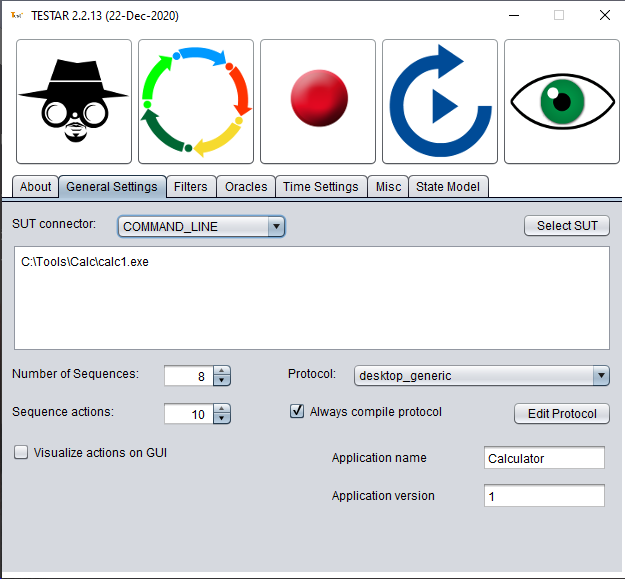
\includegraphics[scale=0.5]{images/testar.png}
\captionof{figure}{Screenshot of the \testar tool}\label{fig:testar}
\endgroup

\testar has several \emph{execution modes} in which it interacts with the SUT \cite{testar-manual}. From left to right, in figure \ref{fig:testar}, those are Spy, Generate, Record, Replay and View mode.

The \emph{Spy} mode allows the user to inspect a SUT and analyse how \testar is interpreting the widgets on the screen. Figure \ref{fig:calc-spy} shows the Windows calculator in spy mode. Dots on the GUI indicate actions that \testar could execute to interact with the SUT. Furthermore, within \testar, it is possible to filter out actions. Then, \testar will not execute those actions. The filtered actions are marked with a grey-coloured dot. A list with properties about the widget is shown when hovering, as well as a unique identifier of the current \emph{state}, more information about the state and the unique identifier can be found at section \ref{gui-state}.\par

\bigskip
\begingroup
\captionsetup{type=figure}
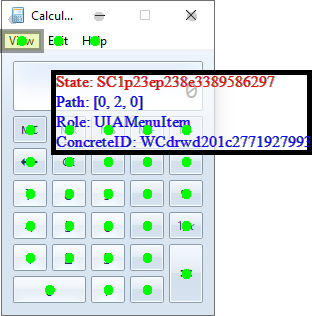
\includegraphics{images/calc-state.png}
\captionof{figure}{Screenshot of the Calculator with \testar Spy}\label{fig:calc-spy}
\endgroup

In the \emph{Generate} mode, \testar will start testing the specified system. Section \ref{testar-testauto} gives more details about \testar test automation.

The \emph{Record} mode allows a tester to record a test sequence manually. In the \emph{Replay} mode, existing test execution can be re-executed and lastly, the \emph{View} mode allows existing test executions to be viewed.

\newpage
\section{TEST automation} \label{testar-testauto}
\testar works without test scripts. Instead, it uses GUI Ripping and Monkey testing techniques. \emph{GUI Ripping}, first introduced by Memon et al. \cite{gui-ripping}, is a process to obtain the GUI's structure and execution behaviour automatically. As for \emph{Monkey testing}, it is a process in which decisions (interactions with the GUI) are randomly made. Section \ref{data-retrieval} will give more insights into GUI Ripping.

\testar is using a flow to execute tests on the SUT. This flow is as follows:
\begin{samepage}
\begin{enumerate}
    \item Start the SUT
    \item Scan the GUI and obtain the state (Section \ref{gui-state})
    \item Finding and selecting an action to execute
    \item Evaluate state with a test oracle (Section \ref{test-oracles})
    \item Stop the SUT when no actions are left to be executed or restart the SUT when more sequences are required.
\end{enumerate}
\end{samepage}

\bigskip
\begingroup
\captionsetup{type=figure}
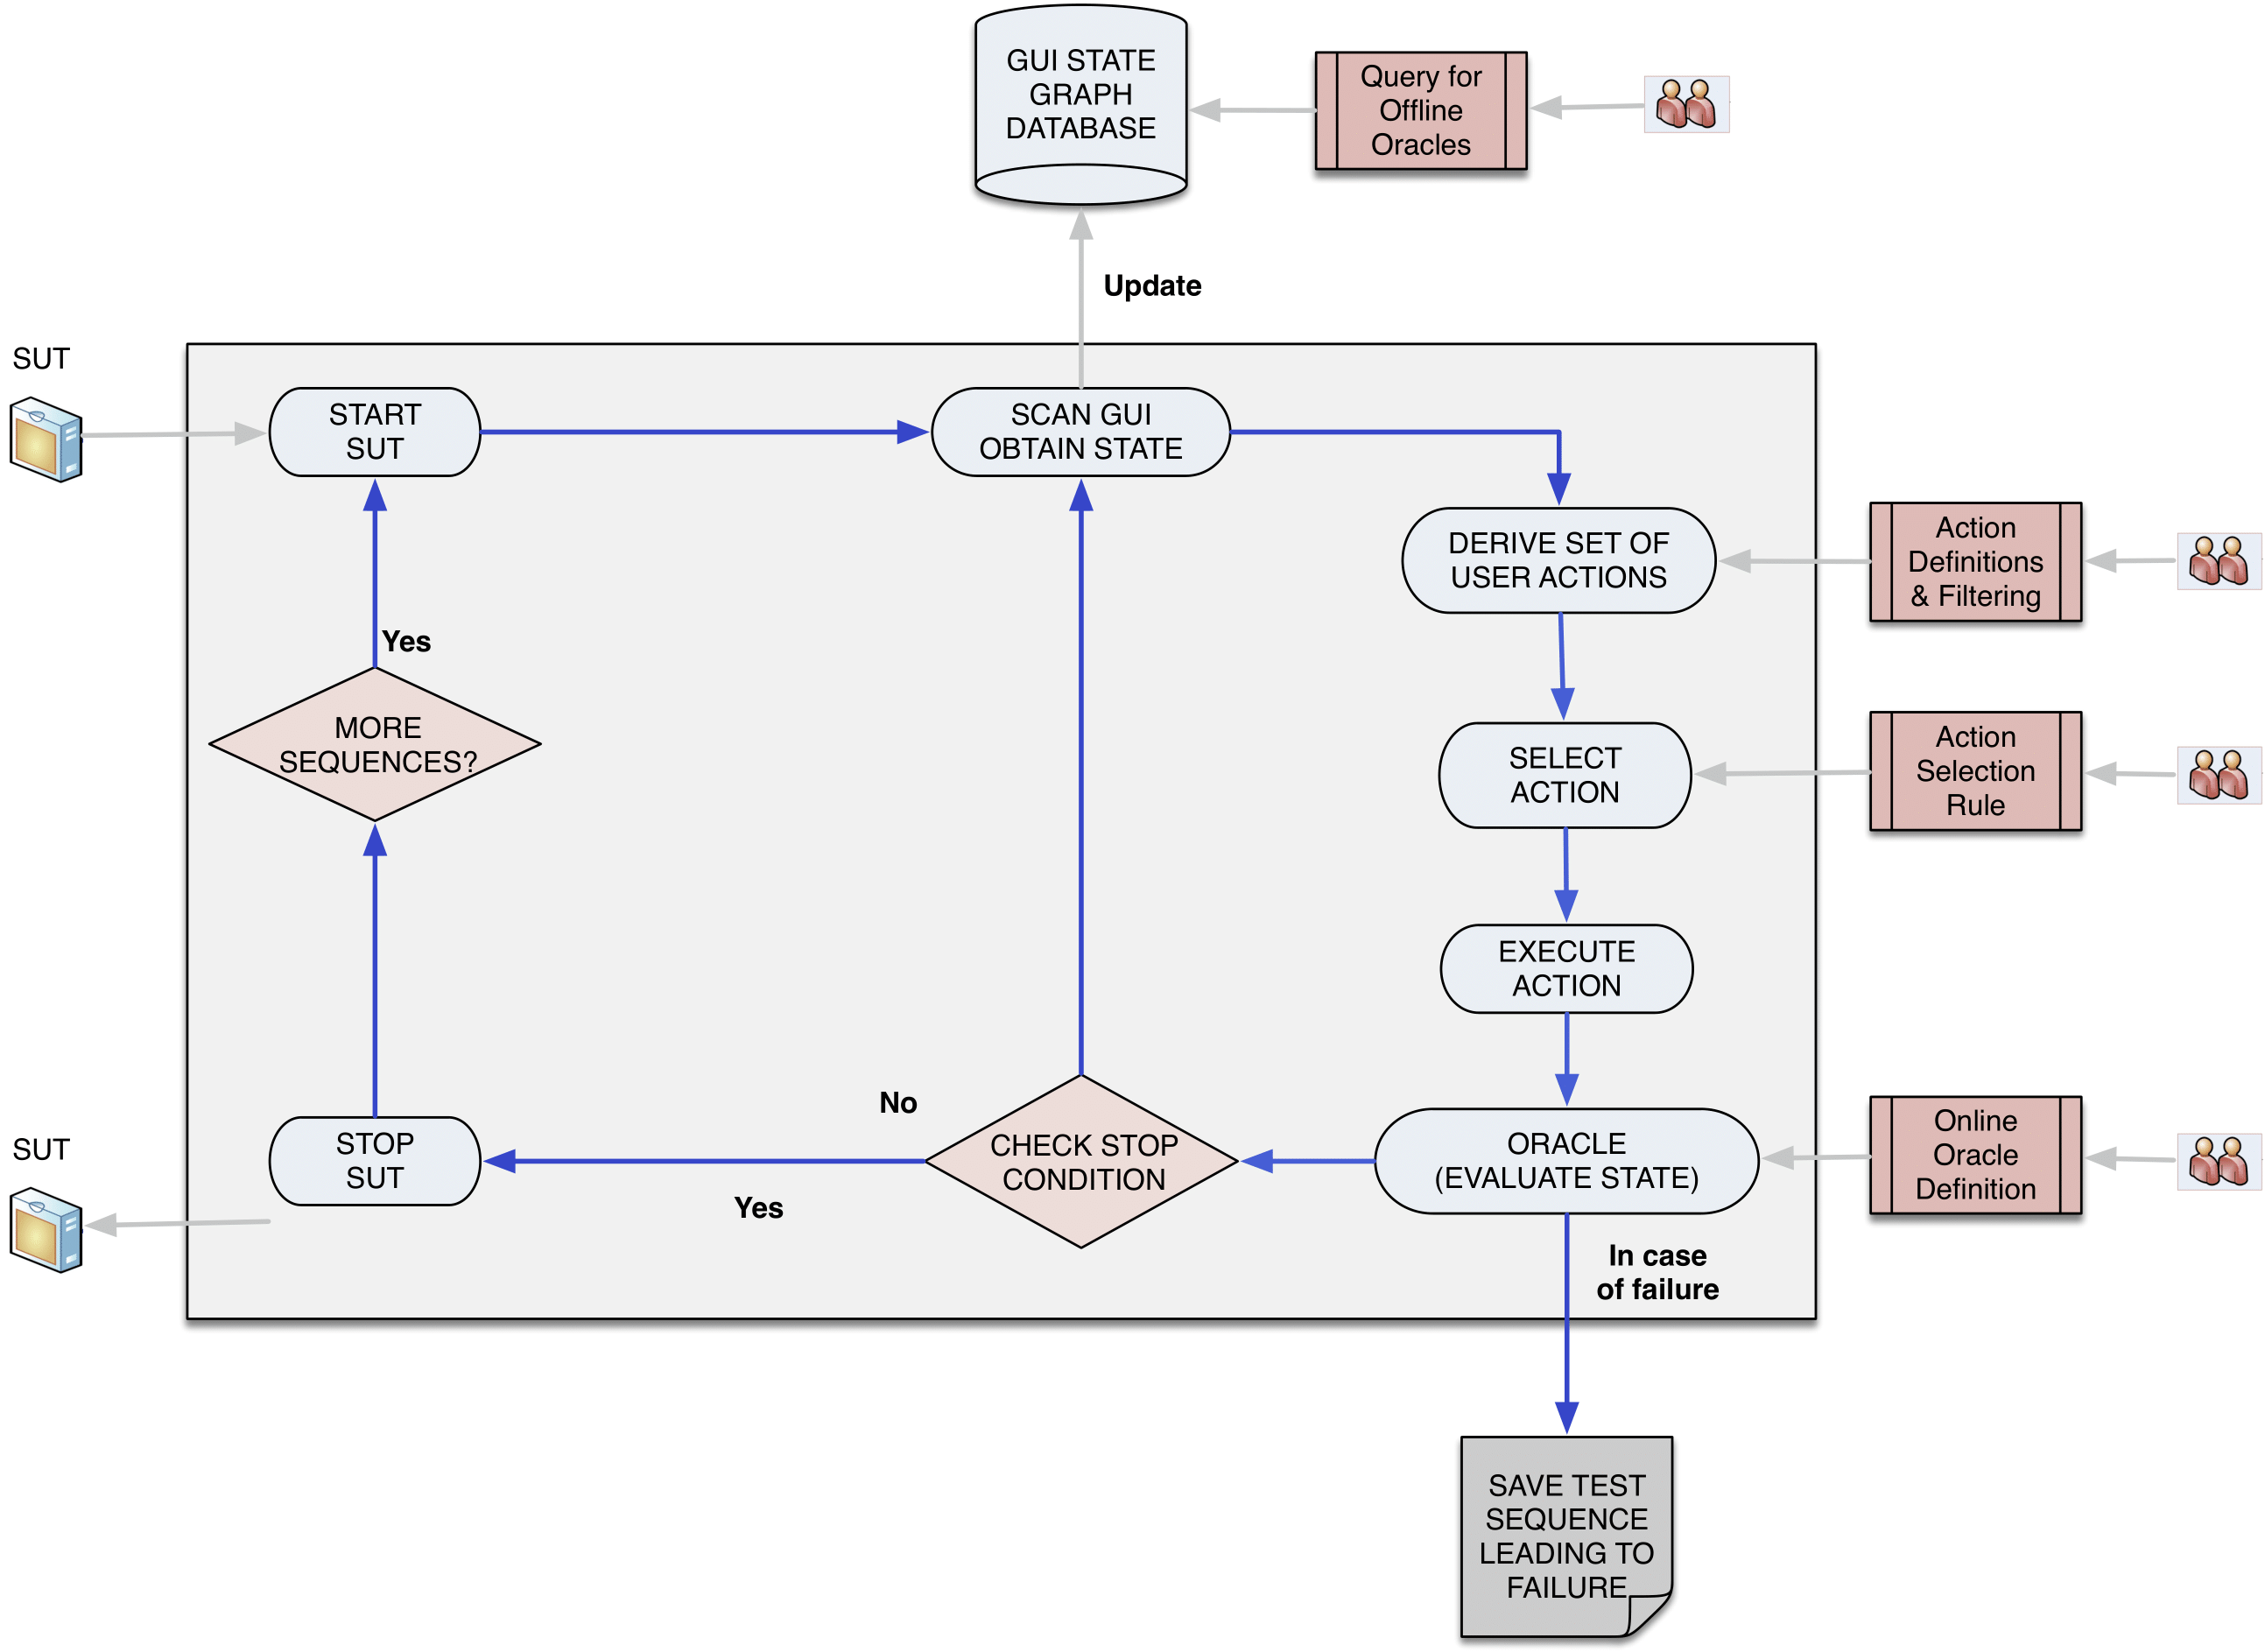
\includegraphics[scale=0.36]{images/testar-test-cycle.png}
\captionof{figure}{\testar test cycle \cite{VosAho2021}}\label{fig:testar-test-cycle}
\endgroup

Figure \ref{fig:testar-test-cycle} shows the flow graphically \cite{VosAho2021}. The test specialist needs to provide SUT details to \testar, like which actions should not be executed, and devise a mechanism that defines which SUT behaviour is correct and which is not, named a test oracle (Section \ref{test-oracles}). 

\section{How is the SUT tested} \label{test-oracles}
When software is tested, a method is needed to check the correct behaviour of the SUT. The method of checking is formally known as a \emph{test oracle} \cite{testOracles}. 

Outside the \testar context, an example of a test oracle could be an \emph{assertion} in software code. An assertion is a boolean expression created in a program by a software developer which checks the program's behaviour during run-time \cite{barr2014oracle}. Assertions can also be used in unit tests as displayed below on Listing \ref{code:assert}. 

\begin{lstlisting}[language=Java, caption=Example assertion, label=code:assert]
@Test
public void testAdd(){
    Calculator sut = new Calculator();

    int expected = 3;
    int actual = sut.Add(1,2);

    Assert.assertEquals(expected, actual);
}
\end{lstlisting}

\testar comes with some test oracles out-of-the-box. Without any configuration, \testar will recognize crashes and unresponsiveness. It is also able to validate the GUI state with suspicious text. For example, a test sequence will fail when the title of a widget contains the word 'exception'. The input for the suspicious text is a regular expression that can be adjusted by the \testar user \cite{VosAho2021}. 

\subsection{Online and Offline Test oracles}
Test oracles come in two variants, \emph{online} or \emph{on-the-fly} test oracles and \emph{offline} test oracles \cite{VosAho2021}. With online test oracles, the state under test is being asserted for any anomalies during test execution. For example,  an online test oracle inspects the URL to check for any information being exposed in the query string. Offline test oracles will look into stored data - like logs - to find anomalies after test execution. For example, offline test oracles can inspect all the visited URLs to check for any exposed information in the query strings.

The two test oracle variants are complementary to each other and can run side by side. However, each variant comes with its strengths and weaknesses. The online test oracle takes up computation time because it inspects the state during test execution. This inspection of state slows down the test execution and may become an issue with time-critical SUTs. On the other hand, some issues - like the SUT becoming unresponsive - can only be checked during test execution. An offline test oracle is inspecting the gathered data after test execution has finished. Especially with larger data sets, this can become helpful. Inspecting the data may run in parallel, which can speed up the test oracle. Additionally, when developers create new offline test oracles, they can inspect the recorded data instead of executing a new test run \cite{de2019offline}.

\section{How is data retrieved} \label{data-retrieval}

Section \ref{testar-testauto} discussed how \testar is using GUI ripping to obtain the GUI's structure. A GUI consists of a non-empty set of UI components, known as \emph{widgets}. Examples of widgets are Windows or buttons; more examples can be found in Table \ref{tables:widgets} \cite{VosAho2021}. 

\begingroup
\captionsetup{type=table}
\begin{tabularx}{\textwidth}{ 
  | >{\raggedright\arraybackslash}X 
  | >{\raggedright\arraybackslash}X 
  | >{\raggedright\arraybackslash}X | }
    \hline
    Windows & Menus & Controls \\
    \hline
    \hline
    main windows & menu bars & buttons \\
    child windows & dropdown menus & textboxes \\
    popup windows & context-aware menus & links \\
    && radio buttons \\
    && checkboxes\\
    && dropdown select boxes\\
    && sliders\\
    && tabs\\
    && scrollbars \\
    \hline
\end{tabularx}
\captionof{table}{Example of GUI widgets \cite{VosAho2021}}\label{tables:widgets}
\endgroup

The widgets are structured hierarchically in a \emph{widget tree}. Each node in the tree is a widget with its related properties, such as the title, position and role. In figure \ref{fig:widget-tree} a compact widget tree is shown for the calculator. 

\bigskip
\begingroup
\captionsetup{type=figure}
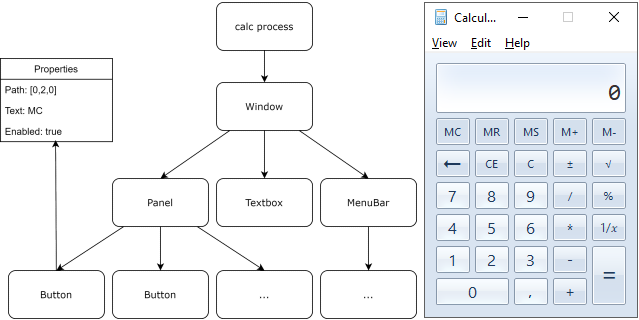
\includegraphics[scale=0.7]{images/calc-tree.png}
\captionof{figure}{A compact version of a widget tree for the calculator.}\label{fig:widget-tree}
\endgroup

\section{Widget data API}

In order to retrieve data from a SUT, \testar is making use of external APIs to access widgets that are part of the GUI \cite{thesisMulders}. \testar is using three different APIs.

In order to test a desktop application, \testar makes use of the Windows Automation API. The purpose of the Windows Automation API is to expose rich information about UI elements\cite{win-api-info}. For web applications, \testar uses Selenium Chromedriver. The Chromedriver is a tool for automated testing. It provides capabilities for navigating through web pages, user input, and JavaScript execution \cite{chrome-driver-info}. The latest API that \testar is using is Appium. Appium is a test automation tool for native, mobile web, and hybrid applications on iOS mobile, Android mobile, and Windows platforms \cite{appium-info}.

\section{GUI State} \label{gui-state}
In the previous sections, the widget tree is discussed and how the widgets are retrieved. In the widget tree, all the GUI elements with their properties are captured. The widget tree represents the state of the GUI when it has stopped executing any action. The GUI is at 'rest'. When an action is executed, the GUI can change, going to a new state. In figure \ref{fig:state-actions} the state change is represented in a small graph. 
\bigskip
\begingroup
\captionsetup{type=figure}
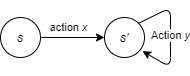
\includegraphics{images/state-action.png}
\captionof{figure}{An graph with two states and two actions.}\label{fig:state-actions}
\endgroup

The graph is a directed graph since every action changes the GUI from one state to the other. An action may lead to the same state, see figure \ref{fig:state-actions} action \textit{y}. However, that would mean that the action does not do anything or \testar does not indicate a change. For example, the GUI changes but the property corresponding to the change is not included in the widget tree.

The universe of states and actions of the SUT's GUI makes up an inferred model. More information about the inferred model and how they are created can be found in section \ref{inferred-model}.

\section{How is data persisted}

\testar is using a database to store and retrieve state model data. Gier and Kager investigated which data storing solution would be beneficial to \testar \cite{GierKager}. The data solution must comply with six requirements. Generally speaking, the requirements were as follows: an open-source graph database with a straightforward query mechanism. The conclusion was that OrientDB was the best solution that met all the requirements.

\begin{samepage}
OrientDB is a Multi-Model NoSQL \acrfull{dbms} that combines four models \cite{orientDbModeling}:

\begin{itemize}
    \item \hyperlink{db:key-value}{Key/Value}
    \item \hyperlink{db:document}{Document}
    \item \hyperlink{db:graph}{Graph}
    \item \hyperlink{db:object}{Object}
\end{itemize}
\end{samepage}

A \hypertarget{db:key-value}{\emph{Key/Value}} is the simplest model and allows storing information (value) that is accessible with a key. Key/Values can be grouped into \textit{buckets}. However, OrientDB supports richer models in the form of document and graph elements.

A \hypertarget{db:document}{\emph{document}} is a schema-less set of key/value pairs. The \emph{key} allows access to the corresponding value. OrientDB allows the developer to store documents into \emph{clusters}. Relations between document are either embedded into other document or \emph{linked} to each other. Someone familiar with relational databases can view a cluster as tables, a document as the row and the key/value pairs are columns.

The \hypertarget{db:graph}{\emph{graph}} is a model consisting of \emph{Vertices} and \emph{Edges}. Vertices are the nodes in the graph, and the edge is the link between those nodes. In \testar terminology, a vertex represents state, and the edge is an 'action' from one state to the next. A Vertex consists of three elements: a unique identifier, a set with incoming Edges and outgoing Edges. An edge consists of four elements: a unique identifier, an incoming vertex (\emph{head}), an outgoing vertex (\emph{tail}) and a label that describes the relationship between the head and tail vertex.\par

The last model is the \hypertarget{db:object}{\emph{object}} that supports inheritance, like in the Object-Oriented programming paradigm.\par

Despite being a NoSQL database, OrientDB does support SQL as a query language \cite{sql-lang} albeit that it does not support all SQL statements. The majority of developers have experience with SQL \cite{sql-stats}, and as a result, new developers and students can start querying the \testar data and start expanding its features.\par

In addition to \testar, other applications can query the state model data in the OrientDB database as well. For example, developers and students can create external tools for a single purpose, like a state model difference application. When building external tools, the \testar application can be kept small and focus upon one objective: testing GUI applications. 

\section{The Murphy tools} \label{murphy-tools}

\todo{This section should go to chapter 3, leaving it here until comment is resolved}

F-Secure, a security software company, based in Finland, developed the Murphy tool \cite{aho2013industrial}. With the Murphy tool, it was possible to automatically extract models from the GUI and use them for GUI testing. The goal of the Murphy tool is to find as many states of a GUI as possible. Users can customise the Murphy scripts to direct the tool to particular cases. 

Like \testar, Murphy creates a directed graph of the GUI under test. Each vertex of the graph is a state of the GUI represented by a screenshot of the GUI. Each edge is an action that the user could perform. 

Like \testar, Murphy is a platform-independent test tool. To accomplish that, Murphy uses various drivers. A driver recognises elements and windows of the GUI under test. One of the drivers uses the 'tab' key to enumerate UI elements. 

While Murphy is crawling the GUI it is making screenshots of the GUI. Besides that, the screenshots represent the state in the graph; they are used to detect changes between different versions of the SUT. 

\section{Inferred model} \label{inferred-model}
The master thesis by Mulders had two significant outcomes. The first is an inferred model module, and the second is the visualisation of the inferred models \cite{thesisMulders}. The visualisation module is a web-based application that shows the inferred model with screenshots and properties. Although the visualisation module will be required when we want to visualise the results of the change-detection software, it is not necessary to go into depth in this document. This section will discuss what an inferred model is and how they are generated. 

The GUI state was discussed in section \ref{gui-state}. The section ended with the sentence that the universe of states and actions of the SUT's GUI makes up the inferred model. The inferred model is a directed graph showing the GUI-state of the application and the transactions between states. The vertex of the graph represents the GUI-state. Each vertex has a set of incoming and outgoing edges, called the actions. 

Figure \ref{fig:state-model} shows the result of the inferred model in the visualisation module.

\bigskip
\begingroup
\captionsetup{type=figure}
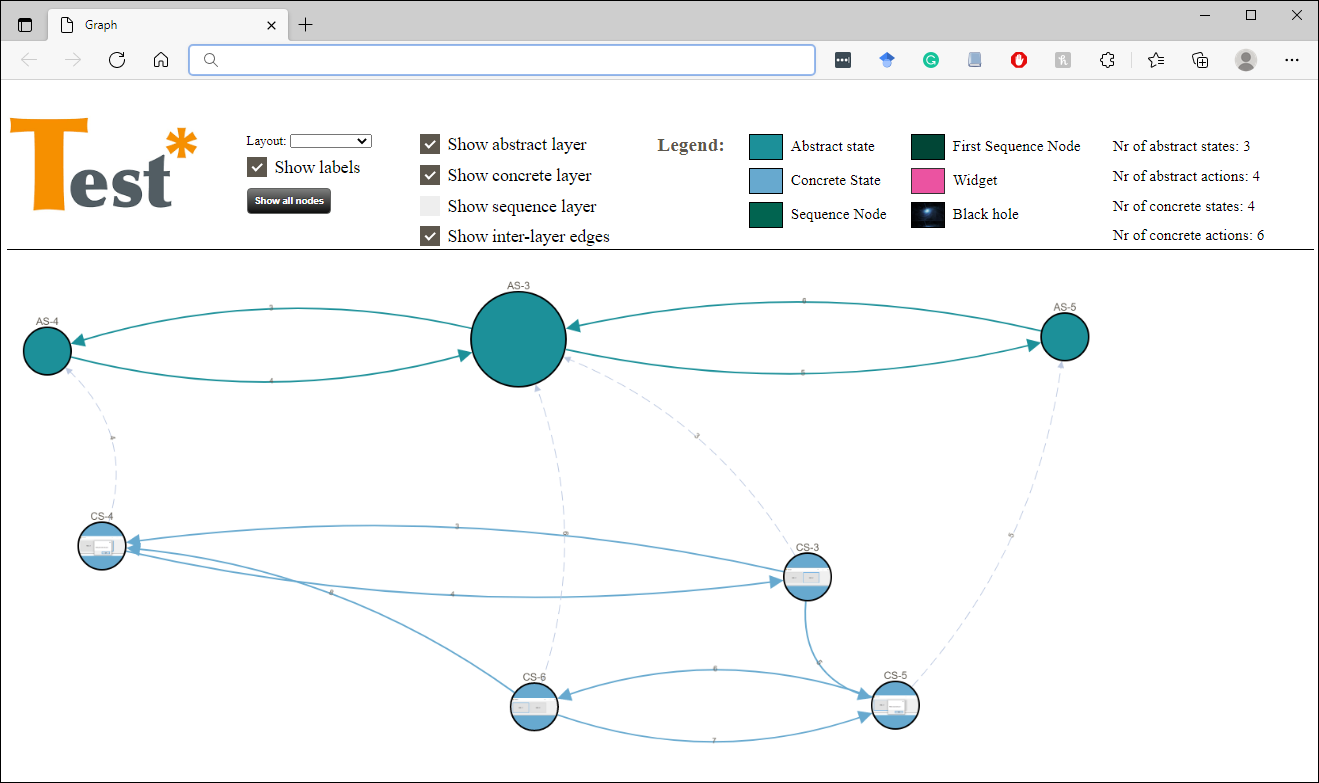
\includegraphics[scale=0.38]{images/state-model.png}
\captionof{figure}{an inferred model in the visualisation application}\label{fig:state-model}
\endgroup

In figure \ref{fig:state-model} two models can be observed. The first model, indicated by the AS text, shows the abstract model. The second, indicated by the CS text, shows the concrete GUI states. 

\subsection{Concrete model}
The concrete model contains all the data that could be retrieved from the GUI. The identification key uses a hash calculated over all the properties. Aside from the widget's properties, the concrete models also contain a screenshot of the GUI for each state \cite{thesisMulders}.

Figure \ref{fig:concrete-node} shows an example of a node in the concrete model. Upon selecting a node, the properties of the node show, including the screenshot taken during the test. The grey dotted line, indicated with the letter 'a', shows the connection with the abstract node, see section \ref{abstract-model} and figure \ref{fig:abstract-model} for more details. The two outgoing edges, indicated with the letter 'b', shows the two actions available in this state. The incoming edge, indicated with the letter 'c', shows how the state was reached. 

\bigskip
\begingroup
\captionsetup{type=figure}
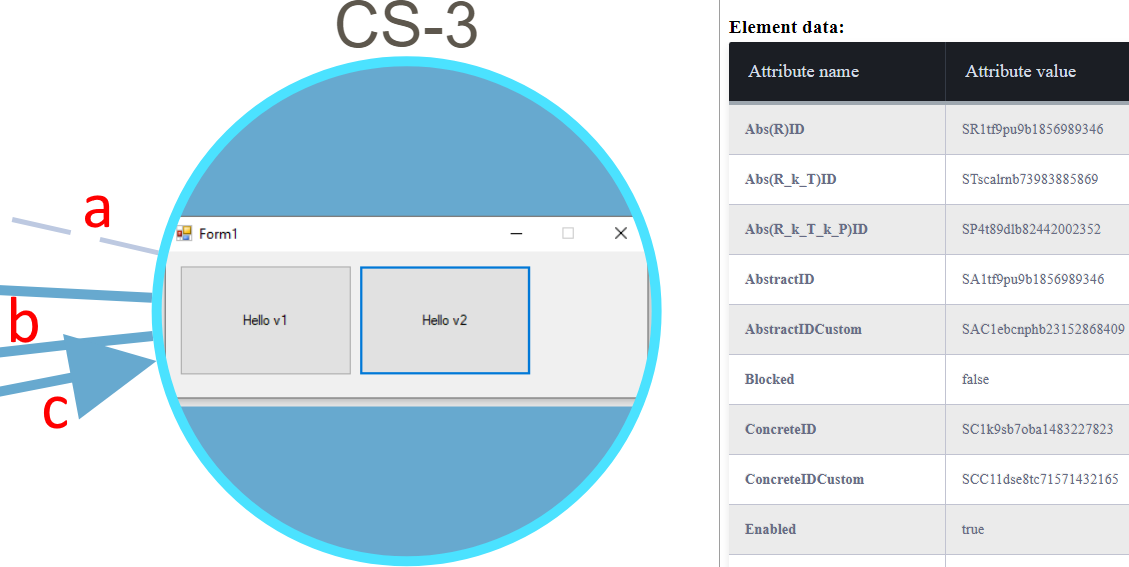
\includegraphics[scale=0.5]{images/concrete-model.png}
\captionof{figure}{A node from the concrete model}\label{fig:concrete-node}
\endgroup

\newpage
\subsection{Abstract model} \label{abstract-model}
Since the concrete models contain all the data from a GUI-state, they can become quite large.  Therefore an abstract state model is made \cite{thesisMulders}. Figure \ref{fig:abstract-model} shows an example of such a abstract node. The grey lines (from CS-3, CS-6 to AS-3) indicates which concrete states are abstracted. The properties of the abstract node are displayed, what the identifier is and which concrete state(s) it represents.

\bigskip
\begingroup
\captionsetup{type=figure}
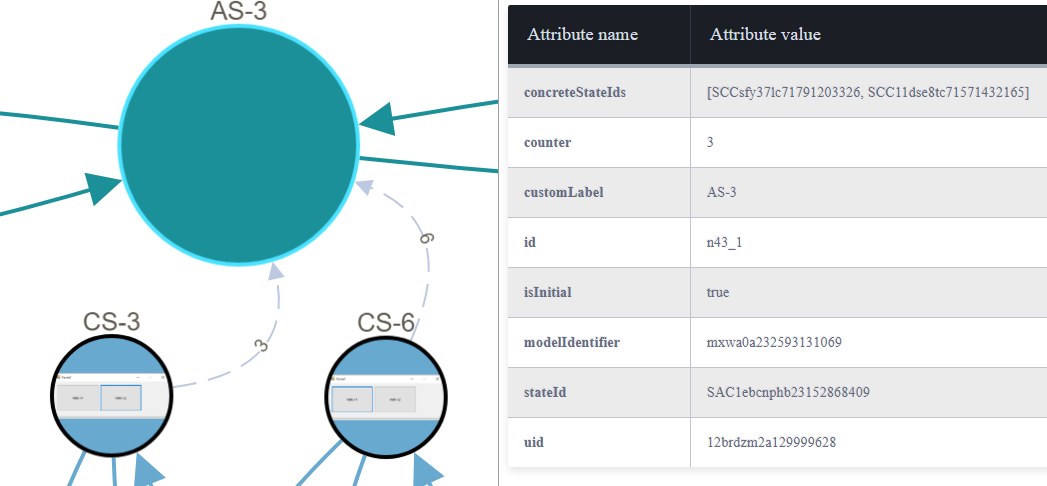
\includegraphics[scale=0.5]{images/abstract-model.png}
\captionof{figure}{A node from the abstract model}\label{fig:abstract-model}
\endgroup

\subsection{State identifiers} \label{state-identifiers}
Every state must have a unique id for identification. The identifier is calculated with the data from the widget tree. 

\testar uses a hashing algorithm that works as follows: the widgets' properties are concatenated and hashed. The outcome will be used as the identifier for a widget. The hashes from the widget in the widget tree are then combined and hashed to create an identifier for the GUI state \cite{VosAho2021}. The \testar's algorithm is similar to how a Merkle tree works, more information can be found at section \ref{merkle-tree}.

To identify the state (and actions), \testar calculates two state identifiers; an abstract and concrete state identifier. For the concrete state identifier, all the properties of a widget are used. For the abstract identifier, a subset of the properties is used. It is configurable which properties are used for the abstract identifier. By default the properties \textit{role}, \textit{title}, \textit{position} and \textit{enabled} are utilised \cite{VosAho2021, thesisMulders}.

When running \testar, it is possible to configure which widget properties should be used for the abstract state identifier. Figure \ref{fig:advance} shows the selection dialogue in which the user can select the properties for the abstract identifier.

\section{Merkle tree} \label{merkle-tree}
A Merkle tree is a hash tree data structure where a hash can identify each vertex. \cite{merkle-tree} The cryptographic hash is calculated by taking the hashes of the descendant vertices, combining them, and calculating a new hash from the combination. 

As written in the previous section (\ref{state-identifiers}), \testar's way of calculating the identification id for a widget or a GUI state is similar to that of the Merkle tree vertex. The hashed id for a widget is based on the hashed property values. Figure \ref{fig:merkle-tree} shows an example of a Merkle tree about how the GUI state identification id is calculated. The corresponding widget tree (Figure \ref{fig:widget-tree}), where the Merkle tree is based, is shown in the top right corner.

Although a Merkle tree usually is a binary tree \cite{merkle-tree}, having more than two descendant vertices is not considered a problem since the same Merkle-tree principle can be applied.

\bigskip
\begingroup
\captionsetup{type=figure}
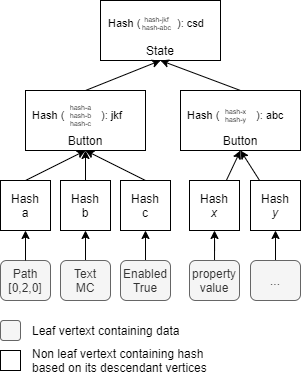
\includegraphics[scale=0.8]{images/merkle-tree-example.png}
\captionof{figure}{An short Merkle tree example based on a widget tree}\label{fig:merkle-tree}
\endgroup

\subsection{How is an inferred model created?}
This research focuses itself on the outcome of the obtain state step as illustrated in figure \ref{fig:obtain-state-graph}, which is the top right part of figure \ref{fig:testar-test-cycle}.

\bigskip
\begingroup
\captionsetup{type=figure}
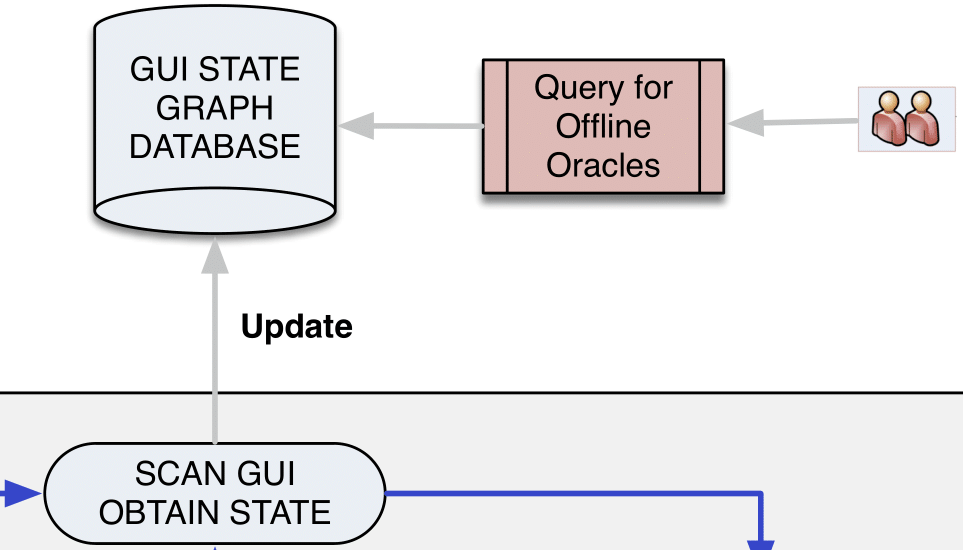
\includegraphics[scale=0.4]{images/obtain-state-graph.png}
\captionof{figure}{The focus of this research proposal \cite{testar-presentation}}\label{fig:obtain-state-graph}
\endgroup

Generating the inferred model starts when \testar start testing the SUT. After an action has been executed successfully, the state of the GUI is sent to the inferred model module. When the state is reached without action, it is marked as the initial state. 

The inferred model module generates the abstract and concrete states and saves those in the model. The model is persisted in the OrientDb database. At last, a deterministic model check is being performed and saved \cite{testar-code}.

\section{State model difference} \label{sec:state-model-difference}
The \verb|StateModel.Difference| package, added by Pastor Ricós\cite{stateDiff}, offers a proof of concept for calculating differences between the inferred state models. For the comparison, the \verb|abstractStateId| is used. 

Pastor Ricós difference algorithm\cite{stateDiff} outputs two classification of changes between two models: added and removed state. Let $A$ be a set of \verb|abstractStateId|s of version 1 of the SUT, and let $B$ be a set of \verb|abstractStateId|s of version 2 of the SUT. The removed states can be written as
\[A-B = \lbrace x | x \in A \wedge x \notin B \rbrace\]
the states that are added can be written as
\[B-A = \lbrace x | x \in B \wedge x \notin A \rbrace\]

\begingroup
\captionsetup{type=figure}
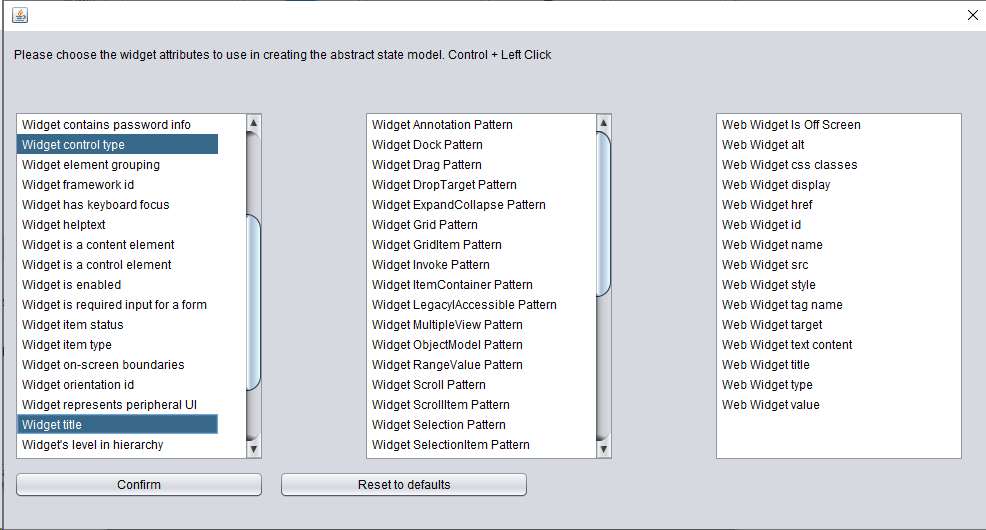
\includegraphics[scale=0.5]{images/attributes-state-model.png}
\captionof{figure}{Select widgets attributes for the abstractStateId}\label{fig:advance}
\endgroup

Using the \verb|abstractStateId| is excellent for the proof of concept and preliminary change detection, 
However, its boolean nature in which state exists or not can result in many 'false' changes. For example, when a widget is moved, the change detection should result in an altered state, not a removed and added state. 

Section \ref{state-identifiers} discussed how identifiers are generated, since the differences are calculated based on the \verb|abstractStateId| selecting the correct widget attributes is vital. Choosing too few attributes could result in conflicting differences like the same actions are removed and added. Choosing too many attributes could trigger a change in even the tiniest detail. Choosing the widget attributes can be done with the 'Advanced' screen under the State model tab. See Figure \ref{fig:advance}.

For the research proposal, an experiment application is created; the two-buttons app. With the two-buttons app, it was possible to experiment with various \testar settings. The application is shown in figures \ref{fig:exp-v1}, \ref{fig:exp-v2} and \ref{fig:exp-v3}. As one can observe, the differences between version 1 and version 2 are the added button with the label 'Hello v2' and between version 2 and 3 the buttons' colour and position. 

\begin{tabularx}{\textwidth}{@{} 
   >{\raggedright\arraybackslash}X
   >{\raggedright\arraybackslash}X  }
    \begingroup
    \captionsetup{type=figure}
    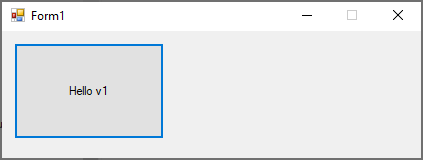
\includegraphics[scale=0.60]{images/exp-v1.png}
    \captionof{figure}{Version 1 of the experiment application}\label{fig:exp-v1}
    \endgroup
    &
    \begingroup
    \captionsetup{type=figure}
    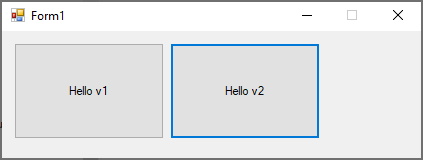
\includegraphics[scale=0.60]{images/exp-v2.png}
    \captionof{figure}{Version 2 of the experiment application}\label{fig:exp-v2}
    \endgroup
    
    \\
    
    \begingroup
    \captionsetup{type=figure}
    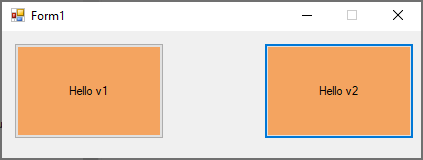
\includegraphics[scale=0.6]{images/exp-v3.png}
    \captionof{figure}{Version 3 of the experiment application}\label{fig:exp-v3}
    \endgroup
\end{tabularx}


However, a different result is displayed when using 'widget title' and 'widget control type' as widget attributes for the abstract states. Namely, the button with the label 'Hello v1' is removed between the first two versions. The buttons labelled 'Hello v1' and 'Hello v2' are added. Between versions 2 and 3, no differences are observed.

This change difference outcome can be explained by the way the proof of concept is working. The widget tree of version 1 contains one button, whereas the widget tree of version 2 contains two buttons. Therefore both the abstract and the concrete identifiers are different for both widget trees. The proof of concept change detection checks whether the abstract identifier of version 1 can be found in version 2, which it cannot, so the state is marked as removed. The state of version 2 can likewise not be found in version 1 so that state is marked as new.

The chosen widget attributes explain the absence of changes between versions 2 and 3. Neither the title nor the control type has changed. Since those attributes were used for the abstract identifier, \testar did not detect a change. 

In section (\ref{research-questions}), the research questions are discussed. Of course, one of the questions will investigate how the change detection algorithm must be implemented. The findings of the two-button app should be considered, and the experiment should be adapted to contain different changes to test on. 

\section{\testar in containers}\label{sec:testar-in-docker}
A recent master thesis by Slomp explains how \testar can be integrated into a \acrfull{ci} environment \cite{thesisSlomp}. Slomp introduced \testar into the world of Docker and container and integrated \testar into an Azure DevOps pipeline. A pipeline is a collection of steps that can automatically build, test and release software. A container bundles all the software, configuration files and libraries together so that an application can run \cite{ms-container}. 

When \testar is being run within the Azure DevOps pipeline, the \testar GUI is not shown. Running \testar is not a problem. However, to analyse the outcome of \testar, the users need to install \testar and have access to the OrientDb database location. 

By moving the code for change detection and visualisation into a stand-alone web application, the user can analyse the outcome on their browser. Since \testar is wrapped into a container, the stand-alone tool will also be wrapped to provide the same infrastructure. Nevertheless, it is up to the IT administrator how they deploy the \testar suite. 

Additionally, to the user's benefit, a \testar developer can also benefit from the application's separation. Changes to either the separate application or \testar can be made without being conflicting with the other. Each tool can focus on one goal, while \testar can focus on testing GUI applications. 
    \newpage
    
    \chapter{Related work}

\todo{make better introduction for related work. }

\subsection{What is a change?} \label{sec:what-is-change}

Not many research papers could be found that define the word change. A clear definition of the word \textit{change} is found in a psychology paper by Rensink \cite{rensink2002change}.

\begin{quote}
    "The word change generally refers to a transformation or modification of something over time. As such, this notion presumes a nonchanging substrate on which changes are imposed. More precisely, change is defined here [the paper] as the transformation over time of a well-defined, enduring structure." (Rensink, 2002, p. 248).
\end{quote}

The definition of the word change can be translated to the language of \testar. The "well-defined, enduring structure" refers to the GUI of the system under test, whereas the "transformation over time" refers to the various version of the SUT. The "something" refers to a part of the GUI that can change like: Widget tree, the state or an action. 

Besides defining the word change, Rensink also describes the differences between changes and differences. A change is a transformation of the same 'something', whether a difference lacks the property of the same something. For example, what are the differences between two distinct SUT, or the same SUT but in two distinct environments or Internet Browsers? A limit to the change detection algorithm is that the SUT needs to be executed in the same environment; otherwise, false-positive changes can occur.

This distinction of definitions between change and differences give the first limit to this research paper's proposed change detection algorithm. The change detection algorithm will give the changes of a SUT, between versions, in the same environment since a different environment can influence the model and therefore influence the outcome of the change detection.

\subsection{What change detection?}


\section{detecting changed by model comp} 

model 

\subsection{Murphy tools}
\todo{After comment resolvement, move Murphy tool from background to this chapter}

GUI driver 

Reference testing GUITAR creates model of current version -> generate test cases... when TC fails -> test failure. 
new features are not failing test cases. 

Browser comparison -> ??

How to compare graphs and visualise them. 

Change visualisation

no much research has been done finding changed in inferred mdoels. There is however a research field that come close to what the research is try to achive, namely cross browser testen. Insted of finding changes between two versions of the same application, with cross browser testing it tries to find differences of the same version but on different browsers.





    \newpage

    \chapter{Research} \label{questions}
In this chapter, the research questions for the thesis are formulated. What research method will be used, and how the questions are being validated.

\section{Context}
The graduation assignment evolves around change detection and visualising the comparison between version of the application under test. The result is an external application that connects to OrientDB and calculates and shows the model comparison. Figure \ref{fig:components-overview} shows the different components involved. The \textit{New Analysis Website} component is the component that is created. Section \ref{sec:components-explained} explained the different components in more detail.

The external application is built as a separate application next to the \testar application. The code that was created by Pastor Ricós (Section \ref{sec:state-model-difference}) and Mulders (Section \ref{inferred-model}) are used as a starting point for the external application. 

\begingroup
\captionsetup{type=figure}
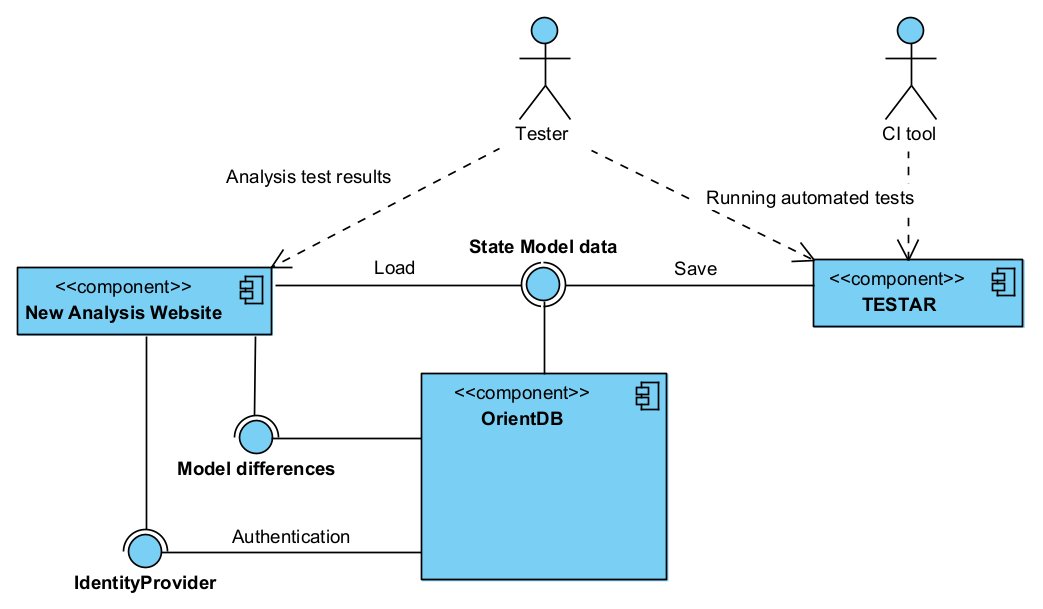
\includegraphics[scale=0.4]{images/3-UML-high-level.png}
\captionof{figure}{Components overview (UML 2.0)}\label{fig:components-overview}
\endgroup

Because change detection is the subject for this graduation assignment, it is assumed that the inferred model generator will generate useful models for change detection. Although the inferred model generator is out-of-scope, it is not ruled out that changes are necessary.

Any automatic learning capabilities are also out-of-scope. A change detection learning capability could be a topic for a future research proposal. Regarding this research proposal, a human will be needed to evaluate the results and outcome of the change detection application.

\section{Research questions} \label{research-questions}
        
The main research question is: \textbf{How can an automated comparison of inferred models help testers finding bugs?}

The main research question is divided into three parts. The first part (\ref{rq:detect-changes}) will research how to detect changes between different versions of the same GUI software (SUT) \cite{testar-todo}. The second part (\ref{rq:diff-visualisation}) will research how to visualise the detected changes. A third Research Question \ref{rq:validation} is dedicated to validating the previous research questions. The research questions are as follows: 


\begin{questions}

    \item How can we set up the change detection as an application written outside of \testar? \label{rq:application-outside-testar}

    \item How to detect changes between two versions of the SUT? \label{rq:detect-changes}
    \begin{questions}
        \item What is change detection, and what do we want to use it for? \label{rq:what-is-change-detection}
        \item Which properties make a model useful for change detection? \label{rq:useful-detection}
        \item Which \testar configuration will generate the useful model? \label{rq:testar-config}
        \item How can we find changes between two models? \label{rq:finding-changes}
    \end{questions}


    
    \item How to visualise the detected differences to the user? \label{rq:diff-visualisation}
    \begin{questions}
        \item What tooling is available to show the result of the change detection? \label{rq:tooling}
        \item How to visualise each change? \label{rq:type-visualisation}
        \item How to generate the shortest set of actions that helps the user to reach the changed state in the SUT? \label{rq:shortest-set}    
    \end{questions}
    
    \item How to validate the results of \ref{rq:detect-changes} and \ref{rq:diff-visualisation}? \label{rq:validation}
    \begin{questions}
        \item What are the requirements for validation applications? \label{rq:req-apps}
        \item Which applications can be used for validation? \label{rq:validation-apps}
    \end{questions}
\end{questions}

\subsection{\ref{rq:application-outside-testar}How can we set up the change detection as an application written outside of \testar?}
\todo{write this section}
extra things had to be done
Industial standards
F-Secure


\subsection{\ref{rq:what-is-change-detection} What is change-detection, and what do we want to use it for?}
To get an answer for \ref{rq:what-is-change-detection}, a literature study will be conducted. The literature study aims to bring an overview of change detection in general and its application in the \testar context. Not only change detection in the GUI but also other change detection methods in the field of Software Engineering, like cross-browser testing. 

\subsection{\ref{rq:useful-detection} Which properties make a model useful for change detection?}
The outcome of \ref{rq:useful-detection} is a list of requirements for the inferred model that are needed to enable change detection. For example, can a non-deterministic state model be used? However, it also includes requirements for the algorithm, like, what are acceptable calculation speeds and how big can a state model be while still complying with the speed requirement? When the set of properties are known, Vaandrager's criteria are used to validate the model \cite{vaandrager}.

\subsection{\ref{rq:testar-config} Which \testar configuration will generate a useful model?}
There are a couple of ways to change the outcome of an inferred model, for example, picking widget attributes for the hash calculation. These configurations can influence the usefulness of the model. The outcome of \ref{rq:useful-detection} should result in a \testar configuration file that configures \testar to generate this useful model. It might be necessary to make code changes in the state model generation or to the identification calculation to implement a Merkle tree approach. Using a Merkle tree could help with comparison to graphs, especially changed in the widget tree. 

A threat of validity for \ref{rq:testar-config} is that every application under test needs its unique configuration. Therefore, it might be wise to look into all widget attributes during the change detection and not take the hash of a state for the comparison. The configuration can be used for tuning the model and the change detection by taking the above approach.

\subsection{\ref{rq:finding-changes} How can we find changes between two models?}
\ref{rq:finding-changes} is the closing question in which the change detection algorithm is coded in Java. In a recent master thesis by Slomp \cite{thesisSlomp}, it is possible to run \testar in a Docker container. As a consequence, \testar can run without a GUI. Therefore the change detection algorithm will run in a separate application, outside the \testar context. The result of the change detection needs to be saved to a data store, preferably the already existing OrientDb database. 

\subsection{\ref{rq:tooling} What tooling is available to show the detected differences?}
Aside from the inferred model, Mulders also created an application to visualise the models. It is essential to state that Mulders did extensive research on which technology fits his needs best. \ref{rq:tooling} will look at the results of Mulders and revalidate whether the libraries are suitable for visualising the differences. 

\subsection{\ref{rq:type-visualisation} How to visualise change?}
\ref{rq:type-visualisation} will look into the execution of the visualisation tool. How can added, removed or altered states in the inferred model be visualised the best? Like \ref{rq:finding-changes} this also includes moving the visualisation tool into its separate application, outside the \testar context. The requirements and GUI proposals will be discussed with the \testar stakeholders. 

\subsection{\ref{rq:shortest-set} How to generate the shortest set of actions that helps the user to reach the changed state in the SUT?}
One of the requirements of the visualisation is showing how to reach the state that has changed. Dijkstra's algorithm \cite{dijkstra1959note} is a well-known algorithm to find the shortest path for a given graph. However, as Goldberg and Harrelson \cite{goldberg2005computing} showed, it is not the most optimal shortest path algorithm, especially with massive graphs. 

\subsection{\ref{rq:req-apps} What are the requirements for validation applications?}
To validate the outcome of the change detection algorithm, we will need to have an application to test it on. The research question will create a set of requirements for the validation application, like multiple versions. The set will be discussed with the supervisors to make sure nothing will be forgotten.

\subsection{\ref{rq:validation-apps} Which applications can be used for validation?}
During development and system testing, the two-button app will be extended and used. Although the app is excellent during the development phase, it is nowhere close to a real-world application. Based on the outcome of \ref{rq:req-apps}, an application needs to be found in order to test the change detection algorithm.

In addition to the application found, F-secure will be asked for feedback on the algorithm and the visualisation. F-Secure is a company based in Finland that provides security solutions to its customers and are currently testing the proof of concept of Pastor Ricós \cite{f-secure}.

With the combination of real-world application and the feedback from F-Secure, biased towards a single point of view for the algorithm will be minimized. 
    \newpage    
    
    \documentclass{ou-report-vaf}

% Dit template is gemaakt door P.J. Molijn in het kader van zijn afstuderen aan de OU in 2014.
% Waarvoor hartelijk dank.
% Minieme maar belangrijke wijzigingen zijn aangebracht door E.M. van Doorn
% Het template is versimpeld door Sylvia Stuurman, 2019.
% Het template is aangepast voor de ba informatica door Harrie Passier, Tanja Vos en Pekka Aho 2020 
% Het tamplate is aangepast met nieuwe huisstyle door Rick Neeft, 2021
% TODO command toegevoegd, 2022

\def\mytitle{How can automated comparison of inferred models help testers finding bugs?}
\def\myauthor{Rick Neeft}
\def\myStudentId{851829973}
\def\myPresentationDate{T.B.D. 2022}

\newcommand{\testar}{\textsc{testar }}
\newcommand{\testarnet}{\textsc{testar .NET }}

\begin{document}

    \pagenumbering{roman}

    % Elements of the thesis
    %%%% TITLE PAGE %%%%%%%
% front cover should be a empty as possible. Title (subtitle) - Name - student Id and thesis presentation date

%to prevent that the title page will be referred as page 1, 
%which will give the warning that there is a page 1 twice.

\pagestyle{plain}

\begin{titlepage}
    \newgeometry{right=100pt,left=58.8pt}

    \pagecolor{ou-light-gray}
    \afterpage{\nopagecolor}
    
    %% Insert the OU logo at the top right corner of the page
    %% PowerPoint contains 84 pt margin in picture
    \begin{tikzpicture}[remember picture,overlay]
                \node at (current page.north east)[anchor=north east,inner sep=58.8pt]{
            
\includegraphics[scale=0.5]{images/ou-text-logo.png}
        };
    \end{tikzpicture}
    
    %% Extra whitespace at the top.
    \vspace*{5\bigskipamount}
    
    %% add title without hypens
    \nohyphens{{\color{ou-red}\Huge\bf \mytitle}}
     
    \bigskip
    %{\large subtitle, if any}
    
    %\bigskip \bigskip
    %by
    \bigskip \bigskip
    
    {\Large\bf \myauthor}\\
    {\large\myStudentId}
    
    {\myPresentationDate}
    
\end{titlepage}

% reset geometry since we changed them for the title page
\newgeometry{right=0.875in,left=.875in}

%%%% END TITLE PAGE %%%%%%%

    % Page 2 must be left blank
    \myemptypage
    
    % Page 3 contains all compulsory data.
    \addcontentsline{toc}{chapter}{Compulsory data}

\myauthor, \myStudentId\\
\textbf{\mytitle}\\
\myPresentationDate
\vspace*{\fill}

Open University of the Netherlands, Faculty of Science\\
Master's Programme in Software Engineering\\
\\
Graduation committee

Chair: Prof. Dr. Tanja E.J. Vos\\
Primary supervisor: Dr. Pekka Aho\\
Seconday supervisor: Fernando Pastor Ricós

Course code: IM9906
\newpage
    
    % Acknowledgements
    \chapter*{Acknowledgements}
\addcontentsline{toc}{chapter}{Acknowledgements}

I want to thank my supervisors, Pekka Aho, Fernando Pastor Ricós and Tanja Vos, for the opportunity and support of my graduation project. The weekly meeting and feedback were always inspiring and gave me good directions on what to do. I am grateful for allowing me to develop the application in C\#. Besides academic learning, using C\# and Blazor is extremely helpful in my day-to-day career.

Thanks to WithSecure, especially Joona Oikarinen and Tatu Aalto, for their input and feedback regarding the Analysis website and the docker setup.

I want to thank my wife for her support and for allowing me to sit in our home office for countless hours. 

Thank you to my family, and special thanks to my mother, who always supported me and pushed me to achieve my life goals. 

Last but not least, I want to thank my employer, VECOZO, for providing me with time and resources to finish my Masters. 

Rick Neeft\\
\myPresentationDate
    %\myemptypage
    
    % Table of contents
    \begingroup
        \hypersetup{linkcolor=black}
        \tableofcontents
    \endgroup
    \newpage
    
    % Summary
    \chapter*{Summary}
\addcontentsline{toc}{chapter}{Summary}
lorem ipsum blah blah yadda yadda yadda
    %\newpage
    
    % the content of the thesis
    \pagenumbering{arabic}
    
    \chapter{Introduction} \label{introduction}
    
Regression testing is considered a good practice when testing new software versions before being released to the general public. 
However, due to shortened release cycles, the time to market has decreased drastically. As a result, software test teams have less time to test all new software features, let alone try all other elements to prevent unwanted side effects \cite{rapid-release-cycle-issues}.
The research proposed aims to apply change detection between two versions of the GUI of the system under test. 

This section introduces the proposed research discussing the background and context, followed by the research problem, research aims, research questions and why this research is important.

\section{Background}
The TESTAR tool solves a significant obstacle when it comes to testing the GUI. With TESTAR, the tester can automatically start testing the GUI without any upfront scripts. TESTAR automatically generates and executes test sequences based on elements derived from the GUI \cite{VosAho2021}. In recent master graduation assignments, TESTAR has been extended with an inferred model generation module \cite{thesisMulders}, and it became easier to integrate TESTAR in build and release pipelines in a DevOps environment \cite{thesisSlomp}. Those two additions make it easier to run TESTAR upon each source code integration and retrieving an inferred model about the GUI. In a proof of concept, two inferred models are compared to get changes between versions of the SUT \cite{stateDiff}.

Some companies might write down changes of the software in a changelog. However, some changelogs might not be complete and unwanted side effects might be missing entirely. Comparing two inferred models shows all the changes between versions of a SUT, even the unwanted ones.

\section{Research problem}
Although the proof of concept for change detection is a good start, it lacks some basic functionality. For example, it compares calculated abstract hashes with each other. As a result, even the slightest change in GUI results in a removed and added state between versions.

In addition to change detection, the change visualisation does not use the build-in visualisation tool. The proof of concept generates an HTML-based report, making it difficult to see where the change can be found and which steps the tester needs to take to navigate to the changed state in the software.

\section{The aim of the research}
The research aims to apply change detection on the inferred model created with the automated GUI testing tool TESTAR and research whether the outcome is helping testers finding bugs quicker. The main research questions are:

\begin{questions}
    \item How to detect changes between two versions of the SUT?
	\item How to visualise the detected differences to the user? 
\item How to validate the results of \ref{rq:detect-changes} and \ref{rq:diff-visualisation}?
\end{questions}

\section{Scope}
The scope of the research is change detection in GUI inferred models created by TESTAR. Researching how to make models and making significant changes to the creation of models are omitted. However, tweaking the model generation, like adding data that is not saved at the moment, and configuring TESTAR to create a good model, are in scope.

\section{Contribution}
When change detection is available in TESTAR, it becomes easy for testers to run the comparison in a continuous integration environment and receive an overview of the changes found in an updated version of the software.

As a side effect, the comparison and visualisation solutions can run outside the context of TESTAR and can be deployed to a docker environment.

\section{Document outline}
This research proposal is structured as follows. In section \ref{intoduction} the context, aim and objectives for this research proposal are introduced, together with the limitations for the expected outcome. Section \ref{background} describes the background of this proposal and contains knowledge that is available but might not be known by the readers. Section \ref{releatedWork} includes an overview of the material that can be seen as a direct foundation for this proposal or work that influences the expected outcome. Section \ref{questions} formulates the research questions for the thesis. The last section \ref{planning} will outline the chosen approach and planning for the graduation assignment.
    \newpage
    
    \chapter{Background} \label{background}

\todo{make better introduction for the chapter. }

This section describes the background of this proposal and contains information that is available but might not be known by students and readers. 

\section{Introduction into GUI Testing}
Ever since the first line of software is written, testers are testing its workings. While in the early day of software, the \acrfull{ui} was mainly terminals based or a set of blinking LEDs \cite{altair8800} \footnote{For example the ALTAIR 8800 computer \cite{altair8800}}, today we have an ever-increasing amount of \acrfull{gui} applications. Testings a GUI application is labour intensive and costs a lot of money \cite{gui-history}.

Initially, testers were using \acrfull{cr} software to automate their work. A tester would record a test scenario into the CR software, and then the CR software will execute the test case when needed. Using CR software, the time required to retest software decreases; however, the big downside is that when software changes, so must the recorded scripts \cite{gui-history}.

Then came \acrfull{mbgt}. With MBGT, the GUI elements and behaviour are abstracted on a higher level. The created models are used to generate abstract test cases. Those abstract test cases need to be mapped or transformed to get concrete test cases that are executed on the SUT. The downside of MBGT is the effort required to create the models and the need to have formal modelling expertise. Formal modelling expertise is not needed with the latest evolution in test automation: model inference. 

The \emph{model inference}, also known as model extraction and GUI Ripping \cite{gui-ripping}, is the current state-of-the-art approach to automate GUI testing \cite{gui-history}. Inferred models are state graphs based on the GUI of the SUT. There are two ways to generate inferred models; the first is a static approach where the source code of the  SUT is used to create a GUI model. The second is a dynamic approach where the GUI state is captured and extracted while being executed. 

The static approach has several downsides. First, the source code must be available, which is not always the case and secondly, it is challenging to capture behaviour based on the GUI source code. For example, with HTML, it is easy to generate a model; however, its behaviour is either in Javascript or server code.  It is possible to overcome those stumbling blocks by executing the SUT.
    
As for the Dynamic approach, it captures the model during test execution. The automated test tool interacts with the SUT in a scriptless and random way. This random scriptless approach is called \emph{Monkey testing}. Usually, test monkeys have no idea in which state the SUT is in and what type of input is allowed. It is therefore essential to make the test monkey smarter. A "smart test monkey" can be achieved by making them "see" the UI elements (Section \ref{data-retrieval}). Section \ref{testar-testauto} will give more details about how \testar is using smart test monkeys.

\section{What is \testar?} \label{what-is-testar}
\testar - or TEST* - is an automated software testing tool for the GUI level \cite{testar-about}. \testar started within the context of the \acrfull{fittest} project. \testar is open-source, the source code is published on GitHub \footnote{ \url{https://github.com/testartool/testar\_dev}}. A screenshot of the \testar tool is displayed in Figure \ref{fig:testar}.

\bigskip
\begingroup
\captionsetup{type=figure}
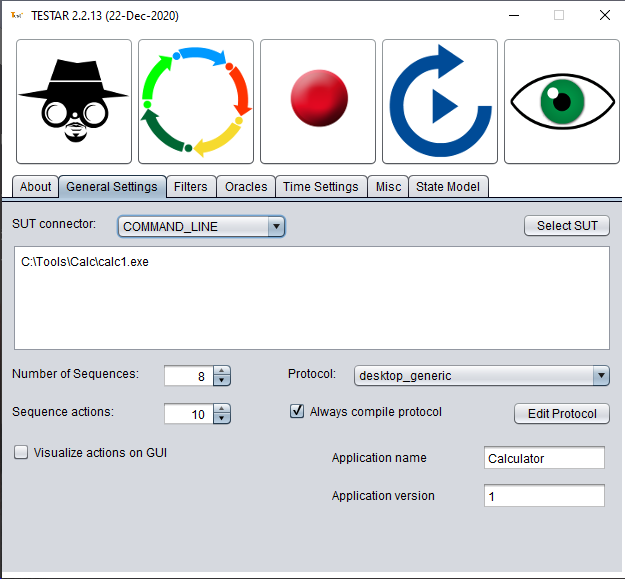
\includegraphics[scale=0.5]{images/testar.png}
\captionof{figure}{Screenshot of the \testar tool}\label{fig:testar}
\endgroup

\testar has several \emph{execution modes} in which it interacts with the SUT \cite{testar-manual}. From left to right, in figure \ref{fig:testar}, those are Spy, Generate, Record, Replay and View mode.

The \emph{Spy} mode allows the user to inspect a SUT and analyse how \testar is interpreting the widgets on the screen. Figure \ref{fig:calc-spy} shows the Windows calculator in spy mode. Dots on the GUI indicate actions that \testar could execute to interact with the SUT. Furthermore, within \testar, it is possible to filter out actions. Then, \testar will not execute those actions. The filtered actions are marked with a grey-coloured dot. A list with properties about the widget is shown when hovering, as well as a unique identifier of the current \emph{state}, more information about the state and the unique identifier can be found at section \ref{gui-state}.\par

\bigskip
\begingroup
\captionsetup{type=figure}
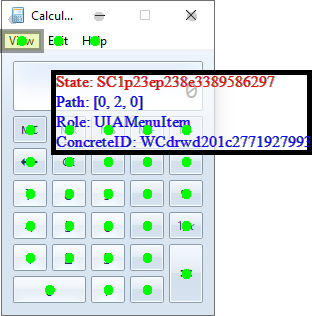
\includegraphics{images/calc-state.png}
\captionof{figure}{Screenshot of the Calculator with \testar Spy}\label{fig:calc-spy}
\endgroup

In the \emph{Generate} mode, \testar will start testing the specified system. Section \ref{testar-testauto} gives more details about \testar test automation.

The \emph{Record} mode allows a tester to record a test sequence manually. In the \emph{Replay} mode, existing test execution can be re-executed and lastly, the \emph{View} mode allows existing test executions to be viewed.

\newpage
\section{TEST automation} \label{testar-testauto}
\testar works without test scripts. Instead, it uses GUI Ripping and Monkey testing techniques. \emph{GUI Ripping}, first introduced by Memon et al. \cite{gui-ripping}, is a process to obtain the GUI's structure and execution behaviour automatically. As for \emph{Monkey testing}, it is a process in which decisions (interactions with the GUI) are randomly made. Section \ref{data-retrieval} will give more insights into GUI Ripping.

\testar is using a flow to execute tests on the SUT. This flow is as follows:
\begin{samepage}
\begin{enumerate}
    \item Start the SUT
    \item Scan the GUI and obtain the state (Section \ref{gui-state})
    \item Finding and selecting an action to execute
    \item Evaluate state with a test oracle (Section \ref{test-oracles})
    \item Stop the SUT when no actions are left to be executed or restart the SUT when more sequences are required.
\end{enumerate}
\end{samepage}

\bigskip
\begingroup
\captionsetup{type=figure}
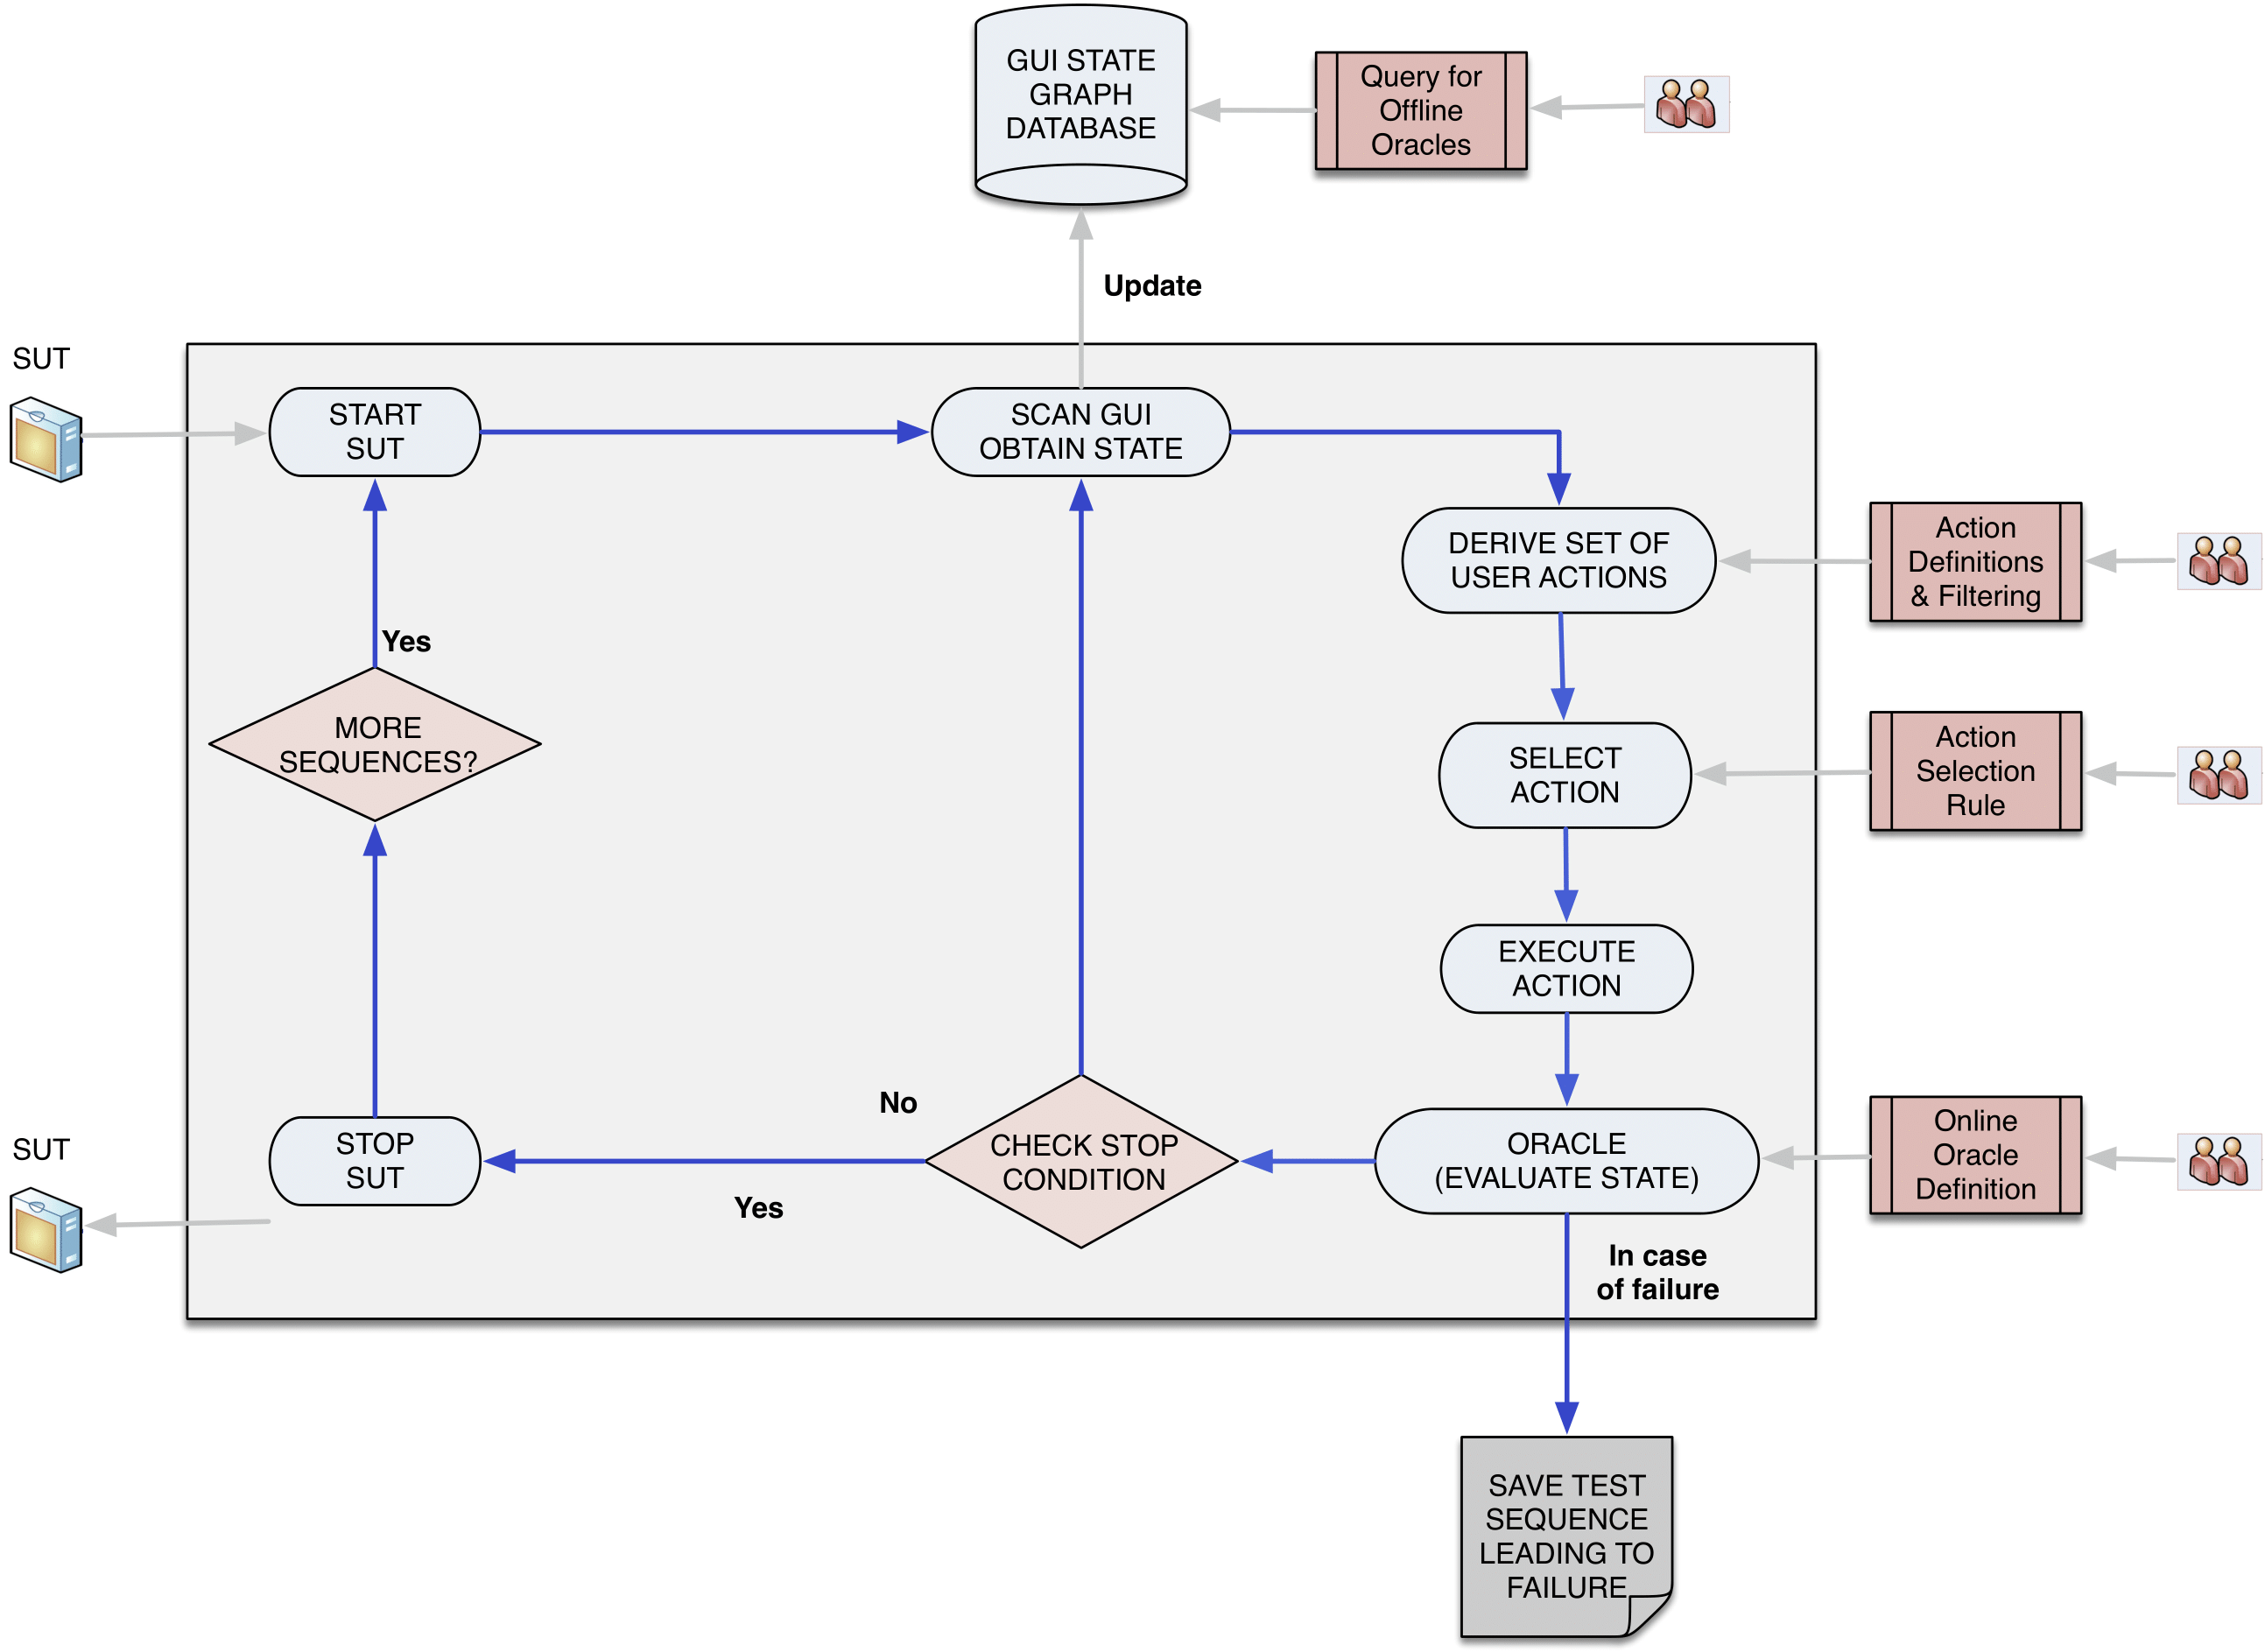
\includegraphics[scale=0.36]{images/testar-test-cycle.png}
\captionof{figure}{\testar test cycle \cite{VosAho2021}}\label{fig:testar-test-cycle}
\endgroup

Figure \ref{fig:testar-test-cycle} shows the flow graphically \cite{VosAho2021}. The test specialist needs to provide SUT details to \testar, like which actions should not be executed, and devise a mechanism that defines which SUT behaviour is correct and which is not, named a test oracle (Section \ref{test-oracles}). 

\section{How is the SUT tested} \label{test-oracles}
When software is tested, a method is needed to check the correct behaviour of the SUT. The method of checking is formally known as a \emph{test oracle} \cite{testOracles}. 

Outside the \testar context, an example of a test oracle could be an \emph{assertion} in software code. An assertion is a boolean expression created in a program by a software developer which checks the program's behaviour during run-time \cite{barr2014oracle}. Assertions can also be used in unit tests as displayed below on Listing \ref{code:assert}. 

\begin{lstlisting}[language=Java, caption=Example assertion, label=code:assert]
@Test
public void testAdd(){
    Calculator sut = new Calculator();

    int expected = 3;
    int actual = sut.Add(1,2);

    Assert.assertEquals(expected, actual);
}
\end{lstlisting}

\testar comes with some test oracles out-of-the-box. Without any configuration, \testar will recognize crashes and unresponsiveness. It is also able to validate the GUI state with suspicious text. For example, a test sequence will fail when the title of a widget contains the word 'exception'. The input for the suspicious text is a regular expression that can be adjusted by the \testar user \cite{VosAho2021}. 

\subsection{Online and Offline Test oracles}
Test oracles come in two variants, \emph{online} or \emph{on-the-fly} test oracles and \emph{offline} test oracles \cite{VosAho2021}. With online test oracles, the state under test is being asserted for any anomalies during test execution. For example,  an online test oracle inspects the URL to check for any information being exposed in the query string. Offline test oracles will look into stored data - like logs - to find anomalies after test execution. For example, offline test oracles can inspect all the visited URLs to check for any exposed information in the query strings.

The two test oracle variants are complementary to each other and can run side by side. However, each variant comes with its strengths and weaknesses. The online test oracle takes up computation time because it inspects the state during test execution. This inspection of state slows down the test execution and may become an issue with time-critical SUTs. On the other hand, some issues - like the SUT becoming unresponsive - can only be checked during test execution. An offline test oracle is inspecting the gathered data after test execution has finished. Especially with larger data sets, this can become helpful. Inspecting the data may run in parallel, which can speed up the test oracle. Additionally, when developers create new offline test oracles, they can inspect the recorded data instead of executing a new test run \cite{de2019offline}.

\section{How is data retrieved} \label{data-retrieval}

Section \ref{testar-testauto} discussed how \testar is using GUI ripping to obtain the GUI's structure. A GUI consists of a non-empty set of UI components, known as \emph{widgets}. Examples of widgets are Windows or buttons; more examples can be found in Table \ref{tables:widgets} \cite{VosAho2021}. 

\begingroup
\captionsetup{type=table}
\begin{tabularx}{\textwidth}{ 
  | >{\raggedright\arraybackslash}X 
  | >{\raggedright\arraybackslash}X 
  | >{\raggedright\arraybackslash}X | }
    \hline
    Windows & Menus & Controls \\
    \hline
    \hline
    main windows & menu bars & buttons \\
    child windows & dropdown menus & textboxes \\
    popup windows & context-aware menus & links \\
    && radio buttons \\
    && checkboxes\\
    && dropdown select boxes\\
    && sliders\\
    && tabs\\
    && scrollbars \\
    \hline
\end{tabularx}
\captionof{table}{Example of GUI widgets \cite{VosAho2021}}\label{tables:widgets}
\endgroup

The widgets are structured hierarchically in a \emph{widget tree}. Each node in the tree is a widget with its related properties, such as the title, position and role. In figure \ref{fig:widget-tree} a compact widget tree is shown for the calculator. 

\bigskip
\begingroup
\captionsetup{type=figure}
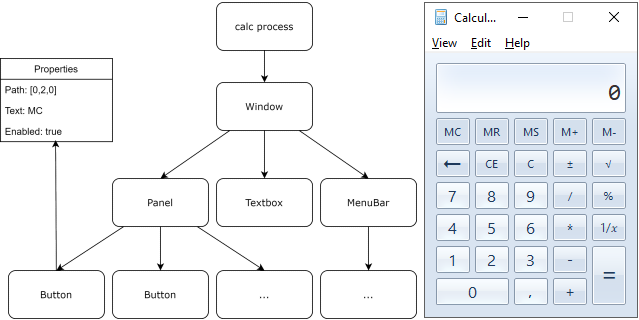
\includegraphics[scale=0.7]{images/calc-tree.png}
\captionof{figure}{A compact version of a widget tree for the calculator.}\label{fig:widget-tree}
\endgroup

\section{Widget data API}

In order to retrieve data from a SUT, \testar is making use of external APIs to access widgets that are part of the GUI \cite{thesisMulders}. \testar is using three different APIs.

In order to test a desktop application, \testar makes use of the Windows Automation API. The purpose of the Windows Automation API is to expose rich information about UI elements\cite{win-api-info}. For web applications, \testar uses Selenium Chromedriver. The Chromedriver is a tool for automated testing. It provides capabilities for navigating through web pages, user input, and JavaScript execution \cite{chrome-driver-info}. The latest API that \testar is using is Appium. Appium is a test automation tool for native, mobile web, and hybrid applications on iOS mobile, Android mobile, and Windows platforms \cite{appium-info}.

\section{GUI State} \label{gui-state}
In the previous sections, the widget tree is discussed and how the widgets are retrieved. In the widget tree, all the GUI elements with their properties are captured. The widget tree represents the state of the GUI when it has stopped executing any action. The GUI is at 'rest'. When an action is executed, the GUI can change, going to a new state. In figure \ref{fig:state-actions} the state change is represented in a small graph. 
\bigskip
\begingroup
\captionsetup{type=figure}
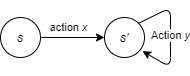
\includegraphics{images/state-action.png}
\captionof{figure}{An graph with two states and two actions.}\label{fig:state-actions}
\endgroup

The graph is a directed graph since every action changes the GUI from one state to the other. An action may lead to the same state, see figure \ref{fig:state-actions} action \textit{y}. However, that would mean that the action does not do anything or \testar does not indicate a change. For example, the GUI changes but the property corresponding to the change is not included in the widget tree.

The universe of states and actions of the SUT's GUI makes up an inferred model. More information about the inferred model and how they are created can be found in section \ref{inferred-model}.

\section{How is data persisted}

\testar is using a database to store and retrieve state model data. Gier and Kager investigated which data storing solution would be beneficial to \testar \cite{GierKager}. The data solution must comply with six requirements. Generally speaking, the requirements were as follows: an open-source graph database with a straightforward query mechanism. The conclusion was that OrientDB was the best solution that met all the requirements.

\begin{samepage}
OrientDB is a Multi-Model NoSQL \acrfull{dbms} that combines four models \cite{orientDbModeling}:

\begin{itemize}
    \item \hyperlink{db:key-value}{Key/Value}
    \item \hyperlink{db:document}{Document}
    \item \hyperlink{db:graph}{Graph}
    \item \hyperlink{db:object}{Object}
\end{itemize}
\end{samepage}

A \hypertarget{db:key-value}{\emph{Key/Value}} is the simplest model and allows storing information (value) that is accessible with a key. Key/Values can be grouped into \textit{buckets}. However, OrientDB supports richer models in the form of document and graph elements.

A \hypertarget{db:document}{\emph{document}} is a schema-less set of key/value pairs. The \emph{key} allows access to the corresponding value. OrientDB allows the developer to store documents into \emph{clusters}. Relations between document are either embedded into other document or \emph{linked} to each other. Someone familiar with relational databases can view a cluster as tables, a document as the row and the key/value pairs are columns.

The \hypertarget{db:graph}{\emph{graph}} is a model consisting of \emph{Vertices} and \emph{Edges}. Vertices are the nodes in the graph, and the edge is the link between those nodes. In \testar terminology, a vertex represents state, and the edge is an 'action' from one state to the next. A Vertex consists of three elements: a unique identifier, a set with incoming Edges and outgoing Edges. An edge consists of four elements: a unique identifier, an incoming vertex (\emph{head}), an outgoing vertex (\emph{tail}) and a label that describes the relationship between the head and tail vertex.\par

The last model is the \hypertarget{db:object}{\emph{object}} that supports inheritance, like in the Object-Oriented programming paradigm.\par

Despite being a NoSQL database, OrientDB does support SQL as a query language \cite{sql-lang} albeit that it does not support all SQL statements. The majority of developers have experience with SQL \cite{sql-stats}, and as a result, new developers and students can start querying the \testar data and start expanding its features.\par

In addition to \testar, other applications can query the state model data in the OrientDB database as well. For example, developers and students can create external tools for a single purpose, like a state model difference application. When building external tools, the \testar application can be kept small and focus upon one objective: testing GUI applications. 

\section{The Murphy tools} \label{murphy-tools}

\todo{This section should go to chapter 3, leaving it here until comment is resolved}

F-Secure, a security software company, based in Finland, developed the Murphy tool \cite{aho2013industrial}. With the Murphy tool, it was possible to automatically extract models from the GUI and use them for GUI testing. The goal of the Murphy tool is to find as many states of a GUI as possible. Users can customise the Murphy scripts to direct the tool to particular cases. 

Like \testar, Murphy creates a directed graph of the GUI under test. Each vertex of the graph is a state of the GUI represented by a screenshot of the GUI. Each edge is an action that the user could perform. 

Like \testar, Murphy is a platform-independent test tool. To accomplish that, Murphy uses various drivers. A driver recognises elements and windows of the GUI under test. One of the drivers uses the 'tab' key to enumerate UI elements. 

While Murphy is crawling the GUI it is making screenshots of the GUI. Besides that, the screenshots represent the state in the graph; they are used to detect changes between different versions of the SUT. 

\section{Inferred model} \label{inferred-model}
The master thesis by Mulders had two significant outcomes. The first is an inferred model module, and the second is the visualisation of the inferred models \cite{thesisMulders}. The visualisation module is a web-based application that shows the inferred model with screenshots and properties. Although the visualisation module will be required when we want to visualise the results of the change-detection software, it is not necessary to go into depth in this document. This section will discuss what an inferred model is and how they are generated. 

The GUI state was discussed in section \ref{gui-state}. The section ended with the sentence that the universe of states and actions of the SUT's GUI makes up the inferred model. The inferred model is a directed graph showing the GUI-state of the application and the transactions between states. The vertex of the graph represents the GUI-state. Each vertex has a set of incoming and outgoing edges, called the actions. 

Figure \ref{fig:state-model} shows the result of the inferred model in the visualisation module.

\bigskip
\begingroup
\captionsetup{type=figure}
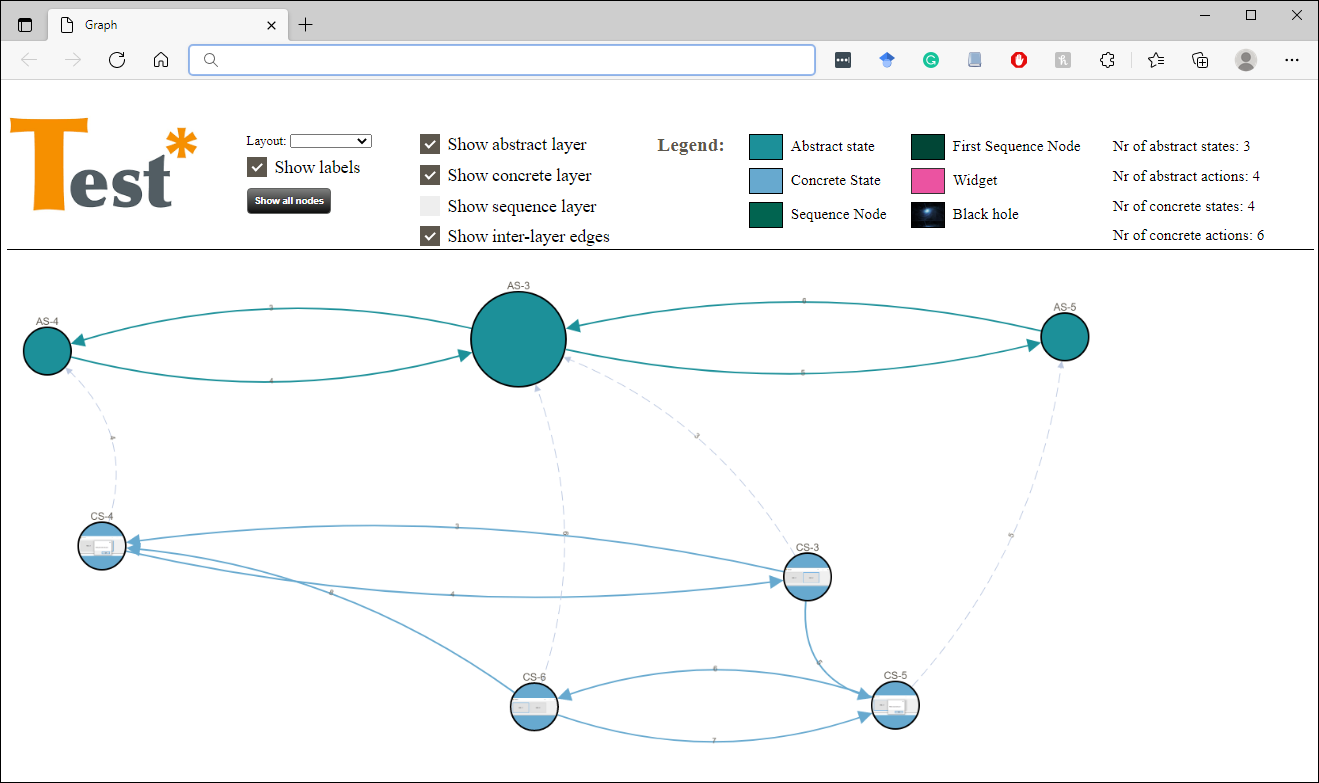
\includegraphics[scale=0.38]{images/state-model.png}
\captionof{figure}{an inferred model in the visualisation application}\label{fig:state-model}
\endgroup

In figure \ref{fig:state-model} two models can be observed. The first model, indicated by the AS text, shows the abstract model. The second, indicated by the CS text, shows the concrete GUI states. 

\subsection{Concrete model}
The concrete model contains all the data that could be retrieved from the GUI. The identification key uses a hash calculated over all the properties. Aside from the widget's properties, the concrete models also contain a screenshot of the GUI for each state \cite{thesisMulders}.

Figure \ref{fig:concrete-node} shows an example of a node in the concrete model. Upon selecting a node, the properties of the node show, including the screenshot taken during the test. The grey dotted line, indicated with the letter 'a', shows the connection with the abstract node, see section \ref{abstract-model} and figure \ref{fig:abstract-model} for more details. The two outgoing edges, indicated with the letter 'b', shows the two actions available in this state. The incoming edge, indicated with the letter 'c', shows how the state was reached. 

\bigskip
\begingroup
\captionsetup{type=figure}
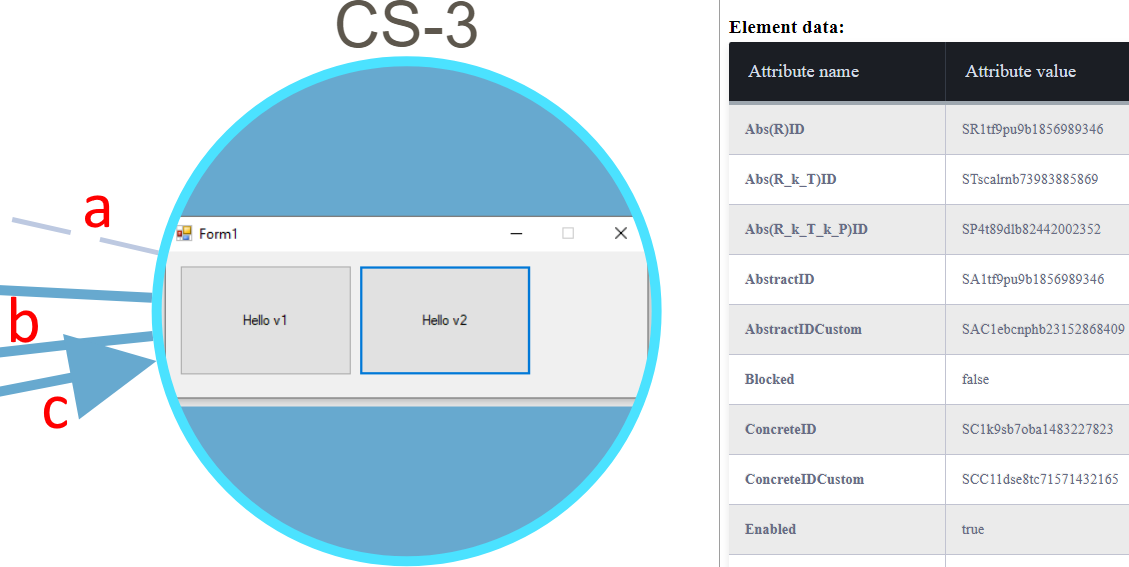
\includegraphics[scale=0.5]{images/concrete-model.png}
\captionof{figure}{A node from the concrete model}\label{fig:concrete-node}
\endgroup

\newpage
\subsection{Abstract model} \label{abstract-model}
Since the concrete models contain all the data from a GUI-state, they can become quite large.  Therefore an abstract state model is made \cite{thesisMulders}. Figure \ref{fig:abstract-model} shows an example of such a abstract node. The grey lines (from CS-3, CS-6 to AS-3) indicates which concrete states are abstracted. The properties of the abstract node are displayed, what the identifier is and which concrete state(s) it represents.

\bigskip
\begingroup
\captionsetup{type=figure}
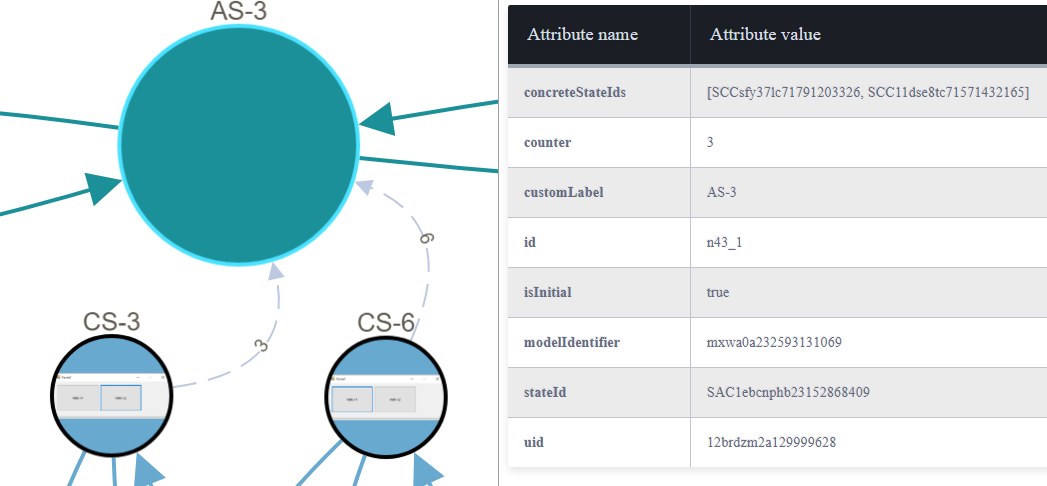
\includegraphics[scale=0.5]{images/abstract-model.png}
\captionof{figure}{A node from the abstract model}\label{fig:abstract-model}
\endgroup

\subsection{State identifiers} \label{state-identifiers}
Every state must have a unique id for identification. The identifier is calculated with the data from the widget tree. 

\testar uses a hashing algorithm that works as follows: the widgets' properties are concatenated and hashed. The outcome will be used as the identifier for a widget. The hashes from the widget in the widget tree are then combined and hashed to create an identifier for the GUI state \cite{VosAho2021}. The \testar's algorithm is similar to how a Merkle tree works, more information can be found at section \ref{merkle-tree}.

To identify the state (and actions), \testar calculates two state identifiers; an abstract and concrete state identifier. For the concrete state identifier, all the properties of a widget are used. For the abstract identifier, a subset of the properties is used. It is configurable which properties are used for the abstract identifier. By default the properties \textit{role}, \textit{title}, \textit{position} and \textit{enabled} are utilised \cite{VosAho2021, thesisMulders}.

When running \testar, it is possible to configure which widget properties should be used for the abstract state identifier. Figure \ref{fig:advance} shows the selection dialogue in which the user can select the properties for the abstract identifier.

\section{Merkle tree} \label{merkle-tree}
A Merkle tree is a hash tree data structure where a hash can identify each vertex. \cite{merkle-tree} The cryptographic hash is calculated by taking the hashes of the descendant vertices, combining them, and calculating a new hash from the combination. 

As written in the previous section (\ref{state-identifiers}), \testar's way of calculating the identification id for a widget or a GUI state is similar to that of the Merkle tree vertex. The hashed id for a widget is based on the hashed property values. Figure \ref{fig:merkle-tree} shows an example of a Merkle tree about how the GUI state identification id is calculated. The corresponding widget tree (Figure \ref{fig:widget-tree}), where the Merkle tree is based, is shown in the top right corner.

Although a Merkle tree usually is a binary tree \cite{merkle-tree}, having more than two descendant vertices is not considered a problem since the same Merkle-tree principle can be applied.

\bigskip
\begingroup
\captionsetup{type=figure}
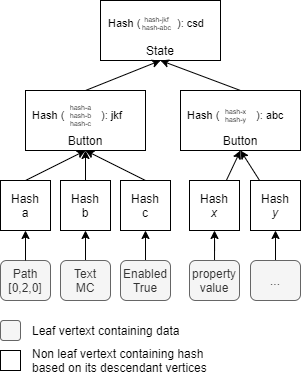
\includegraphics[scale=0.8]{images/merkle-tree-example.png}
\captionof{figure}{An short Merkle tree example based on a widget tree}\label{fig:merkle-tree}
\endgroup

\subsection{How is an inferred model created?}
This research focuses itself on the outcome of the obtain state step as illustrated in figure \ref{fig:obtain-state-graph}, which is the top right part of figure \ref{fig:testar-test-cycle}.

\bigskip
\begingroup
\captionsetup{type=figure}
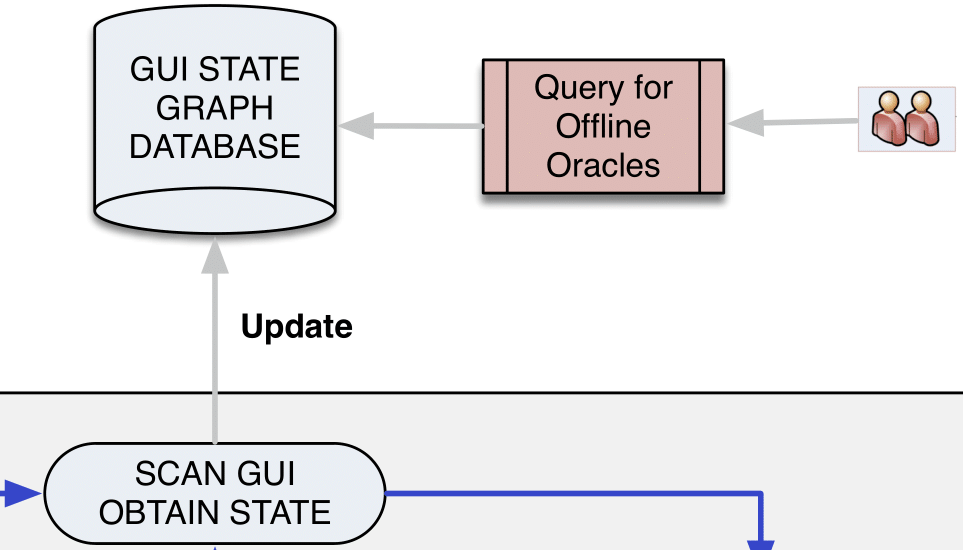
\includegraphics[scale=0.4]{images/obtain-state-graph.png}
\captionof{figure}{The focus of this research proposal \cite{testar-presentation}}\label{fig:obtain-state-graph}
\endgroup

Generating the inferred model starts when \testar start testing the SUT. After an action has been executed successfully, the state of the GUI is sent to the inferred model module. When the state is reached without action, it is marked as the initial state. 

The inferred model module generates the abstract and concrete states and saves those in the model. The model is persisted in the OrientDb database. At last, a deterministic model check is being performed and saved \cite{testar-code}.

\section{State model difference} \label{sec:state-model-difference}
The \verb|StateModel.Difference| package, added by Pastor Ricós\cite{stateDiff}, offers a proof of concept for calculating differences between the inferred state models. For the comparison, the \verb|abstractStateId| is used. 

Pastor Ricós difference algorithm\cite{stateDiff} outputs two classification of changes between two models: added and removed state. Let $A$ be a set of \verb|abstractStateId|s of version 1 of the SUT, and let $B$ be a set of \verb|abstractStateId|s of version 2 of the SUT. The removed states can be written as
\[A-B = \lbrace x | x \in A \wedge x \notin B \rbrace\]
the states that are added can be written as
\[B-A = \lbrace x | x \in B \wedge x \notin A \rbrace\]

\begingroup
\captionsetup{type=figure}
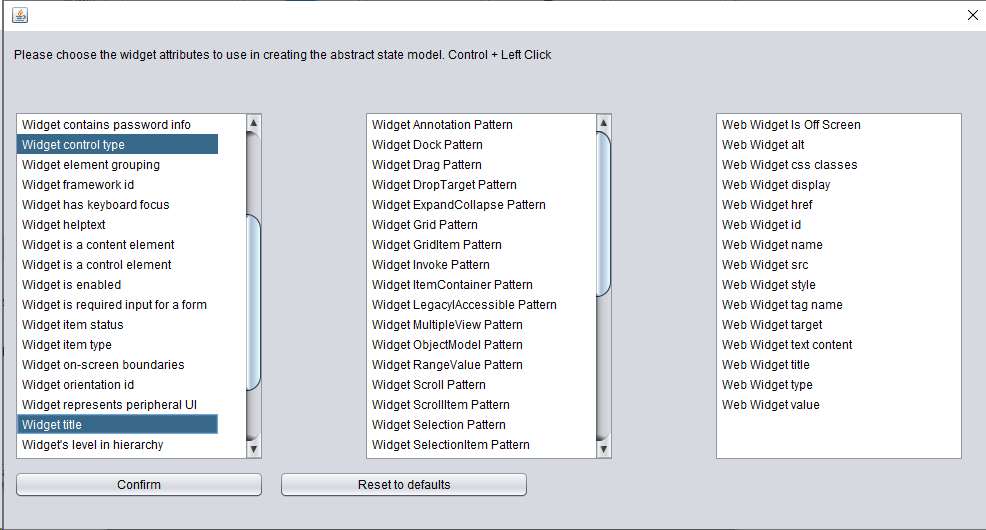
\includegraphics[scale=0.5]{images/attributes-state-model.png}
\captionof{figure}{Select widgets attributes for the abstractStateId}\label{fig:advance}
\endgroup

Using the \verb|abstractStateId| is excellent for the proof of concept and preliminary change detection, 
However, its boolean nature in which state exists or not can result in many 'false' changes. For example, when a widget is moved, the change detection should result in an altered state, not a removed and added state. 

Section \ref{state-identifiers} discussed how identifiers are generated, since the differences are calculated based on the \verb|abstractStateId| selecting the correct widget attributes is vital. Choosing too few attributes could result in conflicting differences like the same actions are removed and added. Choosing too many attributes could trigger a change in even the tiniest detail. Choosing the widget attributes can be done with the 'Advanced' screen under the State model tab. See Figure \ref{fig:advance}.

For the research proposal, an experiment application is created; the two-buttons app. With the two-buttons app, it was possible to experiment with various \testar settings. The application is shown in figures \ref{fig:exp-v1}, \ref{fig:exp-v2} and \ref{fig:exp-v3}. As one can observe, the differences between version 1 and version 2 are the added button with the label 'Hello v2' and between version 2 and 3 the buttons' colour and position. 

\begin{tabularx}{\textwidth}{@{} 
   >{\raggedright\arraybackslash}X
   >{\raggedright\arraybackslash}X  }
    \begingroup
    \captionsetup{type=figure}
    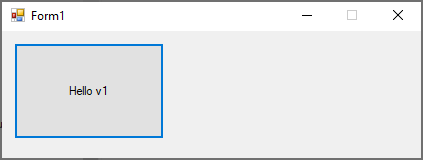
\includegraphics[scale=0.60]{images/exp-v1.png}
    \captionof{figure}{Version 1 of the experiment application}\label{fig:exp-v1}
    \endgroup
    &
    \begingroup
    \captionsetup{type=figure}
    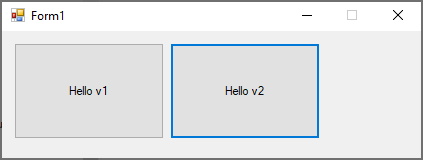
\includegraphics[scale=0.60]{images/exp-v2.png}
    \captionof{figure}{Version 2 of the experiment application}\label{fig:exp-v2}
    \endgroup
    
    \\
    
    \begingroup
    \captionsetup{type=figure}
    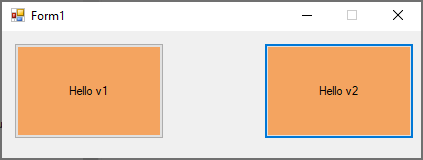
\includegraphics[scale=0.6]{images/exp-v3.png}
    \captionof{figure}{Version 3 of the experiment application}\label{fig:exp-v3}
    \endgroup
\end{tabularx}


However, a different result is displayed when using 'widget title' and 'widget control type' as widget attributes for the abstract states. Namely, the button with the label 'Hello v1' is removed between the first two versions. The buttons labelled 'Hello v1' and 'Hello v2' are added. Between versions 2 and 3, no differences are observed.

This change difference outcome can be explained by the way the proof of concept is working. The widget tree of version 1 contains one button, whereas the widget tree of version 2 contains two buttons. Therefore both the abstract and the concrete identifiers are different for both widget trees. The proof of concept change detection checks whether the abstract identifier of version 1 can be found in version 2, which it cannot, so the state is marked as removed. The state of version 2 can likewise not be found in version 1 so that state is marked as new.

The chosen widget attributes explain the absence of changes between versions 2 and 3. Neither the title nor the control type has changed. Since those attributes were used for the abstract identifier, \testar did not detect a change. 

In section (\ref{research-questions}), the research questions are discussed. Of course, one of the questions will investigate how the change detection algorithm must be implemented. The findings of the two-button app should be considered, and the experiment should be adapted to contain different changes to test on. 

\section{\testar in containers}\label{sec:testar-in-docker}
A recent master thesis by Slomp explains how \testar can be integrated into a \acrfull{ci} environment \cite{thesisSlomp}. Slomp introduced \testar into the world of Docker and container and integrated \testar into an Azure DevOps pipeline. A pipeline is a collection of steps that can automatically build, test and release software. A container bundles all the software, configuration files and libraries together so that an application can run \cite{ms-container}. 

When \testar is being run within the Azure DevOps pipeline, the \testar GUI is not shown. Running \testar is not a problem. However, to analyse the outcome of \testar, the users need to install \testar and have access to the OrientDb database location. 

By moving the code for change detection and visualisation into a stand-alone web application, the user can analyse the outcome on their browser. Since \testar is wrapped into a container, the stand-alone tool will also be wrapped to provide the same infrastructure. Nevertheless, it is up to the IT administrator how they deploy the \testar suite. 

Additionally, to the user's benefit, a \testar developer can also benefit from the application's separation. Changes to either the separate application or \testar can be made without being conflicting with the other. Each tool can focus on one goal, while \testar can focus on testing GUI applications. 
    \newpage
    
    \chapter{Related work}

\todo{make better introduction for related work. }

\subsection{What is a change?} \label{sec:what-is-change}

Not many research papers could be found that define the word change. A clear definition of the word \textit{change} is found in a psychology paper by Rensink \cite{rensink2002change}.

\begin{quote}
    "The word change generally refers to a transformation or modification of something over time. As such, this notion presumes a nonchanging substrate on which changes are imposed. More precisely, change is defined here [the paper] as the transformation over time of a well-defined, enduring structure." (Rensink, 2002, p. 248).
\end{quote}

The definition of the word change can be translated to the language of \testar. The "well-defined, enduring structure" refers to the GUI of the system under test, whereas the "transformation over time" refers to the various version of the SUT. The "something" refers to a part of the GUI that can change like: Widget tree, the state or an action. 

Besides defining the word change, Rensink also describes the differences between changes and differences. A change is a transformation of the same 'something', whether a difference lacks the property of the same something. For example, what are the differences between two distinct SUT, or the same SUT but in two distinct environments or Internet Browsers? A limit to the change detection algorithm is that the SUT needs to be executed in the same environment; otherwise, false-positive changes can occur.

This distinction of definitions between change and differences give the first limit to this research paper's proposed change detection algorithm. The change detection algorithm will give the changes of a SUT, between versions, in the same environment since a different environment can influence the model and therefore influence the outcome of the change detection.

\subsection{What change detection?}


\section{detecting changed by model comp} 

model 

\subsection{Murphy tools}
\todo{After comment resolvement, move Murphy tool from background to this chapter}

GUI driver 

Reference testing GUITAR creates model of current version -> generate test cases... when TC fails -> test failure. 
new features are not failing test cases. 

Browser comparison -> ??

How to compare graphs and visualise them. 

Change visualisation

no much research has been done finding changed in inferred mdoels. There is however a research field that come close to what the research is try to achive, namely cross browser testen. Insted of finding changes between two versions of the same application, with cross browser testing it tries to find differences of the same version but on different browsers.





    \newpage

    \chapter{Research} \label{questions}
In this chapter, the research questions for the thesis are formulated. What research method will be used, and how the questions are being validated.

\section{Context}
The graduation assignment evolves around change detection and visualising the comparison between version of the application under test. The result is an external application that connects to OrientDB and calculates and shows the model comparison. Figure \ref{fig:components-overview} shows the different components involved. The \textit{New Analysis Website} component is the component that is created. Section \ref{sec:components-explained} explained the different components in more detail.

The external application is built as a separate application next to the \testar application. The code that was created by Pastor Ricós (Section \ref{sec:state-model-difference}) and Mulders (Section \ref{inferred-model}) are used as a starting point for the external application. 

\begingroup
\captionsetup{type=figure}
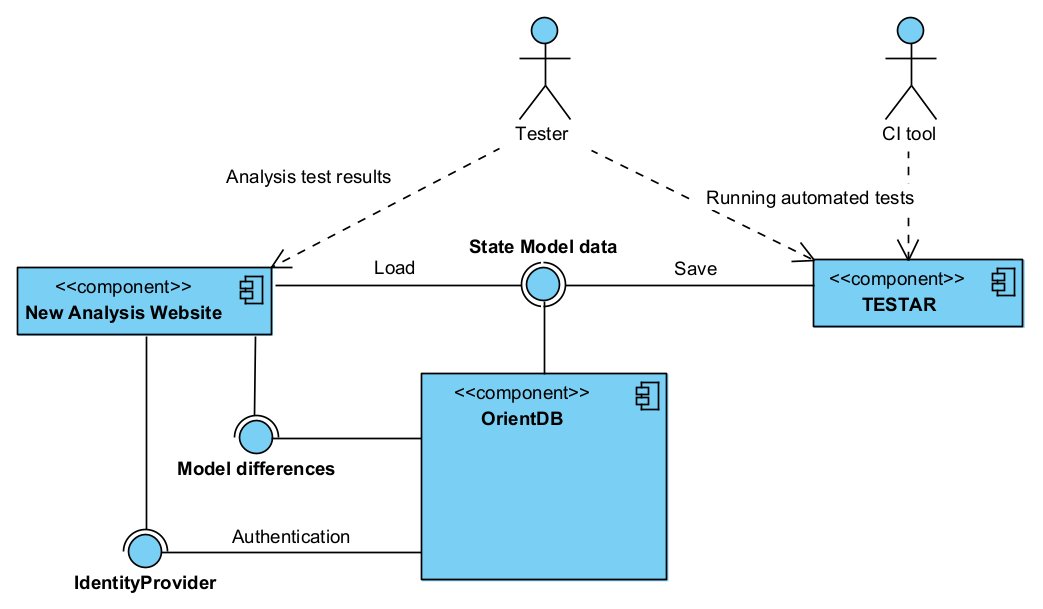
\includegraphics[scale=0.4]{images/3-UML-high-level.png}
\captionof{figure}{Components overview (UML 2.0)}\label{fig:components-overview}
\endgroup

Because change detection is the subject for this graduation assignment, it is assumed that the inferred model generator will generate useful models for change detection. Although the inferred model generator is out-of-scope, it is not ruled out that changes are necessary.

Any automatic learning capabilities are also out-of-scope. A change detection learning capability could be a topic for a future research proposal. Regarding this research proposal, a human will be needed to evaluate the results and outcome of the change detection application.

\section{Research questions} \label{research-questions}
        
The main research question is: \textbf{How can an automated comparison of inferred models help testers finding bugs?}

The main research question is divided into three parts. The first part (\ref{rq:detect-changes}) will research how to detect changes between different versions of the same GUI software (SUT) \cite{testar-todo}. The second part (\ref{rq:diff-visualisation}) will research how to visualise the detected changes. A third Research Question \ref{rq:validation} is dedicated to validating the previous research questions. The research questions are as follows: 


\begin{questions}

    \item How can we set up the change detection as an application written outside of \testar? \label{rq:application-outside-testar}

    \item How to detect changes between two versions of the SUT? \label{rq:detect-changes}
    \begin{questions}
        \item What is change detection, and what do we want to use it for? \label{rq:what-is-change-detection}
        \item Which properties make a model useful for change detection? \label{rq:useful-detection}
        \item Which \testar configuration will generate the useful model? \label{rq:testar-config}
        \item How can we find changes between two models? \label{rq:finding-changes}
    \end{questions}


    
    \item How to visualise the detected differences to the user? \label{rq:diff-visualisation}
    \begin{questions}
        \item What tooling is available to show the result of the change detection? \label{rq:tooling}
        \item How to visualise each change? \label{rq:type-visualisation}
        \item How to generate the shortest set of actions that helps the user to reach the changed state in the SUT? \label{rq:shortest-set}    
    \end{questions}
    
    \item How to validate the results of \ref{rq:detect-changes} and \ref{rq:diff-visualisation}? \label{rq:validation}
    \begin{questions}
        \item What are the requirements for validation applications? \label{rq:req-apps}
        \item Which applications can be used for validation? \label{rq:validation-apps}
    \end{questions}
\end{questions}

\subsection{\ref{rq:application-outside-testar}How can we set up the change detection as an application written outside of \testar?}
\todo{write this section}
extra things had to be done
Industial standards
F-Secure


\subsection{\ref{rq:what-is-change-detection} What is change-detection, and what do we want to use it for?}
To get an answer for \ref{rq:what-is-change-detection}, a literature study will be conducted. The literature study aims to bring an overview of change detection in general and its application in the \testar context. Not only change detection in the GUI but also other change detection methods in the field of Software Engineering, like cross-browser testing. 

\subsection{\ref{rq:useful-detection} Which properties make a model useful for change detection?}
The outcome of \ref{rq:useful-detection} is a list of requirements for the inferred model that are needed to enable change detection. For example, can a non-deterministic state model be used? However, it also includes requirements for the algorithm, like, what are acceptable calculation speeds and how big can a state model be while still complying with the speed requirement? When the set of properties are known, Vaandrager's criteria are used to validate the model \cite{vaandrager}.

\subsection{\ref{rq:testar-config} Which \testar configuration will generate a useful model?}
There are a couple of ways to change the outcome of an inferred model, for example, picking widget attributes for the hash calculation. These configurations can influence the usefulness of the model. The outcome of \ref{rq:useful-detection} should result in a \testar configuration file that configures \testar to generate this useful model. It might be necessary to make code changes in the state model generation or to the identification calculation to implement a Merkle tree approach. Using a Merkle tree could help with comparison to graphs, especially changed in the widget tree. 

A threat of validity for \ref{rq:testar-config} is that every application under test needs its unique configuration. Therefore, it might be wise to look into all widget attributes during the change detection and not take the hash of a state for the comparison. The configuration can be used for tuning the model and the change detection by taking the above approach.

\subsection{\ref{rq:finding-changes} How can we find changes between two models?}
\ref{rq:finding-changes} is the closing question in which the change detection algorithm is coded in Java. In a recent master thesis by Slomp \cite{thesisSlomp}, it is possible to run \testar in a Docker container. As a consequence, \testar can run without a GUI. Therefore the change detection algorithm will run in a separate application, outside the \testar context. The result of the change detection needs to be saved to a data store, preferably the already existing OrientDb database. 

\subsection{\ref{rq:tooling} What tooling is available to show the detected differences?}
Aside from the inferred model, Mulders also created an application to visualise the models. It is essential to state that Mulders did extensive research on which technology fits his needs best. \ref{rq:tooling} will look at the results of Mulders and revalidate whether the libraries are suitable for visualising the differences. 

\subsection{\ref{rq:type-visualisation} How to visualise change?}
\ref{rq:type-visualisation} will look into the execution of the visualisation tool. How can added, removed or altered states in the inferred model be visualised the best? Like \ref{rq:finding-changes} this also includes moving the visualisation tool into its separate application, outside the \testar context. The requirements and GUI proposals will be discussed with the \testar stakeholders. 

\subsection{\ref{rq:shortest-set} How to generate the shortest set of actions that helps the user to reach the changed state in the SUT?}
One of the requirements of the visualisation is showing how to reach the state that has changed. Dijkstra's algorithm \cite{dijkstra1959note} is a well-known algorithm to find the shortest path for a given graph. However, as Goldberg and Harrelson \cite{goldberg2005computing} showed, it is not the most optimal shortest path algorithm, especially with massive graphs. 

\subsection{\ref{rq:req-apps} What are the requirements for validation applications?}
To validate the outcome of the change detection algorithm, we will need to have an application to test it on. The research question will create a set of requirements for the validation application, like multiple versions. The set will be discussed with the supervisors to make sure nothing will be forgotten.

\subsection{\ref{rq:validation-apps} Which applications can be used for validation?}
During development and system testing, the two-button app will be extended and used. Although the app is excellent during the development phase, it is nowhere close to a real-world application. Based on the outcome of \ref{rq:req-apps}, an application needs to be found in order to test the change detection algorithm.

In addition to the application found, F-secure will be asked for feedback on the algorithm and the visualisation. F-Secure is a company based in Finland that provides security solutions to its customers and are currently testing the proof of concept of Pastor Ricós \cite{f-secure}.

With the combination of real-world application and the feedback from F-Secure, biased towards a single point of view for the algorithm will be minimized. 
    \newpage    
    
    \documentclass{ou-report-vaf}

% Dit template is gemaakt door P.J. Molijn in het kader van zijn afstuderen aan de OU in 2014.
% Waarvoor hartelijk dank.
% Minieme maar belangrijke wijzigingen zijn aangebracht door E.M. van Doorn
% Het template is versimpeld door Sylvia Stuurman, 2019.
% Het template is aangepast voor de ba informatica door Harrie Passier, Tanja Vos en Pekka Aho 2020 
% Het tamplate is aangepast met nieuwe huisstyle door Rick Neeft, 2021
% TODO command toegevoegd, 2022

\def\mytitle{How can automated comparison of inferred models help testers finding bugs?}
\def\myauthor{Rick Neeft}
\def\myStudentId{851829973}
\def\myPresentationDate{T.B.D. 2022}

\newcommand{\testar}{\textsc{testar }}
\newcommand{\testarnet}{\textsc{testar .NET }}

\begin{document}

    \pagenumbering{roman}

    % Elements of the thesis
    \input{front-cover}

    % Page 2 must be left blank
    \myemptypage
    
    % Page 3 contains all compulsory data.
    \input{compulsory-data}
    
    % Acknowledgements
    \input{content/A-Acknowledgements}
    %\myemptypage
    
    % Table of contents
    \begingroup
        \hypersetup{linkcolor=black}
        \tableofcontents
    \endgroup
    \newpage
    
    % Summary
    \input{content/B-Summary}
    %\newpage
    
    % the content of the thesis
    \pagenumbering{arabic}
    
    \input{content/1-Introduction}
    \newpage
    
    \input{content/2-Background}
    \newpage
    
    \input{content/3-Related-Work}
    \newpage

    \input{content/4-Research}
    \newpage    
    
    \input{content/5-Results/main}
    \newpage
    
    \input{content/6-Experiments}
    \newpage
    
    % Reference list
    \bibliographystyle{abbrv}
    \bibliography{bibliography}
    \newpage
    
    % List of abbreviations
    
    
    % Appendices
    \appendix
    \input{content/Appendixes/main}


\end{document}
    \newpage
    
    \chapter{Validation \& Experiments} \label{chapter:validation-experiments}

In this chapter, the validation of the algorithm is tested. This testing happens in three tests. Section \ref{sec:scenarios-testing} presents the findings of a technical test in which test scenarios are designed to test the algorithm. It starts with setting up in-memory graphs and asserting the outcome of the merge graph. Section \ref{sec:experimental-application} shows the use of an external application tested by \testar. The external application is an experimental test application in which it is possible to create three different versions.

\todo{The last test is conducted using a real-life application, tested by \testar. }

\section{Technical testing} \label{sec:scenarios-testing}
The first form of algorithm validation is a technical test done with Gherkin syntax. \textit{Gherkin} is a syntax that describes a test scenario. The syntax uses special keywords like \textbf{Given}, \textbf{When}, \textbf{Then} to describe a \textit{scenario}. An example of a Gherkin scenario can be found in listing \ref{code:gherkin-example}.

\begin{lstlisting}[language=Gherkin, caption=Calculator test example, label=code:gherkin-example]
Scenario: Add two numbers
Given the first number is 50
And the second number is 70
When the two numbers are added
Then the result should be 120
\end{lstlisting}

A developer can automate the Gherkin syntax to create automated test cases with, for example, the help of Specflow \footnote{\url{https://www.specflow.com}}. Specflow is a test automation solution for the .NET framework \cite{specflow}. The code to automate the 'then' line in listing \ref{code:gherkin-example} can be implemented as indicated in listing \ref{code:gherkin-example-code}.

\begin{lstlisting}[language=Java, caption=Implementation of a 'then' line, label=code:gherkin-example-code]
[Then("the result should be (.*)")]
public void ThenTheResultShouldBe(int expectedResult)
{
    Assert.AreEqual(expectedResult, actualResult);
}
\end{lstlisting}

A couple of scenarios are written to validate the algorithm and the merging of the two abstract models (see \ref{sec:merge-graph}). The scenario's can be found in appendix \ref{appendix:test-scenarios}. The file starts with the keyword \textbf{Feature} which is a Specflow solution to group scenarios together. The \textbf{Background} section generates four in-memory graphs. Figure \ref{fig:test-graphs} visualises the four graphs. 

\begingroup
\captionsetup{type=figure}
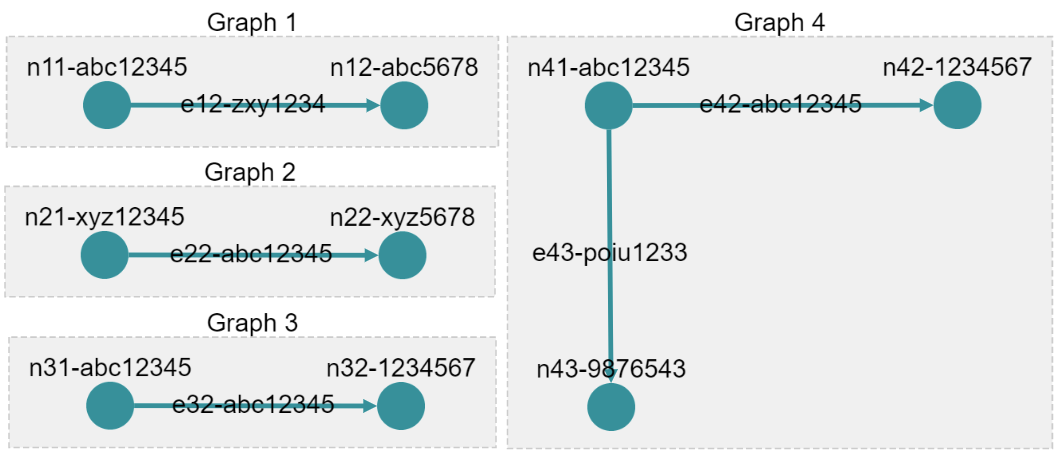
\includegraphics[scale=0.6]{images/6-TestGraphs.png}
\captionof{figure}{Test graphs used for testing. The circle represents an abstract state, and the line represents the abstract actions between the abstract states}\label{fig:test-graphs}
\endgroup

Each scenario follows the same pattern. The first two graphs from the background are chosen and set as either the old or new. Then the comparison is run, and the comparison result is merged. After the merge, the actual result is asserted with the validation described. Five scenarios are tested using this pattern, divided into four specific tests focusing on a specific qualification of a change. The fifth scenario is a more extensive test representing the experiment application discussed in the next section.

The four specific tests are as follows (1) validation that the initial states are recognised as corresponding states, (2) Going from a corresponding state, following action with the same id, validating that the target state is recognised as corresponding states, (3) When a new abstract state is added validate it is recognised and merge as such, (4) When an abstract state is removed in the new version validate it is recognised and merged as such.

The fifth scenario used two different graphs, which are visualised in figure \ref{fig:bigger-test-graphs}. The graphs both have the same initial state, going to an intermediate state where actions v1, v2 and v3 can be executed. In graph six, the v3 action has been added, and the v1 action is removed. A merge graph is generated by running the scenario, which is visualised in figure \ref{fig:test-merged-graph}. The merge graph is what was expected. 

\begingroup
\captionsetup{type=figure}
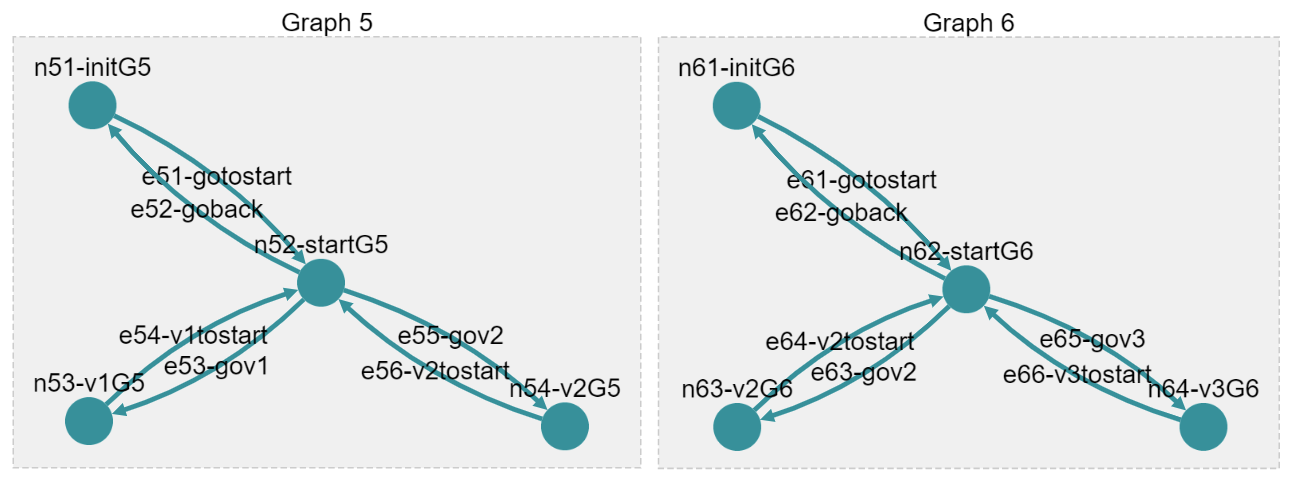
\includegraphics[scale=0.5]{images/6-test-graph-5-6.png}
\captionof{figure}{Graphs 5 and 6 for the bigger scenario. The circle represents an abstract state. The line represents the abstract actions between the abstract states}\label{fig:bigger-test-graphs}
\endgroup

The merge graph uses different colours and shapes to indicate removed and added states. Using an alternative form of representing the outcome, besides colours, makes it possible to distinguish normal, removed or added states even when the results are printed in black-and-white or with people who are colour blind. A red triangle represents a removed abstract state. A green star indicates a new abstract state.

\begingroup
\captionsetup{type=figure}
\includegraphics[scale=0.5]{images/6-merge-result.png}
\captionof{figure}{The merge result is visualised. The circle represents an abstract state, a green star represents a new and, the red triangle represents a removed abstract state, and the line represents the abstract actions between the abstract states }\label{fig:test-merged-graph}
\endgroup


\subsection{Outcome of the technical tests}
By running the scenario, one issue was found in the merge engine. Section \ref{sec:merge-graph} explains that the edged (abstract actions in \testar case) must be rewired from the old graph to the merge graph. Adding all the old edges led to duplication of actions since corresponding actions were already present in the merge graph. The issue was fixed by keeping track of the action id while making the merge graph. When an action already existed in the set of action Id, the action was skipped for rewiring. 

\section{Experimental application} \label{sec:experimental-application}

\subsection{The application}

The application under test is an application created in .NET. The source code can be found in the companion GitHub repository \footnote{\url{https://github.com/rneeft/study-ga/tree/main/experiment/TestarChangeDetectionExperiment}}. The application is an upgraded two-button application mentioned in section \ref{sec:state-model-difference}. Figure \ref{fig:experiment-start} shows the start screen of the experiment application whereas figures \ref{fig:experiment-v1}, \ref{fig:experiment-v2} and \ref{fig:experiment-v2}  shows the three different versions. The start screen is added, and the back button enables going back to ensure the initial state of all the applications is equal. 

\begin{tabularx}{\textwidth}{@{} 
   >{\raggedright\arraybackslash}X
   >{\raggedright\arraybackslash}X  }
    \begingroup
    \captionsetup{type=figure}
    \includegraphics[scale=0.60]{images/6-Experiment-Start.png}
    \captionof{figure}{Start screen}\label{fig:experiment-start}
    \endgroup
    &
    \begingroup
    \captionsetup{type=figure}
    \includegraphics[scale=0.60]{images/6-Experiment-v1.png}
    \captionof{figure}{Version 1}\label{fig:experiment-v1}
    \endgroup
    
    \\
    
    \begingroup
    \captionsetup{type=figure}
    \includegraphics[scale=0.6]{images/6-Experiment-v2.png}
    \captionof{figure}{Version 2}\label{fig:experiment-v2}
    \endgroup
    &
    \begingroup
    \captionsetup{type=figure}
    \includegraphics[scale=0.6]{images/6-Experiment-v3.png}
    \captionof{figure}{Version 3}\label{fig:experiment-v3}
    \endgroup
\end{tabularx}

The changes can be observed in the figures above, version 2 has a new v2 button and in version 3 the v3 button is added and the v1 button is removed. When clicking on the buttons a message screen appears with the following text: 'Hello world version 1' for the v1 button, 'Welcome to version 2' for the v2 button and 'This is version 3!!' for the v3 button. The Back button brings the application back to the start screen in figure \ref{fig:experiment-start}. 

\subsection{Generating models}
All three versions are compiled into one single executable. Selecting a version during the executable's startup is done by supplying an argument. For example, to start the application in version 2 use the command \verb|Experiment.exe v2|. It is possible to start the application without the start screen by adding the argument \verb|-nostart|. The application will not show the start and the \textit{Back} button. 

The application was tested with the \testar default protocol \verb|desktop_generic_statemodel|. In the \testar analysis screen (figure \ref{fig:advance}) the 'widget title' is selected for creating the abstract model.  The three abstract layers generated by \testar are displayed in figure \ref{fig:abstract-layer-default-protocol}. Although graph between version 2 and version 3 share the same structure, its has the discussed changes.

\begingroup
\captionsetup{type=figure}
\includegraphics[scale=0.45]{images/6-Default-Protocol-Abstract-Layer.png}
\captionof{figure}{Version 1, 2 and 3 of the Experiment Application in the default protocol}\label{fig:abstract-layer-default-protocol}
\endgroup

The comparison is run between versions 2 and 1, and versions 3 and 2. The results of the two merge graphs are displayed in figure \ref{fig:wrong-merge-outcome}. The left graph is the difference between version 2 and 1, the right graph is the result of version 3 and 2. The result is not as expected but the comparison and merge are technically correct. Observing the left figure shows one removal of state and two added states. However when observing the application under test (figure \ref{fig:experiment-v1} and \ref{fig:experiment-v2}) the only change is the addition of the 'v2' button and a corresponding message. Therefor the only expected change is the one new state. 

\subsection{Non-deterministic abstract action Ids issue}

Observing the merge graph, especially the right graph, shows that two states are removed and two states are added however, between version 3 and 2 it is expected to see one state added (the v3 button) and one state removed (the v1 button).

\begingroup
\captionsetup{type=figure}
\includegraphics[scale=0.5]{images/6-Wrong-merge.png}
\captionof{figure}{Comparison outcome of the first test run}\label{fig:wrong-merge-outcome}
\endgroup

The change detection algorithm uses the \textit{action id} to find corresponding states. Observing the abstract layers of versions 1 and 2, it becomes appeared that the action Id from the initial state to the intermediate state (the state with all the buttons) is the same between the versions but that all the other action id are different, even from the intermediate state back to the initial state. It is important for the change detection algorithm to have deterministic action id over versions. 

The only selected attribute selected for the calculation of the abstract model is the 'widget title'. However the application code for calculating the action id (AbstractIDCustom in \testar) also includes the parent state in the calculation of the abstract model.

The code responsible for the calculation is found in the \verb|org.testar.monkey.DefaultProtocol| class in the method \verb|buildStateActionsIdentifiers| \footnote{\url{https://github.com/TESTARtool/TESTAR_dev/blob/db06203a54676260de5565be1ad2af026db6e969/testar/src/org/testar/monkey/DefaultProtocol.java##L1891-L1893}} which uses the \verb|buildID| method of the \\ \verb|org.testar.CodingManager| class \footnote{\url{https://github.com/TESTARtool/TESTAR_dev/blob/master/core/src/org/testar/CodingManager.java##L187-L221}}. Line 218 shows that the \verb|AbstractIDCustom| from the state is used to calculate the action id. Since the state does change between versions so does the action id. This behavior can be changed by custom code that overrides the behavior. 

\subsection{Deterministic action ids between versions}

For the detection algorithm it is very important that the action id are the same between two versions, otherwise the algorithm believes the action is either removed or added. To influence the abstract model generation behavior it is possible to change the \testar protocol. 

Listing \ref{code:protocol-changes} shows an override method for building the action id identifiers. First, the action identifiers are generated by using the default \testar code however on line 9 \& 10 the AbstractIDCustom is changed to the onenotewidget title. This change is specific to the experiment application. For other application different tags can be used but the tester needs to be sure to get deterministic action ids between versions. The full updated protocol can be found in appendix \ref{appendix:protocol-experiment}. The method \verb|lowCollisionId| is taken from the \verb|CodingManager|\footnote{\url{https://github.com/TESTARtool/TESTAR_dev/blob/db06203a54676260de5565be1ad2af026db6e969/core/src/org/testar/CodingManager.java##L301-L311}} since the access modifier is private.

\begin{lstlisting}[language=Java, caption=overwrite buildStateActionsIdentifiers method, label=code:protocol-changes]
@Override
protected void buildStateActionsIdentifiers(State state, Set<Action> actions) {
	CodingManager.buildIDs(state, actions);
	// Custom the Action AbstractIDCustom identifier
	for(Action a : actions) {
		if(a.get(Tags.OriginWidget) != null) {
			Widget widget = a.get(Tags.OriginWidget);
			// set the identifier to only containing the title and not to include the parent
			String widgetTitle = widget.get(Tags.Title);
			String customIdentifier = CodingManager.ID_PREFIX_ACTION + CodingManager.ID_PREFIX_ABSTRACT_CUSTOM + lowCollisionID(widgetTitle);
			a.set(Tags.AbstractIDCustom, customIdentifier);
		}
	}
}
\end{lstlisting}

With the new protocol the application is retested by \testar and three models are regenerate and the comparison between version 2 and 1 and versions 3 and 2 are run again. 

\begingroup
\captionsetup{type=figure}
\includegraphics[scale=0.2]{images/6-Correct-Merge.png}
\captionof{figure}{Comparison outcome with updated protocol}\label{fig:correct-merge-outcome}
\endgroup

\subsection{Results and improvements}
Figure \ref{fig:correct-merge-outcome} shows the current version of the comparison and merge outcome. The section discussed the two changes that happened to get to this version.

\subsubsection{Actions id issue}
During technical testing an issue was fixed that made sure the merge graph contains no duplicated action. This was solved by keeping track of the action id that were added to the merge graph, and block actions to be added that were already added.

The experiment application showed that this resulted in states without actions. This happened because some (unrelated) action has the same action id and was therefore not added. The code was changed to not only keep track of the id of the action, but also to include the target and source identifiers.  

\subsubsection{Not clear what changed in a state}
The screenshots or data inside a corresponding state could have changed but this was not clear in the details screen. To help showing possible differences between corresponding state, the details window will show screenshots of the two states. Figure \ref{fig:screenshots-side-by-side} shows a screenshot of the tool with two application screenshot side by side.\\

\begingroup
\captionsetup{type=figure}
\includegraphics[scale=0.6]{images/6-Screenshot-Side-By-Side.png}
\captionof{figure}{Screenshot of corresponding states side by side}\label{fig:screenshots-side-by-side}
\endgroup

\section{Real application testing} \label{sec:real-application}
To test the change detection algorithm, an application 

\subsection{Background}
Application that is used as a toolbox for internal testing. It provide options to elevate Azure permissions (PIM), to change certificates that are used by the API tool Postman. 

The application is tested in eight different versions, i.e.: 1.0.0, 1.5.0, 1.6.1, 1.7.0, 1.7.1, 1.8.0, 1.11.0 and 1.16.0. Versions without GUI changes, for example internal libraries were updated, were skipped. The exception is version 1.16.0 which does not contains a visible change by the change detection algorithm but it the latest version and therefore one screen is different. 

\subsection{Issues during model creation}


\subsection{Results}
This sub section will discuss the different versions and the result of the change detection algorithm.

\subsubsection{Version 1.0.0}
Version 1.0.0 is the initial version of the application and only contains a certificate change feature. Because there aren't any previous versions available no change detection results can be generated.

\subsubsection{Version 1.5.0}
Version 1.5.0 contains a feature to open different pages in Azure's Privileged Identity Management (PIM) service. Figure \ref{fig:1_0_0-1_5_0} shows the result 

\begingroup
\captionsetup{type=figure}
\includegraphics[scale=0.4]{images/6-Experiment/1_0_0-1_5_0.png}
\captionof{figure}{Change detection results, 1.0.0->1.5.0}\label{fig:1_0_0-1_5_0}
\endgroup

\subsubsection{Version 1.6.1}
In version 1.6.1 a grammatical error is fixed, the word TAB into TAP. This change is reflected in the change detection algorithm. In figure \ref{fig:1_5_0-1_6_1} the action "Left Click at 'TAB Certificate'" is observed to be removed and the "Left Click at 'TAP Certificate'" has been added. The rest of the application remained unchanged as seen in the figure. \\
\begingroup
\captionsetup{type=figure}
\includegraphics[scale=0.5]{images/6-Experiment/1_5_0-1_6_1.png}
\captionof{figure}{Change detection results, 1.5.0->1.6.1}\label{fig:1_5_0-1_6_1}
\endgroup

\subsubsection{Version 1.7.0 and version 1.7.1}
Version 1.7.0 contains a numerous changes. The first change is that all the different PIM buttons are replace by a single button due to changes in the Azure Portal. The second change is a new setting page, including a 'check for update feature'. The last feature showed to have an issue with the change detection algorithm as the it can take a while to find a new version. The user, in this case \testar, is not waiting for the result and continue to test. This resulted in the message "Update available, please restart" randomly appearing and showing wrong states between actions. 

Figure \ref{fig:1_6_1-1_7_0} is showing the result between version 1.6.1 and 1.7.0. Because of the random message box popping up, various changes are observed by the change detection algorithm. 
\\
\begingroup
\captionsetup{type=figure}
\includegraphics[scale=0.3]{images/6-Experiment/1_6_1-1_7_0.png}
\captionof{figure}{Change detection results, 1.6.1->1.7.0}\label{fig:1_6_1-1_7_0}
\endgroup

Version 1.7.1 addresses the issue by halting the application until the message "Update available, please restart" appears.  The change detection results between versions 1.6.1 and 1.7.1 is displayed in figure \ref{fig:1_6_1-1_7_1} and shows a more clear graph to show which actions are removed and which are added.

In the top right corner of figure \ref{fig:1_6_1-1_7_1} the check for updates feature can be viewed. At the bottom it can be seen that the different PIM buttons are removed and the one new button is added. 
\\
\begingroup
\captionsetup{type=figure}
\includegraphics[scale=0.4]{images/6-Experiment/1_6_1-1_7_1.png}
\captionof{figure}{Change detection results, 1.6.1->1.7.1}\label{fig:1_6_1-1_7_1}
\endgroup

\subsubsection{Version 1.8.0}
In version 1.8.0 includes a couple of new certificates and the wording of 'TAP' and 'US'. 

\begingroup
\captionsetup{type=figure}
\includegraphics[scale=0.5]{images/6-Experiment/1_7_1-1_8_0.png}
\captionof{figure}{Change detection results, 1.7.1->1.8.0}\label{fig:1_7_1-1_8_0}
\endgroup

\subsubsection{Version 1.11.0}

In version 1.11.0 one certificate is changed. 

\begingroup
\captionsetup{type=figure}
\includegraphics[scale=0.5]{images/6-Experiment/1_8_0-1_11_0.png}
\captionof{figure}{Change detection results, 1.8.0->1.11.0}\label{fig:1_8_0-1_11_0}
\endgroup
\subsubsection{Version 1.16.0}

Version 1.16.0 does not contain any changes in the actions but it is the last version of the application. Because it is the latest version, the check version outcome has a different behaviour. However, since no actions are changed in the version, zero changes are detected by the algorithm.

\subsection{Improvements}


    \newpage
    
    % Reference list
    \bibliographystyle{abbrv}
    \bibliography{bibliography}
    \newpage
    
    % List of abbreviations
    
    
    % Appendices
    \appendix
    \documentclass{ou-report-vaf}

% Dit template is gemaakt door P.J. Molijn in het kader van zijn afstuderen aan de OU in 2014.
% Waarvoor hartelijk dank.
% Minieme maar belangrijke wijzigingen zijn aangebracht door E.M. van Doorn
% Het template is versimpeld door Sylvia Stuurman, 2019.
% Het template is aangepast voor de ba informatica door Harrie Passier, Tanja Vos en Pekka Aho 2020 
% Het tamplate is aangepast met nieuwe huisstyle door Rick Neeft, 2021
% TODO command toegevoegd, 2022

\def\mytitle{How can automated comparison of inferred models help testers finding bugs?}
\def\myauthor{Rick Neeft}
\def\myStudentId{851829973}
\def\myPresentationDate{T.B.D. 2022}

\newcommand{\testar}{\textsc{testar }}
\newcommand{\testarnet}{\textsc{testar .NET }}

\begin{document}

    \pagenumbering{roman}

    % Elements of the thesis
    \input{front-cover}

    % Page 2 must be left blank
    \myemptypage
    
    % Page 3 contains all compulsory data.
    \input{compulsory-data}
    
    % Acknowledgements
    \input{content/A-Acknowledgements}
    %\myemptypage
    
    % Table of contents
    \begingroup
        \hypersetup{linkcolor=black}
        \tableofcontents
    \endgroup
    \newpage
    
    % Summary
    \input{content/B-Summary}
    %\newpage
    
    % the content of the thesis
    \pagenumbering{arabic}
    
    \input{content/1-Introduction}
    \newpage
    
    \input{content/2-Background}
    \newpage
    
    \input{content/3-Related-Work}
    \newpage

    \input{content/4-Research}
    \newpage    
    
    \input{content/5-Results/main}
    \newpage
    
    \input{content/6-Experiments}
    \newpage
    
    % Reference list
    \bibliographystyle{abbrv}
    \bibliography{bibliography}
    \newpage
    
    % List of abbreviations
    
    
    % Appendices
    \appendix
    \input{content/Appendixes/main}


\end{document}


\end{document}
    \newpage
    
    \chapter{Validation \& Experiments} \label{chapter:validation-experiments}

In this chapter, the validation of the algorithm is tested. This testing happens in three tests. Section \ref{sec:scenarios-testing} presents the findings of a technical test in which test scenarios are designed to test the algorithm. It starts with setting up in-memory graphs and asserting the outcome of the merge graph. Section \ref{sec:experimental-application} shows the use of an external application tested by \testar. The external application is an experimental test application in which it is possible to create three different versions.

\todo{The last test is conducted using a real-life application, tested by \testar. }

\section{Technical testing} \label{sec:scenarios-testing}
The first form of algorithm validation is a technical test done with Gherkin syntax. \textit{Gherkin} is a syntax that describes a test scenario. The syntax uses special keywords like \textbf{Given}, \textbf{When}, \textbf{Then} to describe a \textit{scenario}. An example of a Gherkin scenario can be found in listing \ref{code:gherkin-example}.

\begin{lstlisting}[language=Gherkin, caption=Calculator test example, label=code:gherkin-example]
Scenario: Add two numbers
Given the first number is 50
And the second number is 70
When the two numbers are added
Then the result should be 120
\end{lstlisting}

A developer can automate the Gherkin syntax to create automated test cases with, for example, the help of Specflow \footnote{\url{https://www.specflow.com}}. Specflow is a test automation solution for the .NET framework \cite{specflow}. The code to automate the 'then' line in listing \ref{code:gherkin-example} can be implemented as indicated in listing \ref{code:gherkin-example-code}.

\begin{lstlisting}[language=Java, caption=Implementation of a 'then' line, label=code:gherkin-example-code]
[Then("the result should be (.*)")]
public void ThenTheResultShouldBe(int expectedResult)
{
    Assert.AreEqual(expectedResult, actualResult);
}
\end{lstlisting}

A couple of scenarios are written to validate the algorithm and the merging of the two abstract models (see \ref{sec:merge-graph}). The scenario's can be found in appendix \ref{appendix:test-scenarios}. The file starts with the keyword \textbf{Feature} which is a Specflow solution to group scenarios together. The \textbf{Background} section generates four in-memory graphs. Figure \ref{fig:test-graphs} visualises the four graphs. 

\begingroup
\captionsetup{type=figure}
\includegraphics[scale=0.6]{images/6-TestGraphs.png}
\captionof{figure}{Test graphs used for testing. The circle represents an abstract state, and the line represents the abstract actions between the abstract states}\label{fig:test-graphs}
\endgroup

Each scenario follows the same pattern. The first two graphs from the background are chosen and set as either the old or new. Then the comparison is run, and the comparison result is merged. After the merge, the actual result is asserted with the validation described. Five scenarios are tested using this pattern, divided into four specific tests focusing on a specific qualification of a change. The fifth scenario is a more extensive test representing the experiment application discussed in the next section.

The four specific tests are as follows (1) validation that the initial states are recognised as corresponding states, (2) Going from a corresponding state, following action with the same id, validating that the target state is recognised as corresponding states, (3) When a new abstract state is added validate it is recognised and merge as such, (4) When an abstract state is removed in the new version validate it is recognised and merged as such.

The fifth scenario used two different graphs, which are visualised in figure \ref{fig:bigger-test-graphs}. The graphs both have the same initial state, going to an intermediate state where actions v1, v2 and v3 can be executed. In graph six, the v3 action has been added, and the v1 action is removed. A merge graph is generated by running the scenario, which is visualised in figure \ref{fig:test-merged-graph}. The merge graph is what was expected. 

\begingroup
\captionsetup{type=figure}
\includegraphics[scale=0.5]{images/6-test-graph-5-6.png}
\captionof{figure}{Graphs 5 and 6 for the bigger scenario. The circle represents an abstract state. The line represents the abstract actions between the abstract states}\label{fig:bigger-test-graphs}
\endgroup

The merge graph uses different colours and shapes to indicate removed and added states. Using an alternative form of representing the outcome, besides colours, makes it possible to distinguish normal, removed or added states even when the results are printed in black-and-white or with people who are colour blind. A red triangle represents a removed abstract state. A green star indicates a new abstract state.

\begingroup
\captionsetup{type=figure}
\includegraphics[scale=0.5]{images/6-merge-result.png}
\captionof{figure}{The merge result is visualised. The circle represents an abstract state, a green star represents a new and, the red triangle represents a removed abstract state, and the line represents the abstract actions between the abstract states }\label{fig:test-merged-graph}
\endgroup


\subsection{Outcome of the technical tests}
By running the scenario, one issue was found in the merge engine. Section \ref{sec:merge-graph} explains that the edged (abstract actions in \testar case) must be rewired from the old graph to the merge graph. Adding all the old edges led to duplication of actions since corresponding actions were already present in the merge graph. The issue was fixed by keeping track of the action id while making the merge graph. When an action already existed in the set of action Id, the action was skipped for rewiring. 

\section{Experimental application} \label{sec:experimental-application}

\subsection{The application}

The application under test is an application created in .NET. The source code can be found in the companion GitHub repository \footnote{\url{https://github.com/rneeft/study-ga/tree/main/experiment/TestarChangeDetectionExperiment}}. The application is an upgraded two-button application mentioned in section \ref{sec:state-model-difference}. Figure \ref{fig:experiment-start} shows the start screen of the experiment application whereas figures \ref{fig:experiment-v1}, \ref{fig:experiment-v2} and \ref{fig:experiment-v2}  shows the three different versions. The start screen is added, and the back button enables going back to ensure the initial state of all the applications is equal. 

\begin{tabularx}{\textwidth}{@{} 
   >{\raggedright\arraybackslash}X
   >{\raggedright\arraybackslash}X  }
    \begingroup
    \captionsetup{type=figure}
    \includegraphics[scale=0.60]{images/6-Experiment-Start.png}
    \captionof{figure}{Start screen}\label{fig:experiment-start}
    \endgroup
    &
    \begingroup
    \captionsetup{type=figure}
    \includegraphics[scale=0.60]{images/6-Experiment-v1.png}
    \captionof{figure}{Version 1}\label{fig:experiment-v1}
    \endgroup
    
    \\
    
    \begingroup
    \captionsetup{type=figure}
    \includegraphics[scale=0.6]{images/6-Experiment-v2.png}
    \captionof{figure}{Version 2}\label{fig:experiment-v2}
    \endgroup
    &
    \begingroup
    \captionsetup{type=figure}
    \includegraphics[scale=0.6]{images/6-Experiment-v3.png}
    \captionof{figure}{Version 3}\label{fig:experiment-v3}
    \endgroup
\end{tabularx}

The changes can be observed in the figures above, version 2 has a new v2 button and in version 3 the v3 button is added and the v1 button is removed. When clicking on the buttons a message screen appears with the following text: 'Hello world version 1' for the v1 button, 'Welcome to version 2' for the v2 button and 'This is version 3!!' for the v3 button. The Back button brings the application back to the start screen in figure \ref{fig:experiment-start}. 

\subsection{Generating models}
All three versions are compiled into one single executable. Selecting a version during the executable's startup is done by supplying an argument. For example, to start the application in version 2 use the command \verb|Experiment.exe v2|. It is possible to start the application without the start screen by adding the argument \verb|-nostart|. The application will not show the start and the \textit{Back} button. 

The application was tested with the \testar default protocol \verb|desktop_generic_statemodel|. In the \testar analysis screen (figure \ref{fig:advance}) the 'widget title' is selected for creating the abstract model.  The three abstract layers generated by \testar are displayed in figure \ref{fig:abstract-layer-default-protocol}. Although graph between version 2 and version 3 share the same structure, its has the discussed changes.

\begingroup
\captionsetup{type=figure}
\includegraphics[scale=0.45]{images/6-Default-Protocol-Abstract-Layer.png}
\captionof{figure}{Version 1, 2 and 3 of the Experiment Application in the default protocol}\label{fig:abstract-layer-default-protocol}
\endgroup

The comparison is run between versions 2 and 1, and versions 3 and 2. The results of the two merge graphs are displayed in figure \ref{fig:wrong-merge-outcome}. The left graph is the difference between version 2 and 1, the right graph is the result of version 3 and 2. The result is not as expected but the comparison and merge are technically correct. Observing the left figure shows one removal of state and two added states. However when observing the application under test (figure \ref{fig:experiment-v1} and \ref{fig:experiment-v2}) the only change is the addition of the 'v2' button and a corresponding message. Therefor the only expected change is the one new state. 

\subsection{Non-deterministic abstract action Ids issue}

Observing the merge graph, especially the right graph, shows that two states are removed and two states are added however, between version 3 and 2 it is expected to see one state added (the v3 button) and one state removed (the v1 button).

\begingroup
\captionsetup{type=figure}
\includegraphics[scale=0.5]{images/6-Wrong-merge.png}
\captionof{figure}{Comparison outcome of the first test run}\label{fig:wrong-merge-outcome}
\endgroup

The change detection algorithm uses the \textit{action id} to find corresponding states. Observing the abstract layers of versions 1 and 2, it becomes appeared that the action Id from the initial state to the intermediate state (the state with all the buttons) is the same between the versions but that all the other action id are different, even from the intermediate state back to the initial state. It is important for the change detection algorithm to have deterministic action id over versions. 

The only selected attribute selected for the calculation of the abstract model is the 'widget title'. However the application code for calculating the action id (AbstractIDCustom in \testar) also includes the parent state in the calculation of the abstract model.

The code responsible for the calculation is found in the \verb|org.testar.monkey.DefaultProtocol| class in the method \verb|buildStateActionsIdentifiers| \footnote{\url{https://github.com/TESTARtool/TESTAR_dev/blob/db06203a54676260de5565be1ad2af026db6e969/testar/src/org/testar/monkey/DefaultProtocol.java##L1891-L1893}} which uses the \verb|buildID| method of the \\ \verb|org.testar.CodingManager| class \footnote{\url{https://github.com/TESTARtool/TESTAR_dev/blob/master/core/src/org/testar/CodingManager.java##L187-L221}}. Line 218 shows that the \verb|AbstractIDCustom| from the state is used to calculate the action id. Since the state does change between versions so does the action id. This behavior can be changed by custom code that overrides the behavior. 

\subsection{Deterministic action ids between versions}

For the detection algorithm it is very important that the action id are the same between two versions, otherwise the algorithm believes the action is either removed or added. To influence the abstract model generation behavior it is possible to change the \testar protocol. 

Listing \ref{code:protocol-changes} shows an override method for building the action id identifiers. First, the action identifiers are generated by using the default \testar code however on line 9 \& 10 the AbstractIDCustom is changed to the onenotewidget title. This change is specific to the experiment application. For other application different tags can be used but the tester needs to be sure to get deterministic action ids between versions. The full updated protocol can be found in appendix \ref{appendix:protocol-experiment}. The method \verb|lowCollisionId| is taken from the \verb|CodingManager|\footnote{\url{https://github.com/TESTARtool/TESTAR_dev/blob/db06203a54676260de5565be1ad2af026db6e969/core/src/org/testar/CodingManager.java##L301-L311}} since the access modifier is private.

\begin{lstlisting}[language=Java, caption=overwrite buildStateActionsIdentifiers method, label=code:protocol-changes]
@Override
protected void buildStateActionsIdentifiers(State state, Set<Action> actions) {
	CodingManager.buildIDs(state, actions);
	// Custom the Action AbstractIDCustom identifier
	for(Action a : actions) {
		if(a.get(Tags.OriginWidget) != null) {
			Widget widget = a.get(Tags.OriginWidget);
			// set the identifier to only containing the title and not to include the parent
			String widgetTitle = widget.get(Tags.Title);
			String customIdentifier = CodingManager.ID_PREFIX_ACTION + CodingManager.ID_PREFIX_ABSTRACT_CUSTOM + lowCollisionID(widgetTitle);
			a.set(Tags.AbstractIDCustom, customIdentifier);
		}
	}
}
\end{lstlisting}

With the new protocol the application is retested by \testar and three models are regenerate and the comparison between version 2 and 1 and versions 3 and 2 are run again. 

\begingroup
\captionsetup{type=figure}
\includegraphics[scale=0.2]{images/6-Correct-Merge.png}
\captionof{figure}{Comparison outcome with updated protocol}\label{fig:correct-merge-outcome}
\endgroup

\subsection{Results and improvements}
Figure \ref{fig:correct-merge-outcome} shows the current version of the comparison and merge outcome. The section discussed the two changes that happened to get to this version.

\subsubsection{Actions id issue}
During technical testing an issue was fixed that made sure the merge graph contains no duplicated action. This was solved by keeping track of the action id that were added to the merge graph, and block actions to be added that were already added.

The experiment application showed that this resulted in states without actions. This happened because some (unrelated) action has the same action id and was therefore not added. The code was changed to not only keep track of the id of the action, but also to include the target and source identifiers.  

\subsubsection{Not clear what changed in a state}
The screenshots or data inside a corresponding state could have changed but this was not clear in the details screen. To help showing possible differences between corresponding state, the details window will show screenshots of the two states. Figure \ref{fig:screenshots-side-by-side} shows a screenshot of the tool with two application screenshot side by side.\\

\begingroup
\captionsetup{type=figure}
\includegraphics[scale=0.6]{images/6-Screenshot-Side-By-Side.png}
\captionof{figure}{Screenshot of corresponding states side by side}\label{fig:screenshots-side-by-side}
\endgroup

\section{Real application testing} \label{sec:real-application}
To test the change detection algorithm, an application 

\subsection{Background}
Application that is used as a toolbox for internal testing. It provide options to elevate Azure permissions (PIM), to change certificates that are used by the API tool Postman. 

The application is tested in eight different versions, i.e.: 1.0.0, 1.5.0, 1.6.1, 1.7.0, 1.7.1, 1.8.0, 1.11.0 and 1.16.0. Versions without GUI changes, for example internal libraries were updated, were skipped. The exception is version 1.16.0 which does not contains a visible change by the change detection algorithm but it the latest version and therefore one screen is different. 

\subsection{Issues during model creation}


\subsection{Results}
This sub section will discuss the different versions and the result of the change detection algorithm.

\subsubsection{Version 1.0.0}
Version 1.0.0 is the initial version of the application and only contains a certificate change feature. Because there aren't any previous versions available no change detection results can be generated.

\subsubsection{Version 1.5.0}
Version 1.5.0 contains a feature to open different pages in Azure's Privileged Identity Management (PIM) service. Figure \ref{fig:1_0_0-1_5_0} shows the result 

\begingroup
\captionsetup{type=figure}
\includegraphics[scale=0.4]{images/6-Experiment/1_0_0-1_5_0.png}
\captionof{figure}{Change detection results, 1.0.0->1.5.0}\label{fig:1_0_0-1_5_0}
\endgroup

\subsubsection{Version 1.6.1}
In version 1.6.1 a grammatical error is fixed, the word TAB into TAP. This change is reflected in the change detection algorithm. In figure \ref{fig:1_5_0-1_6_1} the action "Left Click at 'TAB Certificate'" is observed to be removed and the "Left Click at 'TAP Certificate'" has been added. The rest of the application remained unchanged as seen in the figure. \\
\begingroup
\captionsetup{type=figure}
\includegraphics[scale=0.5]{images/6-Experiment/1_5_0-1_6_1.png}
\captionof{figure}{Change detection results, 1.5.0->1.6.1}\label{fig:1_5_0-1_6_1}
\endgroup

\subsubsection{Version 1.7.0 and version 1.7.1}
Version 1.7.0 contains a numerous changes. The first change is that all the different PIM buttons are replace by a single button due to changes in the Azure Portal. The second change is a new setting page, including a 'check for update feature'. The last feature showed to have an issue with the change detection algorithm as the it can take a while to find a new version. The user, in this case \testar, is not waiting for the result and continue to test. This resulted in the message "Update available, please restart" randomly appearing and showing wrong states between actions. 

Figure \ref{fig:1_6_1-1_7_0} is showing the result between version 1.6.1 and 1.7.0. Because of the random message box popping up, various changes are observed by the change detection algorithm. 
\\
\begingroup
\captionsetup{type=figure}
\includegraphics[scale=0.3]{images/6-Experiment/1_6_1-1_7_0.png}
\captionof{figure}{Change detection results, 1.6.1->1.7.0}\label{fig:1_6_1-1_7_0}
\endgroup

Version 1.7.1 addresses the issue by halting the application until the message "Update available, please restart" appears.  The change detection results between versions 1.6.1 and 1.7.1 is displayed in figure \ref{fig:1_6_1-1_7_1} and shows a more clear graph to show which actions are removed and which are added.

In the top right corner of figure \ref{fig:1_6_1-1_7_1} the check for updates feature can be viewed. At the bottom it can be seen that the different PIM buttons are removed and the one new button is added. 
\\
\begingroup
\captionsetup{type=figure}
\includegraphics[scale=0.4]{images/6-Experiment/1_6_1-1_7_1.png}
\captionof{figure}{Change detection results, 1.6.1->1.7.1}\label{fig:1_6_1-1_7_1}
\endgroup

\subsubsection{Version 1.8.0}
In version 1.8.0 includes a couple of new certificates and the wording of 'TAP' and 'US'. 

\begingroup
\captionsetup{type=figure}
\includegraphics[scale=0.5]{images/6-Experiment/1_7_1-1_8_0.png}
\captionof{figure}{Change detection results, 1.7.1->1.8.0}\label{fig:1_7_1-1_8_0}
\endgroup

\subsubsection{Version 1.11.0}

In version 1.11.0 one certificate is changed. 

\begingroup
\captionsetup{type=figure}
\includegraphics[scale=0.5]{images/6-Experiment/1_8_0-1_11_0.png}
\captionof{figure}{Change detection results, 1.8.0->1.11.0}\label{fig:1_8_0-1_11_0}
\endgroup
\subsubsection{Version 1.16.0}

Version 1.16.0 does not contain any changes in the actions but it is the last version of the application. Because it is the latest version, the check version outcome has a different behaviour. However, since no actions are changed in the version, zero changes are detected by the algorithm.

\subsection{Improvements}


    \newpage
    
    % Reference list
    \bibliographystyle{abbrv}
    \bibliography{bibliography}
    \newpage
    
    % List of abbreviations
    
    
    % Appendices
    \appendix
    \documentclass{ou-report-vaf}

% Dit template is gemaakt door P.J. Molijn in het kader van zijn afstuderen aan de OU in 2014.
% Waarvoor hartelijk dank.
% Minieme maar belangrijke wijzigingen zijn aangebracht door E.M. van Doorn
% Het template is versimpeld door Sylvia Stuurman, 2019.
% Het template is aangepast voor de ba informatica door Harrie Passier, Tanja Vos en Pekka Aho 2020 
% Het tamplate is aangepast met nieuwe huisstyle door Rick Neeft, 2021
% TODO command toegevoegd, 2022

\def\mytitle{How can automated comparison of inferred models help testers finding bugs?}
\def\myauthor{Rick Neeft}
\def\myStudentId{851829973}
\def\myPresentationDate{T.B.D. 2022}

\newcommand{\testar}{\textsc{testar }}
\newcommand{\testarnet}{\textsc{testar .NET }}

\begin{document}

    \pagenumbering{roman}

    % Elements of the thesis
    %%%% TITLE PAGE %%%%%%%
% front cover should be a empty as possible. Title (subtitle) - Name - student Id and thesis presentation date

%to prevent that the title page will be referred as page 1, 
%which will give the warning that there is a page 1 twice.

\pagestyle{plain}

\begin{titlepage}
    \newgeometry{right=100pt,left=58.8pt}

    \pagecolor{ou-light-gray}
    \afterpage{\nopagecolor}
    
    %% Insert the OU logo at the top right corner of the page
    %% PowerPoint contains 84 pt margin in picture
    \begin{tikzpicture}[remember picture,overlay]
                \node at (current page.north east)[anchor=north east,inner sep=58.8pt]{
            \includegraphics[scale=0.5]{images/ou-text-logo.png}
        };
    \end{tikzpicture}
    
    %% Extra whitespace at the top.
    \vspace*{5\bigskipamount}
    
    %% add title without hypens
    \nohyphens{{\color{ou-red}\Huge\bf \mytitle}}
     
    \bigskip
    %{\large subtitle, if any}
    
    %\bigskip \bigskip
    %by
    \bigskip \bigskip
    
    {\Large\bf \myauthor}\\
    {\large\myStudentId}
    
    {\myPresentationDate}
    
\end{titlepage}

% reset geometry since we changed them for the title page
\newgeometry{right=0.875in,left=.875in}

%%%% END TITLE PAGE %%%%%%%

    % Page 2 must be left blank
    \myemptypage
    
    % Page 3 contains all compulsory data.
    \addcontentsline{toc}{chapter}{Compulsory data}

\myauthor, \myStudentId\\
\textbf{\mytitle}\\
\myPresentationDate
\vspace*{\fill}

Open University of the Netherlands, Faculty of Science\\
Master's Programme in Software Engineering\\
\\
Graduation committee

Chair: Prof. Dr. Tanja E.J. Vos\\
Primary supervisor: Dr. Pekka Aho\\
Seconday supervisor: Fernando Pastor Ricós

Course code: IM9906
\newpage
    
    % Acknowledgements
    \chapter*{Acknowledgements}
\addcontentsline{toc}{chapter}{Acknowledgements}

I want to thank my supervisors, Pekka Aho, Fernando Pastor Ricós and Tanja Vos, for the opportunity and support of my graduation project. The weekly meeting and feedback were always inspiring and gave me good directions on what to do. I am grateful for allowing me to develop the application in C\#. Besides academic learning, using C\# and Blazor is extremely helpful in my day-to-day career.

Thanks to WithSecure, especially Joona Oikarinen and Tatu Aalto, for their input and feedback regarding the Analysis website and the docker setup.

I want to thank my wife for her support and for allowing me to sit in our home office for countless hours. 

Thank you to my family, and special thanks to my mother, who always supported me and pushed me to achieve my life goals. 

Last but not least, I want to thank my employer, VECOZO, for providing me with time and resources to finish my Masters. 

Rick Neeft\\
\myPresentationDate
    %\myemptypage
    
    % Table of contents
    \begingroup
        \hypersetup{linkcolor=black}
        \tableofcontents
    \endgroup
    \newpage
    
    % Summary
    \chapter*{Summary}
\addcontentsline{toc}{chapter}{Summary}
lorem ipsum blah blah yadda yadda yadda
    %\newpage
    
    % the content of the thesis
    \pagenumbering{arabic}
    
    \chapter{Introduction} \label{introduction}
    
Regression testing is considered a good practice when testing new software versions before being released to the general public. 
However, due to shortened release cycles, the time to market has decreased drastically. As a result, software test teams have less time to test all new software features, let alone try all other elements to prevent unwanted side effects \cite{rapid-release-cycle-issues}.
The research proposed aims to apply change detection between two versions of the GUI of the system under test. 

This section introduces the proposed research discussing the background and context, followed by the research problem, research aims, research questions and why this research is important.

\section{Background}
The TESTAR tool solves a significant obstacle when it comes to testing the GUI. With TESTAR, the tester can automatically start testing the GUI without any upfront scripts. TESTAR automatically generates and executes test sequences based on elements derived from the GUI \cite{VosAho2021}. In recent master graduation assignments, TESTAR has been extended with an inferred model generation module \cite{thesisMulders}, and it became easier to integrate TESTAR in build and release pipelines in a DevOps environment \cite{thesisSlomp}. Those two additions make it easier to run TESTAR upon each source code integration and retrieving an inferred model about the GUI. In a proof of concept, two inferred models are compared to get changes between versions of the SUT \cite{stateDiff}.

Some companies might write down changes of the software in a changelog. However, some changelogs might not be complete and unwanted side effects might be missing entirely. Comparing two inferred models shows all the changes between versions of a SUT, even the unwanted ones.

\section{Research problem}
Although the proof of concept for change detection is a good start, it lacks some basic functionality. For example, it compares calculated abstract hashes with each other. As a result, even the slightest change in GUI results in a removed and added state between versions.

In addition to change detection, the change visualisation does not use the build-in visualisation tool. The proof of concept generates an HTML-based report, making it difficult to see where the change can be found and which steps the tester needs to take to navigate to the changed state in the software.

\section{The aim of the research}
The research aims to apply change detection on the inferred model created with the automated GUI testing tool TESTAR and research whether the outcome is helping testers finding bugs quicker. The main research questions are:

\begin{questions}
    \item How to detect changes between two versions of the SUT?
	\item How to visualise the detected differences to the user? 
\item How to validate the results of \ref{rq:detect-changes} and \ref{rq:diff-visualisation}?
\end{questions}

\section{Scope}
The scope of the research is change detection in GUI inferred models created by TESTAR. Researching how to make models and making significant changes to the creation of models are omitted. However, tweaking the model generation, like adding data that is not saved at the moment, and configuring TESTAR to create a good model, are in scope.

\section{Contribution}
When change detection is available in TESTAR, it becomes easy for testers to run the comparison in a continuous integration environment and receive an overview of the changes found in an updated version of the software.

As a side effect, the comparison and visualisation solutions can run outside the context of TESTAR and can be deployed to a docker environment.

\section{Document outline}
This research proposal is structured as follows. In section \ref{intoduction} the context, aim and objectives for this research proposal are introduced, together with the limitations for the expected outcome. Section \ref{background} describes the background of this proposal and contains knowledge that is available but might not be known by the readers. Section \ref{releatedWork} includes an overview of the material that can be seen as a direct foundation for this proposal or work that influences the expected outcome. Section \ref{questions} formulates the research questions for the thesis. The last section \ref{planning} will outline the chosen approach and planning for the graduation assignment.
    \newpage
    
    \chapter{Background} \label{background}

\todo{make better introduction for the chapter. }

This section describes the background of this proposal and contains information that is available but might not be known by students and readers. 

\section{Introduction into GUI Testing}
Ever since the first line of software is written, testers are testing its workings. While in the early day of software, the \acrfull{ui} was mainly terminals based or a set of blinking LEDs \cite{altair8800} \footnote{For example the ALTAIR 8800 computer \cite{altair8800}}, today we have an ever-increasing amount of \acrfull{gui} applications. Testings a GUI application is labour intensive and costs a lot of money \cite{gui-history}.

Initially, testers were using \acrfull{cr} software to automate their work. A tester would record a test scenario into the CR software, and then the CR software will execute the test case when needed. Using CR software, the time required to retest software decreases; however, the big downside is that when software changes, so must the recorded scripts \cite{gui-history}.

Then came \acrfull{mbgt}. With MBGT, the GUI elements and behaviour are abstracted on a higher level. The created models are used to generate abstract test cases. Those abstract test cases need to be mapped or transformed to get concrete test cases that are executed on the SUT. The downside of MBGT is the effort required to create the models and the need to have formal modelling expertise. Formal modelling expertise is not needed with the latest evolution in test automation: model inference. 

The \emph{model inference}, also known as model extraction and GUI Ripping \cite{gui-ripping}, is the current state-of-the-art approach to automate GUI testing \cite{gui-history}. Inferred models are state graphs based on the GUI of the SUT. There are two ways to generate inferred models; the first is a static approach where the source code of the  SUT is used to create a GUI model. The second is a dynamic approach where the GUI state is captured and extracted while being executed. 

The static approach has several downsides. First, the source code must be available, which is not always the case and secondly, it is challenging to capture behaviour based on the GUI source code. For example, with HTML, it is easy to generate a model; however, its behaviour is either in Javascript or server code.  It is possible to overcome those stumbling blocks by executing the SUT.
    
As for the Dynamic approach, it captures the model during test execution. The automated test tool interacts with the SUT in a scriptless and random way. This random scriptless approach is called \emph{Monkey testing}. Usually, test monkeys have no idea in which state the SUT is in and what type of input is allowed. It is therefore essential to make the test monkey smarter. A "smart test monkey" can be achieved by making them "see" the UI elements (Section \ref{data-retrieval}). Section \ref{testar-testauto} will give more details about how \testar is using smart test monkeys.

\section{What is \testar?} \label{what-is-testar}
\testar - or TEST* - is an automated software testing tool for the GUI level \cite{testar-about}. \testar started within the context of the \acrfull{fittest} project. \testar is open-source, the source code is published on GitHub \footnote{ \url{https://github.com/testartool/testar\_dev}}. A screenshot of the \testar tool is displayed in Figure \ref{fig:testar}.

\bigskip
\begingroup
\captionsetup{type=figure}
\includegraphics[scale=0.5]{images/testar.png}
\captionof{figure}{Screenshot of the \testar tool}\label{fig:testar}
\endgroup

\testar has several \emph{execution modes} in which it interacts with the SUT \cite{testar-manual}. From left to right, in figure \ref{fig:testar}, those are Spy, Generate, Record, Replay and View mode.

The \emph{Spy} mode allows the user to inspect a SUT and analyse how \testar is interpreting the widgets on the screen. Figure \ref{fig:calc-spy} shows the Windows calculator in spy mode. Dots on the GUI indicate actions that \testar could execute to interact with the SUT. Furthermore, within \testar, it is possible to filter out actions. Then, \testar will not execute those actions. The filtered actions are marked with a grey-coloured dot. A list with properties about the widget is shown when hovering, as well as a unique identifier of the current \emph{state}, more information about the state and the unique identifier can be found at section \ref{gui-state}.\par

\bigskip
\begingroup
\captionsetup{type=figure}
\includegraphics{images/calc-state.png}
\captionof{figure}{Screenshot of the Calculator with \testar Spy}\label{fig:calc-spy}
\endgroup

In the \emph{Generate} mode, \testar will start testing the specified system. Section \ref{testar-testauto} gives more details about \testar test automation.

The \emph{Record} mode allows a tester to record a test sequence manually. In the \emph{Replay} mode, existing test execution can be re-executed and lastly, the \emph{View} mode allows existing test executions to be viewed.

\newpage
\section{TEST automation} \label{testar-testauto}
\testar works without test scripts. Instead, it uses GUI Ripping and Monkey testing techniques. \emph{GUI Ripping}, first introduced by Memon et al. \cite{gui-ripping}, is a process to obtain the GUI's structure and execution behaviour automatically. As for \emph{Monkey testing}, it is a process in which decisions (interactions with the GUI) are randomly made. Section \ref{data-retrieval} will give more insights into GUI Ripping.

\testar is using a flow to execute tests on the SUT. This flow is as follows:
\begin{samepage}
\begin{enumerate}
    \item Start the SUT
    \item Scan the GUI and obtain the state (Section \ref{gui-state})
    \item Finding and selecting an action to execute
    \item Evaluate state with a test oracle (Section \ref{test-oracles})
    \item Stop the SUT when no actions are left to be executed or restart the SUT when more sequences are required.
\end{enumerate}
\end{samepage}

\bigskip
\begingroup
\captionsetup{type=figure}
\includegraphics[scale=0.36]{images/testar-test-cycle.png}
\captionof{figure}{\testar test cycle \cite{VosAho2021}}\label{fig:testar-test-cycle}
\endgroup

Figure \ref{fig:testar-test-cycle} shows the flow graphically \cite{VosAho2021}. The test specialist needs to provide SUT details to \testar, like which actions should not be executed, and devise a mechanism that defines which SUT behaviour is correct and which is not, named a test oracle (Section \ref{test-oracles}). 

\section{How is the SUT tested} \label{test-oracles}
When software is tested, a method is needed to check the correct behaviour of the SUT. The method of checking is formally known as a \emph{test oracle} \cite{testOracles}. 

Outside the \testar context, an example of a test oracle could be an \emph{assertion} in software code. An assertion is a boolean expression created in a program by a software developer which checks the program's behaviour during run-time \cite{barr2014oracle}. Assertions can also be used in unit tests as displayed below on Listing \ref{code:assert}. 

\begin{lstlisting}[language=Java, caption=Example assertion, label=code:assert]
@Test
public void testAdd(){
    Calculator sut = new Calculator();

    int expected = 3;
    int actual = sut.Add(1,2);

    Assert.assertEquals(expected, actual);
}
\end{lstlisting}

\testar comes with some test oracles out-of-the-box. Without any configuration, \testar will recognize crashes and unresponsiveness. It is also able to validate the GUI state with suspicious text. For example, a test sequence will fail when the title of a widget contains the word 'exception'. The input for the suspicious text is a regular expression that can be adjusted by the \testar user \cite{VosAho2021}. 

\subsection{Online and Offline Test oracles}
Test oracles come in two variants, \emph{online} or \emph{on-the-fly} test oracles and \emph{offline} test oracles \cite{VosAho2021}. With online test oracles, the state under test is being asserted for any anomalies during test execution. For example,  an online test oracle inspects the URL to check for any information being exposed in the query string. Offline test oracles will look into stored data - like logs - to find anomalies after test execution. For example, offline test oracles can inspect all the visited URLs to check for any exposed information in the query strings.

The two test oracle variants are complementary to each other and can run side by side. However, each variant comes with its strengths and weaknesses. The online test oracle takes up computation time because it inspects the state during test execution. This inspection of state slows down the test execution and may become an issue with time-critical SUTs. On the other hand, some issues - like the SUT becoming unresponsive - can only be checked during test execution. An offline test oracle is inspecting the gathered data after test execution has finished. Especially with larger data sets, this can become helpful. Inspecting the data may run in parallel, which can speed up the test oracle. Additionally, when developers create new offline test oracles, they can inspect the recorded data instead of executing a new test run \cite{de2019offline}.

\section{How is data retrieved} \label{data-retrieval}

Section \ref{testar-testauto} discussed how \testar is using GUI ripping to obtain the GUI's structure. A GUI consists of a non-empty set of UI components, known as \emph{widgets}. Examples of widgets are Windows or buttons; more examples can be found in Table \ref{tables:widgets} \cite{VosAho2021}. 

\begingroup
\captionsetup{type=table}
\begin{tabularx}{\textwidth}{ 
  | >{\raggedright\arraybackslash}X 
  | >{\raggedright\arraybackslash}X 
  | >{\raggedright\arraybackslash}X | }
    \hline
    Windows & Menus & Controls \\
    \hline
    \hline
    main windows & menu bars & buttons \\
    child windows & dropdown menus & textboxes \\
    popup windows & context-aware menus & links \\
    && radio buttons \\
    && checkboxes\\
    && dropdown select boxes\\
    && sliders\\
    && tabs\\
    && scrollbars \\
    \hline
\end{tabularx}
\captionof{table}{Example of GUI widgets \cite{VosAho2021}}\label{tables:widgets}
\endgroup

The widgets are structured hierarchically in a \emph{widget tree}. Each node in the tree is a widget with its related properties, such as the title, position and role. In figure \ref{fig:widget-tree} a compact widget tree is shown for the calculator. 

\bigskip
\begingroup
\captionsetup{type=figure}
\includegraphics[scale=0.7]{images/calc-tree.png}
\captionof{figure}{A compact version of a widget tree for the calculator.}\label{fig:widget-tree}
\endgroup

\section{Widget data API}

In order to retrieve data from a SUT, \testar is making use of external APIs to access widgets that are part of the GUI \cite{thesisMulders}. \testar is using three different APIs.

In order to test a desktop application, \testar makes use of the Windows Automation API. The purpose of the Windows Automation API is to expose rich information about UI elements\cite{win-api-info}. For web applications, \testar uses Selenium Chromedriver. The Chromedriver is a tool for automated testing. It provides capabilities for navigating through web pages, user input, and JavaScript execution \cite{chrome-driver-info}. The latest API that \testar is using is Appium. Appium is a test automation tool for native, mobile web, and hybrid applications on iOS mobile, Android mobile, and Windows platforms \cite{appium-info}.

\section{GUI State} \label{gui-state}
In the previous sections, the widget tree is discussed and how the widgets are retrieved. In the widget tree, all the GUI elements with their properties are captured. The widget tree represents the state of the GUI when it has stopped executing any action. The GUI is at 'rest'. When an action is executed, the GUI can change, going to a new state. In figure \ref{fig:state-actions} the state change is represented in a small graph. 
\bigskip
\begingroup
\captionsetup{type=figure}
\includegraphics{images/state-action.png}
\captionof{figure}{An graph with two states and two actions.}\label{fig:state-actions}
\endgroup

The graph is a directed graph since every action changes the GUI from one state to the other. An action may lead to the same state, see figure \ref{fig:state-actions} action \textit{y}. However, that would mean that the action does not do anything or \testar does not indicate a change. For example, the GUI changes but the property corresponding to the change is not included in the widget tree.

The universe of states and actions of the SUT's GUI makes up an inferred model. More information about the inferred model and how they are created can be found in section \ref{inferred-model}.

\section{How is data persisted}

\testar is using a database to store and retrieve state model data. Gier and Kager investigated which data storing solution would be beneficial to \testar \cite{GierKager}. The data solution must comply with six requirements. Generally speaking, the requirements were as follows: an open-source graph database with a straightforward query mechanism. The conclusion was that OrientDB was the best solution that met all the requirements.

\begin{samepage}
OrientDB is a Multi-Model NoSQL \acrfull{dbms} that combines four models \cite{orientDbModeling}:

\begin{itemize}
    \item \hyperlink{db:key-value}{Key/Value}
    \item \hyperlink{db:document}{Document}
    \item \hyperlink{db:graph}{Graph}
    \item \hyperlink{db:object}{Object}
\end{itemize}
\end{samepage}

A \hypertarget{db:key-value}{\emph{Key/Value}} is the simplest model and allows storing information (value) that is accessible with a key. Key/Values can be grouped into \textit{buckets}. However, OrientDB supports richer models in the form of document and graph elements.

A \hypertarget{db:document}{\emph{document}} is a schema-less set of key/value pairs. The \emph{key} allows access to the corresponding value. OrientDB allows the developer to store documents into \emph{clusters}. Relations between document are either embedded into other document or \emph{linked} to each other. Someone familiar with relational databases can view a cluster as tables, a document as the row and the key/value pairs are columns.

The \hypertarget{db:graph}{\emph{graph}} is a model consisting of \emph{Vertices} and \emph{Edges}. Vertices are the nodes in the graph, and the edge is the link between those nodes. In \testar terminology, a vertex represents state, and the edge is an 'action' from one state to the next. A Vertex consists of three elements: a unique identifier, a set with incoming Edges and outgoing Edges. An edge consists of four elements: a unique identifier, an incoming vertex (\emph{head}), an outgoing vertex (\emph{tail}) and a label that describes the relationship between the head and tail vertex.\par

The last model is the \hypertarget{db:object}{\emph{object}} that supports inheritance, like in the Object-Oriented programming paradigm.\par

Despite being a NoSQL database, OrientDB does support SQL as a query language \cite{sql-lang} albeit that it does not support all SQL statements. The majority of developers have experience with SQL \cite{sql-stats}, and as a result, new developers and students can start querying the \testar data and start expanding its features.\par

In addition to \testar, other applications can query the state model data in the OrientDB database as well. For example, developers and students can create external tools for a single purpose, like a state model difference application. When building external tools, the \testar application can be kept small and focus upon one objective: testing GUI applications. 

\section{The Murphy tools} \label{murphy-tools}

\todo{This section should go to chapter 3, leaving it here until comment is resolved}

F-Secure, a security software company, based in Finland, developed the Murphy tool \cite{aho2013industrial}. With the Murphy tool, it was possible to automatically extract models from the GUI and use them for GUI testing. The goal of the Murphy tool is to find as many states of a GUI as possible. Users can customise the Murphy scripts to direct the tool to particular cases. 

Like \testar, Murphy creates a directed graph of the GUI under test. Each vertex of the graph is a state of the GUI represented by a screenshot of the GUI. Each edge is an action that the user could perform. 

Like \testar, Murphy is a platform-independent test tool. To accomplish that, Murphy uses various drivers. A driver recognises elements and windows of the GUI under test. One of the drivers uses the 'tab' key to enumerate UI elements. 

While Murphy is crawling the GUI it is making screenshots of the GUI. Besides that, the screenshots represent the state in the graph; they are used to detect changes between different versions of the SUT. 

\section{Inferred model} \label{inferred-model}
The master thesis by Mulders had two significant outcomes. The first is an inferred model module, and the second is the visualisation of the inferred models \cite{thesisMulders}. The visualisation module is a web-based application that shows the inferred model with screenshots and properties. Although the visualisation module will be required when we want to visualise the results of the change-detection software, it is not necessary to go into depth in this document. This section will discuss what an inferred model is and how they are generated. 

The GUI state was discussed in section \ref{gui-state}. The section ended with the sentence that the universe of states and actions of the SUT's GUI makes up the inferred model. The inferred model is a directed graph showing the GUI-state of the application and the transactions between states. The vertex of the graph represents the GUI-state. Each vertex has a set of incoming and outgoing edges, called the actions. 

Figure \ref{fig:state-model} shows the result of the inferred model in the visualisation module.

\bigskip
\begingroup
\captionsetup{type=figure}
\includegraphics[scale=0.38]{images/state-model.png}
\captionof{figure}{an inferred model in the visualisation application}\label{fig:state-model}
\endgroup

In figure \ref{fig:state-model} two models can be observed. The first model, indicated by the AS text, shows the abstract model. The second, indicated by the CS text, shows the concrete GUI states. 

\subsection{Concrete model}
The concrete model contains all the data that could be retrieved from the GUI. The identification key uses a hash calculated over all the properties. Aside from the widget's properties, the concrete models also contain a screenshot of the GUI for each state \cite{thesisMulders}.

Figure \ref{fig:concrete-node} shows an example of a node in the concrete model. Upon selecting a node, the properties of the node show, including the screenshot taken during the test. The grey dotted line, indicated with the letter 'a', shows the connection with the abstract node, see section \ref{abstract-model} and figure \ref{fig:abstract-model} for more details. The two outgoing edges, indicated with the letter 'b', shows the two actions available in this state. The incoming edge, indicated with the letter 'c', shows how the state was reached. 

\bigskip
\begingroup
\captionsetup{type=figure}
\includegraphics[scale=0.5]{images/concrete-model.png}
\captionof{figure}{A node from the concrete model}\label{fig:concrete-node}
\endgroup

\newpage
\subsection{Abstract model} \label{abstract-model}
Since the concrete models contain all the data from a GUI-state, they can become quite large.  Therefore an abstract state model is made \cite{thesisMulders}. Figure \ref{fig:abstract-model} shows an example of such a abstract node. The grey lines (from CS-3, CS-6 to AS-3) indicates which concrete states are abstracted. The properties of the abstract node are displayed, what the identifier is and which concrete state(s) it represents.

\bigskip
\begingroup
\captionsetup{type=figure}
\includegraphics[scale=0.5]{images/abstract-model.png}
\captionof{figure}{A node from the abstract model}\label{fig:abstract-model}
\endgroup

\subsection{State identifiers} \label{state-identifiers}
Every state must have a unique id for identification. The identifier is calculated with the data from the widget tree. 

\testar uses a hashing algorithm that works as follows: the widgets' properties are concatenated and hashed. The outcome will be used as the identifier for a widget. The hashes from the widget in the widget tree are then combined and hashed to create an identifier for the GUI state \cite{VosAho2021}. The \testar's algorithm is similar to how a Merkle tree works, more information can be found at section \ref{merkle-tree}.

To identify the state (and actions), \testar calculates two state identifiers; an abstract and concrete state identifier. For the concrete state identifier, all the properties of a widget are used. For the abstract identifier, a subset of the properties is used. It is configurable which properties are used for the abstract identifier. By default the properties \textit{role}, \textit{title}, \textit{position} and \textit{enabled} are utilised \cite{VosAho2021, thesisMulders}.

When running \testar, it is possible to configure which widget properties should be used for the abstract state identifier. Figure \ref{fig:advance} shows the selection dialogue in which the user can select the properties for the abstract identifier.

\section{Merkle tree} \label{merkle-tree}
A Merkle tree is a hash tree data structure where a hash can identify each vertex. \cite{merkle-tree} The cryptographic hash is calculated by taking the hashes of the descendant vertices, combining them, and calculating a new hash from the combination. 

As written in the previous section (\ref{state-identifiers}), \testar's way of calculating the identification id for a widget or a GUI state is similar to that of the Merkle tree vertex. The hashed id for a widget is based on the hashed property values. Figure \ref{fig:merkle-tree} shows an example of a Merkle tree about how the GUI state identification id is calculated. The corresponding widget tree (Figure \ref{fig:widget-tree}), where the Merkle tree is based, is shown in the top right corner.

Although a Merkle tree usually is a binary tree \cite{merkle-tree}, having more than two descendant vertices is not considered a problem since the same Merkle-tree principle can be applied.

\bigskip
\begingroup
\captionsetup{type=figure}
\includegraphics[scale=0.8]{images/merkle-tree-example.png}
\captionof{figure}{An short Merkle tree example based on a widget tree}\label{fig:merkle-tree}
\endgroup

\subsection{How is an inferred model created?}
This research focuses itself on the outcome of the obtain state step as illustrated in figure \ref{fig:obtain-state-graph}, which is the top right part of figure \ref{fig:testar-test-cycle}.

\bigskip
\begingroup
\captionsetup{type=figure}
\includegraphics[scale=0.4]{images/obtain-state-graph.png}
\captionof{figure}{The focus of this research proposal \cite{testar-presentation}}\label{fig:obtain-state-graph}
\endgroup

Generating the inferred model starts when \testar start testing the SUT. After an action has been executed successfully, the state of the GUI is sent to the inferred model module. When the state is reached without action, it is marked as the initial state. 

The inferred model module generates the abstract and concrete states and saves those in the model. The model is persisted in the OrientDb database. At last, a deterministic model check is being performed and saved \cite{testar-code}.

\section{State model difference} \label{sec:state-model-difference}
The \verb|StateModel.Difference| package, added by Pastor Ricós\cite{stateDiff}, offers a proof of concept for calculating differences between the inferred state models. For the comparison, the \verb|abstractStateId| is used. 

Pastor Ricós difference algorithm\cite{stateDiff} outputs two classification of changes between two models: added and removed state. Let $A$ be a set of \verb|abstractStateId|s of version 1 of the SUT, and let $B$ be a set of \verb|abstractStateId|s of version 2 of the SUT. The removed states can be written as
\[A-B = \lbrace x | x \in A \wedge x \notin B \rbrace\]
the states that are added can be written as
\[B-A = \lbrace x | x \in B \wedge x \notin A \rbrace\]

\begingroup
\captionsetup{type=figure}
\includegraphics[scale=0.5]{images/attributes-state-model.png}
\captionof{figure}{Select widgets attributes for the abstractStateId}\label{fig:advance}
\endgroup

Using the \verb|abstractStateId| is excellent for the proof of concept and preliminary change detection, 
However, its boolean nature in which state exists or not can result in many 'false' changes. For example, when a widget is moved, the change detection should result in an altered state, not a removed and added state. 

Section \ref{state-identifiers} discussed how identifiers are generated, since the differences are calculated based on the \verb|abstractStateId| selecting the correct widget attributes is vital. Choosing too few attributes could result in conflicting differences like the same actions are removed and added. Choosing too many attributes could trigger a change in even the tiniest detail. Choosing the widget attributes can be done with the 'Advanced' screen under the State model tab. See Figure \ref{fig:advance}.

For the research proposal, an experiment application is created; the two-buttons app. With the two-buttons app, it was possible to experiment with various \testar settings. The application is shown in figures \ref{fig:exp-v1}, \ref{fig:exp-v2} and \ref{fig:exp-v3}. As one can observe, the differences between version 1 and version 2 are the added button with the label 'Hello v2' and between version 2 and 3 the buttons' colour and position. 

\begin{tabularx}{\textwidth}{@{} 
   >{\raggedright\arraybackslash}X
   >{\raggedright\arraybackslash}X  }
    \begingroup
    \captionsetup{type=figure}
    \includegraphics[scale=0.60]{images/exp-v1.png}
    \captionof{figure}{Version 1 of the experiment application}\label{fig:exp-v1}
    \endgroup
    &
    \begingroup
    \captionsetup{type=figure}
    \includegraphics[scale=0.60]{images/exp-v2.png}
    \captionof{figure}{Version 2 of the experiment application}\label{fig:exp-v2}
    \endgroup
    
    \\
    
    \begingroup
    \captionsetup{type=figure}
    \includegraphics[scale=0.6]{images/exp-v3.png}
    \captionof{figure}{Version 3 of the experiment application}\label{fig:exp-v3}
    \endgroup
\end{tabularx}


However, a different result is displayed when using 'widget title' and 'widget control type' as widget attributes for the abstract states. Namely, the button with the label 'Hello v1' is removed between the first two versions. The buttons labelled 'Hello v1' and 'Hello v2' are added. Between versions 2 and 3, no differences are observed.

This change difference outcome can be explained by the way the proof of concept is working. The widget tree of version 1 contains one button, whereas the widget tree of version 2 contains two buttons. Therefore both the abstract and the concrete identifiers are different for both widget trees. The proof of concept change detection checks whether the abstract identifier of version 1 can be found in version 2, which it cannot, so the state is marked as removed. The state of version 2 can likewise not be found in version 1 so that state is marked as new.

The chosen widget attributes explain the absence of changes between versions 2 and 3. Neither the title nor the control type has changed. Since those attributes were used for the abstract identifier, \testar did not detect a change. 

In section (\ref{research-questions}), the research questions are discussed. Of course, one of the questions will investigate how the change detection algorithm must be implemented. The findings of the two-button app should be considered, and the experiment should be adapted to contain different changes to test on. 

\section{\testar in containers}\label{sec:testar-in-docker}
A recent master thesis by Slomp explains how \testar can be integrated into a \acrfull{ci} environment \cite{thesisSlomp}. Slomp introduced \testar into the world of Docker and container and integrated \testar into an Azure DevOps pipeline. A pipeline is a collection of steps that can automatically build, test and release software. A container bundles all the software, configuration files and libraries together so that an application can run \cite{ms-container}. 

When \testar is being run within the Azure DevOps pipeline, the \testar GUI is not shown. Running \testar is not a problem. However, to analyse the outcome of \testar, the users need to install \testar and have access to the OrientDb database location. 

By moving the code for change detection and visualisation into a stand-alone web application, the user can analyse the outcome on their browser. Since \testar is wrapped into a container, the stand-alone tool will also be wrapped to provide the same infrastructure. Nevertheless, it is up to the IT administrator how they deploy the \testar suite. 

Additionally, to the user's benefit, a \testar developer can also benefit from the application's separation. Changes to either the separate application or \testar can be made without being conflicting with the other. Each tool can focus on one goal, while \testar can focus on testing GUI applications. 
    \newpage
    
    \chapter{Related work}

\todo{make better introduction for related work. }

\subsection{What is a change?} \label{sec:what-is-change}

Not many research papers could be found that define the word change. A clear definition of the word \textit{change} is found in a psychology paper by Rensink \cite{rensink2002change}.

\begin{quote}
    "The word change generally refers to a transformation or modification of something over time. As such, this notion presumes a nonchanging substrate on which changes are imposed. More precisely, change is defined here [the paper] as the transformation over time of a well-defined, enduring structure." (Rensink, 2002, p. 248).
\end{quote}

The definition of the word change can be translated to the language of \testar. The "well-defined, enduring structure" refers to the GUI of the system under test, whereas the "transformation over time" refers to the various version of the SUT. The "something" refers to a part of the GUI that can change like: Widget tree, the state or an action. 

Besides defining the word change, Rensink also describes the differences between changes and differences. A change is a transformation of the same 'something', whether a difference lacks the property of the same something. For example, what are the differences between two distinct SUT, or the same SUT but in two distinct environments or Internet Browsers? A limit to the change detection algorithm is that the SUT needs to be executed in the same environment; otherwise, false-positive changes can occur.

This distinction of definitions between change and differences give the first limit to this research paper's proposed change detection algorithm. The change detection algorithm will give the changes of a SUT, between versions, in the same environment since a different environment can influence the model and therefore influence the outcome of the change detection.

\subsection{What change detection?}


\section{detecting changed by model comp} 

model 

\subsection{Murphy tools}
\todo{After comment resolvement, move Murphy tool from background to this chapter}

GUI driver 

Reference testing GUITAR creates model of current version -> generate test cases... when TC fails -> test failure. 
new features are not failing test cases. 

Browser comparison -> ??

How to compare graphs and visualise them. 

Change visualisation

no much research has been done finding changed in inferred mdoels. There is however a research field that come close to what the research is try to achive, namely cross browser testen. Insted of finding changes between two versions of the same application, with cross browser testing it tries to find differences of the same version but on different browsers.





    \newpage

    \chapter{Research} \label{questions}
In this chapter, the research questions for the thesis are formulated. What research method will be used, and how the questions are being validated.

\section{Context}
The graduation assignment evolves around change detection and visualising the comparison between version of the application under test. The result is an external application that connects to OrientDB and calculates and shows the model comparison. Figure \ref{fig:components-overview} shows the different components involved. The \textit{New Analysis Website} component is the component that is created. Section \ref{sec:components-explained} explained the different components in more detail.

The external application is built as a separate application next to the \testar application. The code that was created by Pastor Ricós (Section \ref{sec:state-model-difference}) and Mulders (Section \ref{inferred-model}) are used as a starting point for the external application. 

\begingroup
\captionsetup{type=figure}
\includegraphics[scale=0.4]{images/3-UML-high-level.png}
\captionof{figure}{Components overview (UML 2.0)}\label{fig:components-overview}
\endgroup

Because change detection is the subject for this graduation assignment, it is assumed that the inferred model generator will generate useful models for change detection. Although the inferred model generator is out-of-scope, it is not ruled out that changes are necessary.

Any automatic learning capabilities are also out-of-scope. A change detection learning capability could be a topic for a future research proposal. Regarding this research proposal, a human will be needed to evaluate the results and outcome of the change detection application.

\section{Research questions} \label{research-questions}
        
The main research question is: \textbf{How can an automated comparison of inferred models help testers finding bugs?}

The main research question is divided into three parts. The first part (\ref{rq:detect-changes}) will research how to detect changes between different versions of the same GUI software (SUT) \cite{testar-todo}. The second part (\ref{rq:diff-visualisation}) will research how to visualise the detected changes. A third Research Question \ref{rq:validation} is dedicated to validating the previous research questions. The research questions are as follows: 


\begin{questions}

    \item How can we set up the change detection as an application written outside of \testar? \label{rq:application-outside-testar}

    \item How to detect changes between two versions of the SUT? \label{rq:detect-changes}
    \begin{questions}
        \item What is change detection, and what do we want to use it for? \label{rq:what-is-change-detection}
        \item Which properties make a model useful for change detection? \label{rq:useful-detection}
        \item Which \testar configuration will generate the useful model? \label{rq:testar-config}
        \item How can we find changes between two models? \label{rq:finding-changes}
    \end{questions}


    
    \item How to visualise the detected differences to the user? \label{rq:diff-visualisation}
    \begin{questions}
        \item What tooling is available to show the result of the change detection? \label{rq:tooling}
        \item How to visualise each change? \label{rq:type-visualisation}
        \item How to generate the shortest set of actions that helps the user to reach the changed state in the SUT? \label{rq:shortest-set}    
    \end{questions}
    
    \item How to validate the results of \ref{rq:detect-changes} and \ref{rq:diff-visualisation}? \label{rq:validation}
    \begin{questions}
        \item What are the requirements for validation applications? \label{rq:req-apps}
        \item Which applications can be used for validation? \label{rq:validation-apps}
    \end{questions}
\end{questions}

\subsection{\ref{rq:application-outside-testar}How can we set up the change detection as an application written outside of \testar?}
\todo{write this section}
extra things had to be done
Industial standards
F-Secure


\subsection{\ref{rq:what-is-change-detection} What is change-detection, and what do we want to use it for?}
To get an answer for \ref{rq:what-is-change-detection}, a literature study will be conducted. The literature study aims to bring an overview of change detection in general and its application in the \testar context. Not only change detection in the GUI but also other change detection methods in the field of Software Engineering, like cross-browser testing. 

\subsection{\ref{rq:useful-detection} Which properties make a model useful for change detection?}
The outcome of \ref{rq:useful-detection} is a list of requirements for the inferred model that are needed to enable change detection. For example, can a non-deterministic state model be used? However, it also includes requirements for the algorithm, like, what are acceptable calculation speeds and how big can a state model be while still complying with the speed requirement? When the set of properties are known, Vaandrager's criteria are used to validate the model \cite{vaandrager}.

\subsection{\ref{rq:testar-config} Which \testar configuration will generate a useful model?}
There are a couple of ways to change the outcome of an inferred model, for example, picking widget attributes for the hash calculation. These configurations can influence the usefulness of the model. The outcome of \ref{rq:useful-detection} should result in a \testar configuration file that configures \testar to generate this useful model. It might be necessary to make code changes in the state model generation or to the identification calculation to implement a Merkle tree approach. Using a Merkle tree could help with comparison to graphs, especially changed in the widget tree. 

A threat of validity for \ref{rq:testar-config} is that every application under test needs its unique configuration. Therefore, it might be wise to look into all widget attributes during the change detection and not take the hash of a state for the comparison. The configuration can be used for tuning the model and the change detection by taking the above approach.

\subsection{\ref{rq:finding-changes} How can we find changes between two models?}
\ref{rq:finding-changes} is the closing question in which the change detection algorithm is coded in Java. In a recent master thesis by Slomp \cite{thesisSlomp}, it is possible to run \testar in a Docker container. As a consequence, \testar can run without a GUI. Therefore the change detection algorithm will run in a separate application, outside the \testar context. The result of the change detection needs to be saved to a data store, preferably the already existing OrientDb database. 

\subsection{\ref{rq:tooling} What tooling is available to show the detected differences?}
Aside from the inferred model, Mulders also created an application to visualise the models. It is essential to state that Mulders did extensive research on which technology fits his needs best. \ref{rq:tooling} will look at the results of Mulders and revalidate whether the libraries are suitable for visualising the differences. 

\subsection{\ref{rq:type-visualisation} How to visualise change?}
\ref{rq:type-visualisation} will look into the execution of the visualisation tool. How can added, removed or altered states in the inferred model be visualised the best? Like \ref{rq:finding-changes} this also includes moving the visualisation tool into its separate application, outside the \testar context. The requirements and GUI proposals will be discussed with the \testar stakeholders. 

\subsection{\ref{rq:shortest-set} How to generate the shortest set of actions that helps the user to reach the changed state in the SUT?}
One of the requirements of the visualisation is showing how to reach the state that has changed. Dijkstra's algorithm \cite{dijkstra1959note} is a well-known algorithm to find the shortest path for a given graph. However, as Goldberg and Harrelson \cite{goldberg2005computing} showed, it is not the most optimal shortest path algorithm, especially with massive graphs. 

\subsection{\ref{rq:req-apps} What are the requirements for validation applications?}
To validate the outcome of the change detection algorithm, we will need to have an application to test it on. The research question will create a set of requirements for the validation application, like multiple versions. The set will be discussed with the supervisors to make sure nothing will be forgotten.

\subsection{\ref{rq:validation-apps} Which applications can be used for validation?}
During development and system testing, the two-button app will be extended and used. Although the app is excellent during the development phase, it is nowhere close to a real-world application. Based on the outcome of \ref{rq:req-apps}, an application needs to be found in order to test the change detection algorithm.

In addition to the application found, F-secure will be asked for feedback on the algorithm and the visualisation. F-Secure is a company based in Finland that provides security solutions to its customers and are currently testing the proof of concept of Pastor Ricós \cite{f-secure}.

With the combination of real-world application and the feedback from F-Secure, biased towards a single point of view for the algorithm will be minimized. 
    \newpage    
    
    \documentclass{ou-report-vaf}

% Dit template is gemaakt door P.J. Molijn in het kader van zijn afstuderen aan de OU in 2014.
% Waarvoor hartelijk dank.
% Minieme maar belangrijke wijzigingen zijn aangebracht door E.M. van Doorn
% Het template is versimpeld door Sylvia Stuurman, 2019.
% Het template is aangepast voor de ba informatica door Harrie Passier, Tanja Vos en Pekka Aho 2020 
% Het tamplate is aangepast met nieuwe huisstyle door Rick Neeft, 2021
% TODO command toegevoegd, 2022

\def\mytitle{How can automated comparison of inferred models help testers finding bugs?}
\def\myauthor{Rick Neeft}
\def\myStudentId{851829973}
\def\myPresentationDate{T.B.D. 2022}

\newcommand{\testar}{\textsc{testar }}
\newcommand{\testarnet}{\textsc{testar .NET }}

\begin{document}

    \pagenumbering{roman}

    % Elements of the thesis
    \input{front-cover}

    % Page 2 must be left blank
    \myemptypage
    
    % Page 3 contains all compulsory data.
    \input{compulsory-data}
    
    % Acknowledgements
    \input{content/A-Acknowledgements}
    %\myemptypage
    
    % Table of contents
    \begingroup
        \hypersetup{linkcolor=black}
        \tableofcontents
    \endgroup
    \newpage
    
    % Summary
    \input{content/B-Summary}
    %\newpage
    
    % the content of the thesis
    \pagenumbering{arabic}
    
    \input{content/1-Introduction}
    \newpage
    
    \input{content/2-Background}
    \newpage
    
    \input{content/3-Related-Work}
    \newpage

    \input{content/4-Research}
    \newpage    
    
    \input{content/5-Results/main}
    \newpage
    
    \input{content/6-Experiments}
    \newpage
    
    % Reference list
    \bibliographystyle{abbrv}
    \bibliography{bibliography}
    \newpage
    
    % List of abbreviations
    
    
    % Appendices
    \appendix
    \input{content/Appendixes/main}


\end{document}
    \newpage
    
    \chapter{Validation \& Experiments} \label{chapter:validation-experiments}

In this chapter, the validation of the algorithm is tested. This testing happens in three tests. Section \ref{sec:scenarios-testing} presents the findings of a technical test in which test scenarios are designed to test the algorithm. It starts with setting up in-memory graphs and asserting the outcome of the merge graph. Section \ref{sec:experimental-application} shows the use of an external application tested by \testar. The external application is an experimental test application in which it is possible to create three different versions.

\todo{The last test is conducted using a real-life application, tested by \testar. }

\section{Technical testing} \label{sec:scenarios-testing}
The first form of algorithm validation is a technical test done with Gherkin syntax. \textit{Gherkin} is a syntax that describes a test scenario. The syntax uses special keywords like \textbf{Given}, \textbf{When}, \textbf{Then} to describe a \textit{scenario}. An example of a Gherkin scenario can be found in listing \ref{code:gherkin-example}.

\begin{lstlisting}[language=Gherkin, caption=Calculator test example, label=code:gherkin-example]
Scenario: Add two numbers
Given the first number is 50
And the second number is 70
When the two numbers are added
Then the result should be 120
\end{lstlisting}

A developer can automate the Gherkin syntax to create automated test cases with, for example, the help of Specflow \footnote{\url{https://www.specflow.com}}. Specflow is a test automation solution for the .NET framework \cite{specflow}. The code to automate the 'then' line in listing \ref{code:gherkin-example} can be implemented as indicated in listing \ref{code:gherkin-example-code}.

\begin{lstlisting}[language=Java, caption=Implementation of a 'then' line, label=code:gherkin-example-code]
[Then("the result should be (.*)")]
public void ThenTheResultShouldBe(int expectedResult)
{
    Assert.AreEqual(expectedResult, actualResult);
}
\end{lstlisting}

A couple of scenarios are written to validate the algorithm and the merging of the two abstract models (see \ref{sec:merge-graph}). The scenario's can be found in appendix \ref{appendix:test-scenarios}. The file starts with the keyword \textbf{Feature} which is a Specflow solution to group scenarios together. The \textbf{Background} section generates four in-memory graphs. Figure \ref{fig:test-graphs} visualises the four graphs. 

\begingroup
\captionsetup{type=figure}
\includegraphics[scale=0.6]{images/6-TestGraphs.png}
\captionof{figure}{Test graphs used for testing. The circle represents an abstract state, and the line represents the abstract actions between the abstract states}\label{fig:test-graphs}
\endgroup

Each scenario follows the same pattern. The first two graphs from the background are chosen and set as either the old or new. Then the comparison is run, and the comparison result is merged. After the merge, the actual result is asserted with the validation described. Five scenarios are tested using this pattern, divided into four specific tests focusing on a specific qualification of a change. The fifth scenario is a more extensive test representing the experiment application discussed in the next section.

The four specific tests are as follows (1) validation that the initial states are recognised as corresponding states, (2) Going from a corresponding state, following action with the same id, validating that the target state is recognised as corresponding states, (3) When a new abstract state is added validate it is recognised and merge as such, (4) When an abstract state is removed in the new version validate it is recognised and merged as such.

The fifth scenario used two different graphs, which are visualised in figure \ref{fig:bigger-test-graphs}. The graphs both have the same initial state, going to an intermediate state where actions v1, v2 and v3 can be executed. In graph six, the v3 action has been added, and the v1 action is removed. A merge graph is generated by running the scenario, which is visualised in figure \ref{fig:test-merged-graph}. The merge graph is what was expected. 

\begingroup
\captionsetup{type=figure}
\includegraphics[scale=0.5]{images/6-test-graph-5-6.png}
\captionof{figure}{Graphs 5 and 6 for the bigger scenario. The circle represents an abstract state. The line represents the abstract actions between the abstract states}\label{fig:bigger-test-graphs}
\endgroup

The merge graph uses different colours and shapes to indicate removed and added states. Using an alternative form of representing the outcome, besides colours, makes it possible to distinguish normal, removed or added states even when the results are printed in black-and-white or with people who are colour blind. A red triangle represents a removed abstract state. A green star indicates a new abstract state.

\begingroup
\captionsetup{type=figure}
\includegraphics[scale=0.5]{images/6-merge-result.png}
\captionof{figure}{The merge result is visualised. The circle represents an abstract state, a green star represents a new and, the red triangle represents a removed abstract state, and the line represents the abstract actions between the abstract states }\label{fig:test-merged-graph}
\endgroup


\subsection{Outcome of the technical tests}
By running the scenario, one issue was found in the merge engine. Section \ref{sec:merge-graph} explains that the edged (abstract actions in \testar case) must be rewired from the old graph to the merge graph. Adding all the old edges led to duplication of actions since corresponding actions were already present in the merge graph. The issue was fixed by keeping track of the action id while making the merge graph. When an action already existed in the set of action Id, the action was skipped for rewiring. 

\section{Experimental application} \label{sec:experimental-application}

\subsection{The application}

The application under test is an application created in .NET. The source code can be found in the companion GitHub repository \footnote{\url{https://github.com/rneeft/study-ga/tree/main/experiment/TestarChangeDetectionExperiment}}. The application is an upgraded two-button application mentioned in section \ref{sec:state-model-difference}. Figure \ref{fig:experiment-start} shows the start screen of the experiment application whereas figures \ref{fig:experiment-v1}, \ref{fig:experiment-v2} and \ref{fig:experiment-v2}  shows the three different versions. The start screen is added, and the back button enables going back to ensure the initial state of all the applications is equal. 

\begin{tabularx}{\textwidth}{@{} 
   >{\raggedright\arraybackslash}X
   >{\raggedright\arraybackslash}X  }
    \begingroup
    \captionsetup{type=figure}
    \includegraphics[scale=0.60]{images/6-Experiment-Start.png}
    \captionof{figure}{Start screen}\label{fig:experiment-start}
    \endgroup
    &
    \begingroup
    \captionsetup{type=figure}
    \includegraphics[scale=0.60]{images/6-Experiment-v1.png}
    \captionof{figure}{Version 1}\label{fig:experiment-v1}
    \endgroup
    
    \\
    
    \begingroup
    \captionsetup{type=figure}
    \includegraphics[scale=0.6]{images/6-Experiment-v2.png}
    \captionof{figure}{Version 2}\label{fig:experiment-v2}
    \endgroup
    &
    \begingroup
    \captionsetup{type=figure}
    \includegraphics[scale=0.6]{images/6-Experiment-v3.png}
    \captionof{figure}{Version 3}\label{fig:experiment-v3}
    \endgroup
\end{tabularx}

The changes can be observed in the figures above, version 2 has a new v2 button and in version 3 the v3 button is added and the v1 button is removed. When clicking on the buttons a message screen appears with the following text: 'Hello world version 1' for the v1 button, 'Welcome to version 2' for the v2 button and 'This is version 3!!' for the v3 button. The Back button brings the application back to the start screen in figure \ref{fig:experiment-start}. 

\subsection{Generating models}
All three versions are compiled into one single executable. Selecting a version during the executable's startup is done by supplying an argument. For example, to start the application in version 2 use the command \verb|Experiment.exe v2|. It is possible to start the application without the start screen by adding the argument \verb|-nostart|. The application will not show the start and the \textit{Back} button. 

The application was tested with the \testar default protocol \verb|desktop_generic_statemodel|. In the \testar analysis screen (figure \ref{fig:advance}) the 'widget title' is selected for creating the abstract model.  The three abstract layers generated by \testar are displayed in figure \ref{fig:abstract-layer-default-protocol}. Although graph between version 2 and version 3 share the same structure, its has the discussed changes.

\begingroup
\captionsetup{type=figure}
\includegraphics[scale=0.45]{images/6-Default-Protocol-Abstract-Layer.png}
\captionof{figure}{Version 1, 2 and 3 of the Experiment Application in the default protocol}\label{fig:abstract-layer-default-protocol}
\endgroup

The comparison is run between versions 2 and 1, and versions 3 and 2. The results of the two merge graphs are displayed in figure \ref{fig:wrong-merge-outcome}. The left graph is the difference between version 2 and 1, the right graph is the result of version 3 and 2. The result is not as expected but the comparison and merge are technically correct. Observing the left figure shows one removal of state and two added states. However when observing the application under test (figure \ref{fig:experiment-v1} and \ref{fig:experiment-v2}) the only change is the addition of the 'v2' button and a corresponding message. Therefor the only expected change is the one new state. 

\subsection{Non-deterministic abstract action Ids issue}

Observing the merge graph, especially the right graph, shows that two states are removed and two states are added however, between version 3 and 2 it is expected to see one state added (the v3 button) and one state removed (the v1 button).

\begingroup
\captionsetup{type=figure}
\includegraphics[scale=0.5]{images/6-Wrong-merge.png}
\captionof{figure}{Comparison outcome of the first test run}\label{fig:wrong-merge-outcome}
\endgroup

The change detection algorithm uses the \textit{action id} to find corresponding states. Observing the abstract layers of versions 1 and 2, it becomes appeared that the action Id from the initial state to the intermediate state (the state with all the buttons) is the same between the versions but that all the other action id are different, even from the intermediate state back to the initial state. It is important for the change detection algorithm to have deterministic action id over versions. 

The only selected attribute selected for the calculation of the abstract model is the 'widget title'. However the application code for calculating the action id (AbstractIDCustom in \testar) also includes the parent state in the calculation of the abstract model.

The code responsible for the calculation is found in the \verb|org.testar.monkey.DefaultProtocol| class in the method \verb|buildStateActionsIdentifiers| \footnote{\url{https://github.com/TESTARtool/TESTAR_dev/blob/db06203a54676260de5565be1ad2af026db6e969/testar/src/org/testar/monkey/DefaultProtocol.java##L1891-L1893}} which uses the \verb|buildID| method of the \\ \verb|org.testar.CodingManager| class \footnote{\url{https://github.com/TESTARtool/TESTAR_dev/blob/master/core/src/org/testar/CodingManager.java##L187-L221}}. Line 218 shows that the \verb|AbstractIDCustom| from the state is used to calculate the action id. Since the state does change between versions so does the action id. This behavior can be changed by custom code that overrides the behavior. 

\subsection{Deterministic action ids between versions}

For the detection algorithm it is very important that the action id are the same between two versions, otherwise the algorithm believes the action is either removed or added. To influence the abstract model generation behavior it is possible to change the \testar protocol. 

Listing \ref{code:protocol-changes} shows an override method for building the action id identifiers. First, the action identifiers are generated by using the default \testar code however on line 9 \& 10 the AbstractIDCustom is changed to the onenotewidget title. This change is specific to the experiment application. For other application different tags can be used but the tester needs to be sure to get deterministic action ids between versions. The full updated protocol can be found in appendix \ref{appendix:protocol-experiment}. The method \verb|lowCollisionId| is taken from the \verb|CodingManager|\footnote{\url{https://github.com/TESTARtool/TESTAR_dev/blob/db06203a54676260de5565be1ad2af026db6e969/core/src/org/testar/CodingManager.java##L301-L311}} since the access modifier is private.

\begin{lstlisting}[language=Java, caption=overwrite buildStateActionsIdentifiers method, label=code:protocol-changes]
@Override
protected void buildStateActionsIdentifiers(State state, Set<Action> actions) {
	CodingManager.buildIDs(state, actions);
	// Custom the Action AbstractIDCustom identifier
	for(Action a : actions) {
		if(a.get(Tags.OriginWidget) != null) {
			Widget widget = a.get(Tags.OriginWidget);
			// set the identifier to only containing the title and not to include the parent
			String widgetTitle = widget.get(Tags.Title);
			String customIdentifier = CodingManager.ID_PREFIX_ACTION + CodingManager.ID_PREFIX_ABSTRACT_CUSTOM + lowCollisionID(widgetTitle);
			a.set(Tags.AbstractIDCustom, customIdentifier);
		}
	}
}
\end{lstlisting}

With the new protocol the application is retested by \testar and three models are regenerate and the comparison between version 2 and 1 and versions 3 and 2 are run again. 

\begingroup
\captionsetup{type=figure}
\includegraphics[scale=0.2]{images/6-Correct-Merge.png}
\captionof{figure}{Comparison outcome with updated protocol}\label{fig:correct-merge-outcome}
\endgroup

\subsection{Results and improvements}
Figure \ref{fig:correct-merge-outcome} shows the current version of the comparison and merge outcome. The section discussed the two changes that happened to get to this version.

\subsubsection{Actions id issue}
During technical testing an issue was fixed that made sure the merge graph contains no duplicated action. This was solved by keeping track of the action id that were added to the merge graph, and block actions to be added that were already added.

The experiment application showed that this resulted in states without actions. This happened because some (unrelated) action has the same action id and was therefore not added. The code was changed to not only keep track of the id of the action, but also to include the target and source identifiers.  

\subsubsection{Not clear what changed in a state}
The screenshots or data inside a corresponding state could have changed but this was not clear in the details screen. To help showing possible differences between corresponding state, the details window will show screenshots of the two states. Figure \ref{fig:screenshots-side-by-side} shows a screenshot of the tool with two application screenshot side by side.\\

\begingroup
\captionsetup{type=figure}
\includegraphics[scale=0.6]{images/6-Screenshot-Side-By-Side.png}
\captionof{figure}{Screenshot of corresponding states side by side}\label{fig:screenshots-side-by-side}
\endgroup

\section{Real application testing} \label{sec:real-application}
To test the change detection algorithm, an application 

\subsection{Background}
Application that is used as a toolbox for internal testing. It provide options to elevate Azure permissions (PIM), to change certificates that are used by the API tool Postman. 

The application is tested in eight different versions, i.e.: 1.0.0, 1.5.0, 1.6.1, 1.7.0, 1.7.1, 1.8.0, 1.11.0 and 1.16.0. Versions without GUI changes, for example internal libraries were updated, were skipped. The exception is version 1.16.0 which does not contains a visible change by the change detection algorithm but it the latest version and therefore one screen is different. 

\subsection{Issues during model creation}


\subsection{Results}
This sub section will discuss the different versions and the result of the change detection algorithm.

\subsubsection{Version 1.0.0}
Version 1.0.0 is the initial version of the application and only contains a certificate change feature. Because there aren't any previous versions available no change detection results can be generated.

\subsubsection{Version 1.5.0}
Version 1.5.0 contains a feature to open different pages in Azure's Privileged Identity Management (PIM) service. Figure \ref{fig:1_0_0-1_5_0} shows the result 

\begingroup
\captionsetup{type=figure}
\includegraphics[scale=0.4]{images/6-Experiment/1_0_0-1_5_0.png}
\captionof{figure}{Change detection results, 1.0.0->1.5.0}\label{fig:1_0_0-1_5_0}
\endgroup

\subsubsection{Version 1.6.1}
In version 1.6.1 a grammatical error is fixed, the word TAB into TAP. This change is reflected in the change detection algorithm. In figure \ref{fig:1_5_0-1_6_1} the action "Left Click at 'TAB Certificate'" is observed to be removed and the "Left Click at 'TAP Certificate'" has been added. The rest of the application remained unchanged as seen in the figure. \\
\begingroup
\captionsetup{type=figure}
\includegraphics[scale=0.5]{images/6-Experiment/1_5_0-1_6_1.png}
\captionof{figure}{Change detection results, 1.5.0->1.6.1}\label{fig:1_5_0-1_6_1}
\endgroup

\subsubsection{Version 1.7.0 and version 1.7.1}
Version 1.7.0 contains a numerous changes. The first change is that all the different PIM buttons are replace by a single button due to changes in the Azure Portal. The second change is a new setting page, including a 'check for update feature'. The last feature showed to have an issue with the change detection algorithm as the it can take a while to find a new version. The user, in this case \testar, is not waiting for the result and continue to test. This resulted in the message "Update available, please restart" randomly appearing and showing wrong states between actions. 

Figure \ref{fig:1_6_1-1_7_0} is showing the result between version 1.6.1 and 1.7.0. Because of the random message box popping up, various changes are observed by the change detection algorithm. 
\\
\begingroup
\captionsetup{type=figure}
\includegraphics[scale=0.3]{images/6-Experiment/1_6_1-1_7_0.png}
\captionof{figure}{Change detection results, 1.6.1->1.7.0}\label{fig:1_6_1-1_7_0}
\endgroup

Version 1.7.1 addresses the issue by halting the application until the message "Update available, please restart" appears.  The change detection results between versions 1.6.1 and 1.7.1 is displayed in figure \ref{fig:1_6_1-1_7_1} and shows a more clear graph to show which actions are removed and which are added.

In the top right corner of figure \ref{fig:1_6_1-1_7_1} the check for updates feature can be viewed. At the bottom it can be seen that the different PIM buttons are removed and the one new button is added. 
\\
\begingroup
\captionsetup{type=figure}
\includegraphics[scale=0.4]{images/6-Experiment/1_6_1-1_7_1.png}
\captionof{figure}{Change detection results, 1.6.1->1.7.1}\label{fig:1_6_1-1_7_1}
\endgroup

\subsubsection{Version 1.8.0}
In version 1.8.0 includes a couple of new certificates and the wording of 'TAP' and 'US'. 

\begingroup
\captionsetup{type=figure}
\includegraphics[scale=0.5]{images/6-Experiment/1_7_1-1_8_0.png}
\captionof{figure}{Change detection results, 1.7.1->1.8.0}\label{fig:1_7_1-1_8_0}
\endgroup

\subsubsection{Version 1.11.0}

In version 1.11.0 one certificate is changed. 

\begingroup
\captionsetup{type=figure}
\includegraphics[scale=0.5]{images/6-Experiment/1_8_0-1_11_0.png}
\captionof{figure}{Change detection results, 1.8.0->1.11.0}\label{fig:1_8_0-1_11_0}
\endgroup
\subsubsection{Version 1.16.0}

Version 1.16.0 does not contain any changes in the actions but it is the last version of the application. Because it is the latest version, the check version outcome has a different behaviour. However, since no actions are changed in the version, zero changes are detected by the algorithm.

\subsection{Improvements}


    \newpage
    
    % Reference list
    \bibliographystyle{abbrv}
    \bibliography{bibliography}
    \newpage
    
    % List of abbreviations
    
    
    % Appendices
    \appendix
    \documentclass{ou-report-vaf}

% Dit template is gemaakt door P.J. Molijn in het kader van zijn afstuderen aan de OU in 2014.
% Waarvoor hartelijk dank.
% Minieme maar belangrijke wijzigingen zijn aangebracht door E.M. van Doorn
% Het template is versimpeld door Sylvia Stuurman, 2019.
% Het template is aangepast voor de ba informatica door Harrie Passier, Tanja Vos en Pekka Aho 2020 
% Het tamplate is aangepast met nieuwe huisstyle door Rick Neeft, 2021
% TODO command toegevoegd, 2022

\def\mytitle{How can automated comparison of inferred models help testers finding bugs?}
\def\myauthor{Rick Neeft}
\def\myStudentId{851829973}
\def\myPresentationDate{T.B.D. 2022}

\newcommand{\testar}{\textsc{testar }}
\newcommand{\testarnet}{\textsc{testar .NET }}

\begin{document}

    \pagenumbering{roman}

    % Elements of the thesis
    \input{front-cover}

    % Page 2 must be left blank
    \myemptypage
    
    % Page 3 contains all compulsory data.
    \input{compulsory-data}
    
    % Acknowledgements
    \input{content/A-Acknowledgements}
    %\myemptypage
    
    % Table of contents
    \begingroup
        \hypersetup{linkcolor=black}
        \tableofcontents
    \endgroup
    \newpage
    
    % Summary
    \input{content/B-Summary}
    %\newpage
    
    % the content of the thesis
    \pagenumbering{arabic}
    
    \input{content/1-Introduction}
    \newpage
    
    \input{content/2-Background}
    \newpage
    
    \input{content/3-Related-Work}
    \newpage

    \input{content/4-Research}
    \newpage    
    
    \input{content/5-Results/main}
    \newpage
    
    \input{content/6-Experiments}
    \newpage
    
    % Reference list
    \bibliographystyle{abbrv}
    \bibliography{bibliography}
    \newpage
    
    % List of abbreviations
    
    
    % Appendices
    \appendix
    \input{content/Appendixes/main}


\end{document}


\end{document}


\end{document}
    \newpage    
    
    % Reference list
    % keep using the alpha style, this makes it easier for the reader to correlate the used citations
    \bibliographystyle{abbrv}
    \bibliography{bibliography}
    \newpage
    
    % List of abbreviations
    
    
    % Appendices
    \appendix
    \chapter{Terminology}

\textit{namespace}. In .NET namespace are used to create a set of corresponding objects. It is the Java counterpart of a package. In Java it is required that all the files in a package are in the same folder, this is not a requirement in .NET and file can therefore be scattered throughout folders. 

\textit{assembly}. In .NET an assembly is a collection of compiled types and resources, like files and images, that are combined into a single file \cite{assembly-net}. Assemblies are in two types of files, a Dynamic Link Library (DLL) and a executable. A .NET solution can exist out of multiple projects each creating its own type of assembly. A project can also use multiple assemblies. An assembly in Java can be compared with the \verb|JAR| file.

\end{document}